% Created 2019-12-05 Thu 00:09
% Intended LaTeX compiler: xelatex
\documentclass[confidential]{optodoc}
\author{OptoFidelity}
\date{\today}
\title{OptoFidelity TOUCH user manual}
\graphicspath{{../images/}}

% The pandoc conversion of md files from UI seems to sometimes use this command and we need to define it to avoid errors in compilation
\providecommand{\tightlist}{}

% These variables define paths etc. that are operating system specific and should be adjusted accordingly
\newcommand{\tntRootPath}{C:/OptoFidelity/}  
\newcommand{\tntRootPathMacos}{$\sim$/optofidelity/}  
\newcommand{\tntServerFolder}{TnT Server}
\newcommand{\tntServerExecutable}{TnT Server.exe}
\newcommand{\tntUIFolder}{TnT UI}
\newcommand{\tntUIExecutable}{TnT UI.exe}
\newcommand{\tntTPPTAnalysisFolder}{TPPT Analysis}
\newcommand{\tntTPPTAnalysisExecutable}{TPPT Analysis.exe}
\newcommand{\tntLicensePath}{C:/OptoFidelity/Licenses/OF\_license.txt}
\newcommand{\tntLicensePathMacos}{$\sim$/optofidelity/licenses/OF\_license.txt}
\newcommand{\tntLogPath}{C:/OptoFidelity/Log/socket\_logger\_debug.txt}
\newcommand{\svgFilePath}{TnT Server/data/dut\_svg}

\begin{document}

\maketitle
\tableofcontents
% This is purely a main file and all the text
% should be included into this from different
% files. This is done to have possibilities for
% configurability
\chapter{Introduction}

OptoFidelity TOUCH product is a robotics platform for testing smart devices, automotive infotainment systems and other consumer electronics with focus on touch screen testing. These devices are commonly referred to as Device Under Test (DUT) in this document. The standard hardware consists of multi-axis robot capable of fully synchronous closed-loop control and a PC and other accessories required to control the system. This user manual focuses on the software that is used to control TOUCH systems. This chapter gives a general overview of the software and each component is treated in more detail in dedicated chapters.

The most common robot type is Synchro finger robot as shown in Figure \ref{fig:synchro_robot}. It has three linear axes to enable movement across the workspace and Synchro finger tool which can rotate around the vertical axis, move two fingers along axis that is perpendicular to the rotation axis and even move the two fingers separately along vertical axis using voice coil actuators. All the axes can be controlled synchronously with the software to create many types of movements that are useful when testing smart devices. A camera is attached to the robot to enable positioning DUTs and tips based on machine vision and to perform functional testing of DUTs. It is possible to position multiple DUTs and tip slots in the workspace and the system is able to change tips automatically.

\begin{figure}[!h]
	\centering
	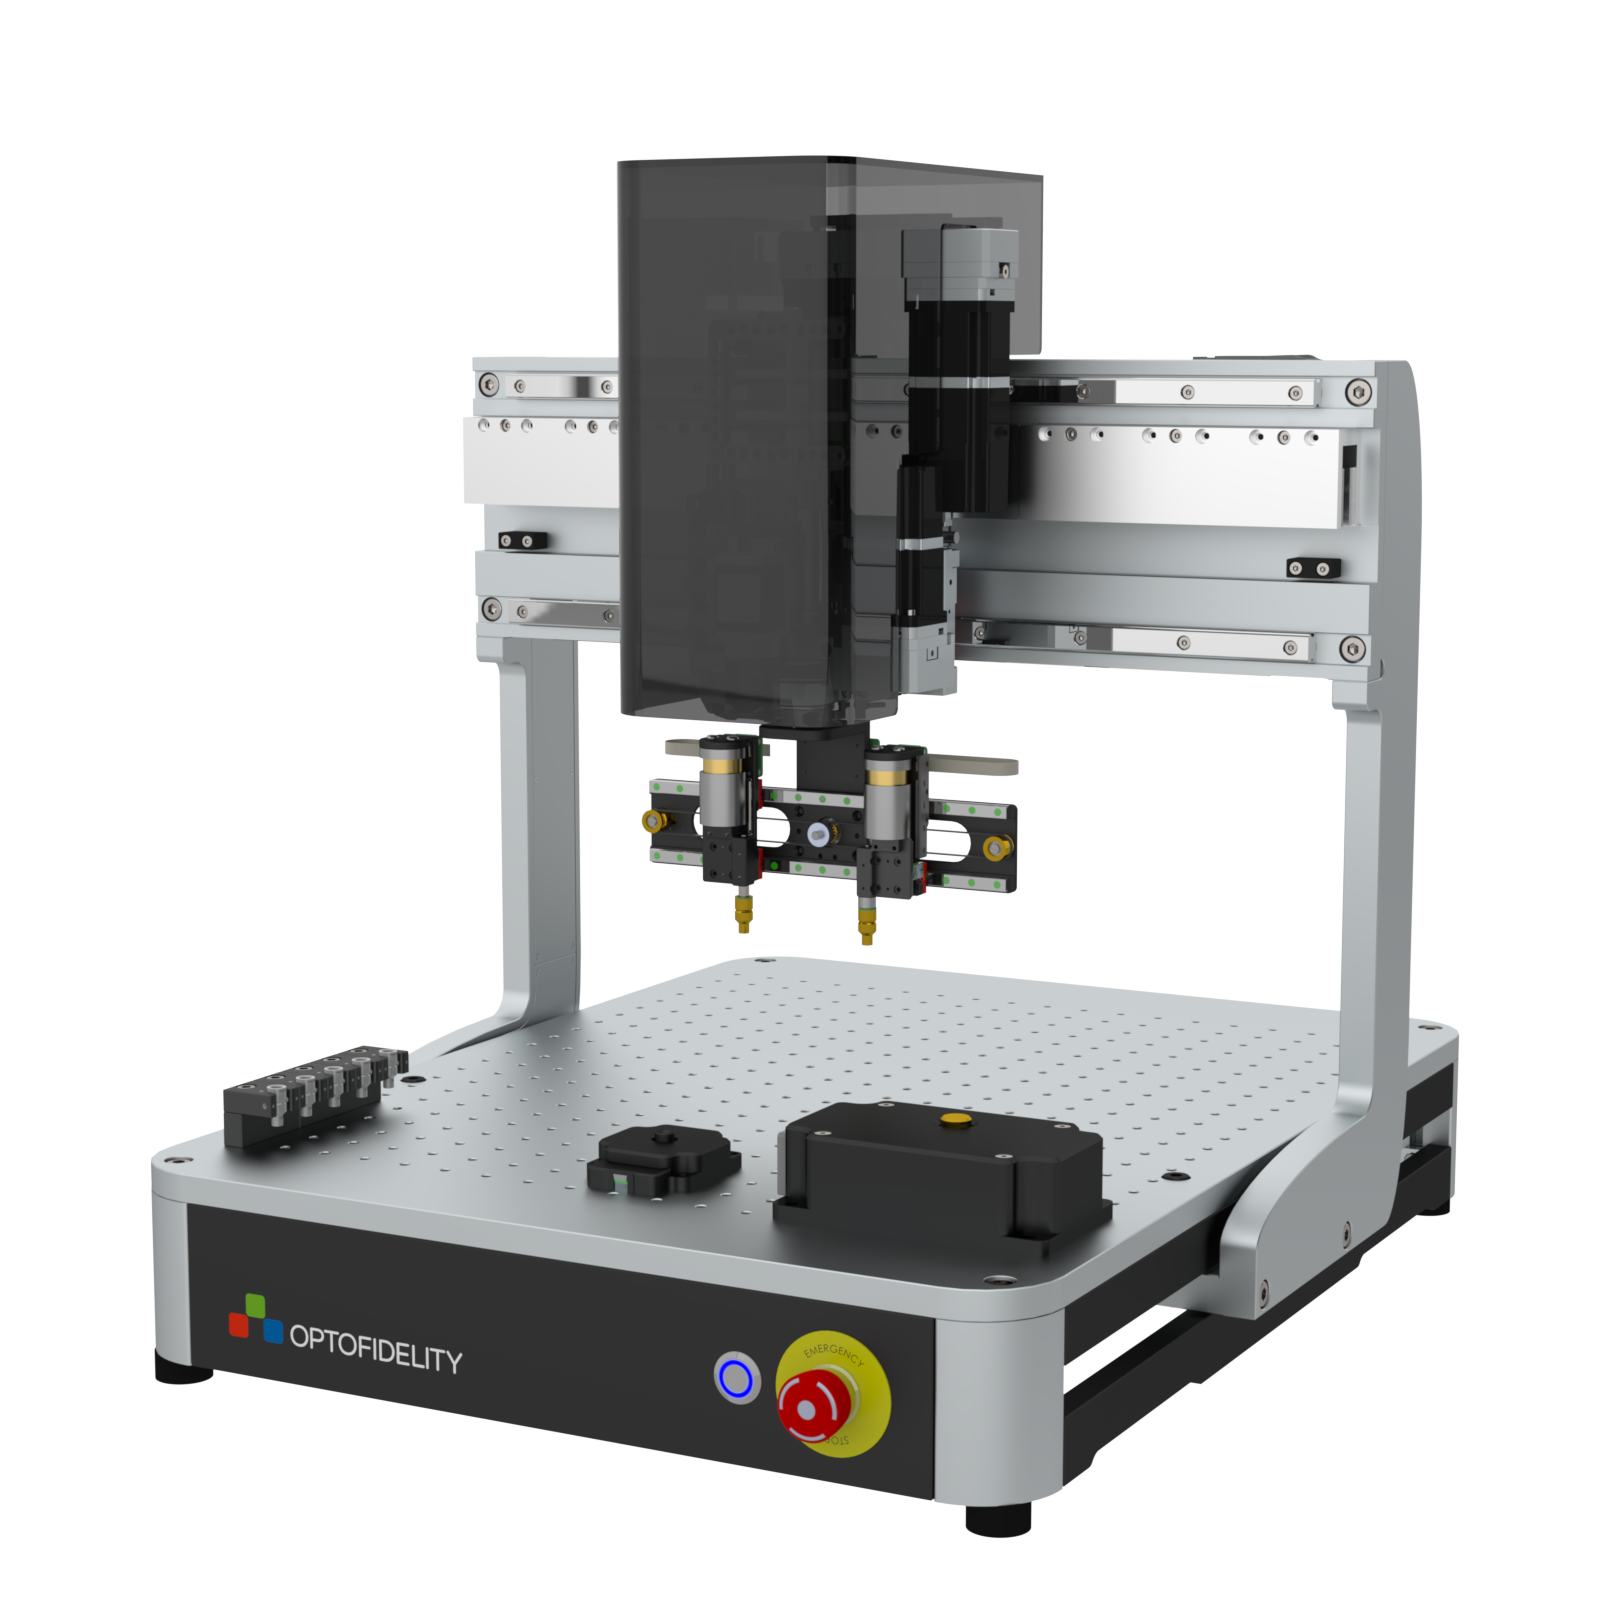
\includegraphics[width=8cm]{synchro_robot.png}
	\caption{Robot with Synchro finger tool. In the workspace from left to right are finger tip rack, Audit gauge for finger and camera offset calibration and Force calibration unit.}
	\label{fig:synchro_robot}
\end{figure}

\section{Software overview}

The core part of the software is TnT (Touch and Test) Server. It is a native stand-alone application that is distributed for Windows and Macos operating systems and installed on a dedicated delivery PC. The PC is further connected to a robot axis controller and other devices such as cameras, calibration tools and so on. The axis controller is typically OptoFidelity proprietary Optomotion controller but also other controllers may be used depending on robot type. Optomotion controls the individual axes of the robot and can be further used for controlling IO channels and trigger signals if necessary for the delivered system. These relations are shown in Figure \ref{fig:server_sw}.

\begin{figure}[!h]
	\centering
	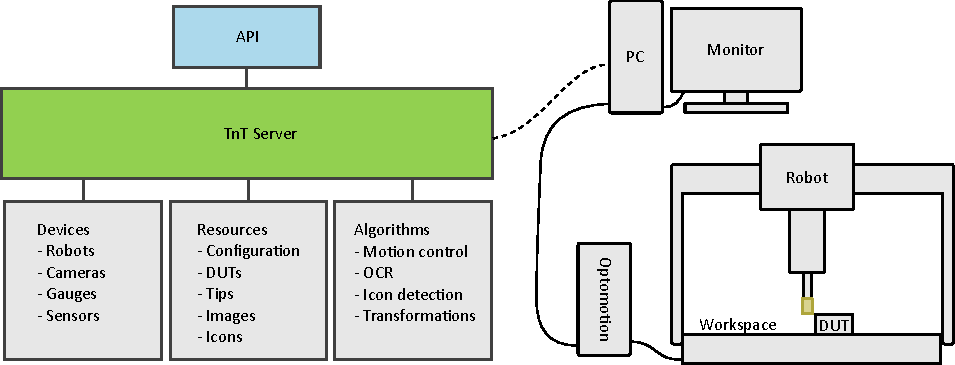
\includegraphics{server_sw.pdf}
	\caption{Illustration of TnT Server, control PC, Optomotion and robot.}
	\label{fig:server_sw}
\end{figure}

On a more detailed level, TnT Server implements drivers for controlling various devices such as robots, cameras, detectors and sensors. It also stores various resources that can be created at runtime and stored to disk for future use. These resources include system configuration, DUT positioning data, tip dimensions, images (from cameras or other sources) and icon shape models. TnT Server also implements algorithms that use the devices and resources. These include robot motion planning and motion control, optical character recognition (OCR), icon detection and transformations between different coordinate systems. These transformation are essential part of the entire system as the resources and devices (e.g. robots and DUTs) usually have specific position and orientation in the 3D space and need to be treated in relation to each other. The DUT coordinate system is very useful in most typical use cases. For example, when user wants to write scripts where gestures are performed on DUT, the DUT needs to be positioned in the workspace only once and then the local DUT coordinates can be used in scripting to keep things simple.

TnT Server, as the name implies, is actually an HTTP server. Once it has successfully initialized, it will just wait for incoming requests via REST API. These requests can for example move the robot to given position, return current robot position, create new DUTs, find an icon from existing DUT using a camera, just to name a few.

\begin{figure}[!h]
	\centering
	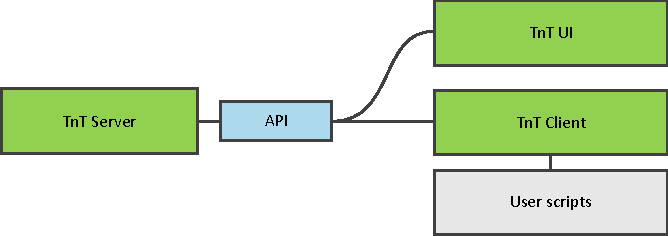
\includegraphics{server_client.pdf}
	\caption{TnT Server and other software components communicate via REST API.}
	\label{fig:server_client}
\end{figure}

TnT Server is capable of controlling the entire system, but usually it is not very accessible as such. Users are provided with more productive ways of using the API. The most basic way is by use of TnT Client. This is a client side implementation of the API in some specific programming language, most typically Python. It documents what the API can do and what parameters can be provided. Users can create virtually any type of test scripts based on TnT Client. It is also advised to use TnT Client instead of the REST API directly as OptoFidelity aims to keep breaking changes in TnT Client minimal in future versions.

The use of Python TnT Client is very easy. It is a Python package with minimal dependencies and can be ran on the delivery PC or remote PC in normal Python interpreter. Example below shows how to move robot effector 50 mm along the workspace  x-axis:

\begin{lstlisting}[language=Python]
from tntclient.tnt_client import TnTClient

# Create client object. By default connects to localhost.
client = TnTClient()

# Create client object to control the default robot configured in TnT Server.
robot = client.robot("Robot1")

# Move robot from current position 50 mm along the workspace x-axis.
robot.move_relative(x=50)
\end{lstlisting}

More examples and the client API reference can be found inside the provided TnT Client Python package.

For performing the most typical tasks such as positioning DUTs, adding tips and teaching icons, there is TnT UI. It is also a stand-alone application that is typically run on the delivery PC and it interfaces with TnT Server via the API. In principle the UI could be run on a remote PC that is connected to the delivery PC via a network. The interface between TnT Server and other software components is shown in Figure \ref{fig:server_client}. See \autoref{ch:ui} for more detailed description of TnT UI features.

\chapter{TnT Server}
TnT Server is the core of OptoFidelity TOUCH robot systems. It provides functionalities for touch and test applications such as controlling robot and taking camera images. The component is called server because to achieve this functionality it acts as a HTTP server.

\section{Installing/re-installing the Server}
\label{sec:server_installation}

When installing an update to TnT Server, or re-installation is needed, OptoFidelity Technical Support can perform the operation assuming TeamViewer access to the PC is available. See the "Support" section \ref{part:support} for details how to request support.

If you have an installer package available, and want to perform the installation independently, please follow these instruction carefully.

Installation can be done by running the installation package. To run the server a dedicated HASP USB encryption dongle has to be connected to the measurement PC.

\subsection{Windows}

A valid license text file has to be available with the following path: "\tntLicensePath".

The installer is a self-contained exe file which launches a wizard that will help the user through the installation process.

In case the user wants to re-install the Server, the following procedure should be followed in order to keep the configuration unchanged:
%
\begin{enumerate}
	\item \label{itm:server_first} Go to the folder "\tntRootPath" and create a back-up of existing "\tntServerFolder" folder by renaming the folder as "TnT Server 2020-01-02" where the date is the backup date.
	\item Run installation package as usual (the installer will create a new "\tntServerFolder" folder).
	\item Copy "configuration" folder from backup to the new installation.
	\item Under "configuration" folder there should be "client\_config.yaml". If any new features were added to the API, they should be exposed in the client by adding them to correct include lists in this config file. This step can usually only be performed by OptoFidelity personnel.
	\item Generate TnT Client that matches the new server installation. Instructions for this can be found under "\tntServerFolder/client/README.md".
	\item Copy "data" folder from backup to the new installation.
	\item When TnT Server is updated, also TnT UI must be updated to latest version. See Section \ref{sec:ui_installation} for instructions.
\end{enumerate}

After SW has been updated, carefully step through the pre-run checklist in Section \ref{sec:pre_run_checklist}.

\subsection{Macos}

A valid license text file has to be available with the following path: "\tntLicensePathMacos".

The installer is a shell script with embedded data and can be ran from command-line. Once executed, the installer will prompt user to continue installing the package.

In case the user wants to re-install the Server, the following procedure should be followed in order to keep the configuration unchanged:
%
\begin{enumerate}
	\item Run the installation script from any location. The installer will create a backup of existing installation and copy new files under "\tntRootPathMacos\tntServerFolder". 
	\item The configuration and data directories are automatically copied from the latest backup to the new location by the installer.
	\item TnT Client is automatically generated and installed to the global python environment by the installer.
	\item Under "configuration" folder there should be "client\_config.yaml". If any new features were added to the API, they should be exposed in the client by adding them to correct include lists in this config file. This step can usually only be performed by OptoFidelity personnel.
	\item If any changes to "client\_config.yaml" were made, manually generate TnT Client that matches the new server installation. Instructions for this can be found under "\tntServerFolder/client/README.md".
	\item When TnT Server is updated, also TnT UI must be updated to latest version. See Section \ref{sec:ui_installation} for instructions.
\end{enumerate}

After SW has been updated, carefully step through the pre-run checklist in Section \ref{sec:pre_run_checklist}.

\subsection{Pre-run checklist}
\label{sec:pre_run_checklist}

Depending on the content of the update, it is possible, that there are changes affecting some of the previously configured properties, for example positioning of the DUTs, or the lengths of the tools. Therefore it is not recommended to perform any updates entirely remotely. Instead, after software has been updated, the operator should be physically close to the robot to be able to use the emergency stop in case something has changed unexpectedly. Perform the following actions monitoring the robot carefully:
%
\begin{enumerate}
    \item Make sure that the tip attach status of the robot matches the status in the Tips view in the UI i.e. if a tip is attached to robot finger, it should be shown as such in the UI.
    \item Check that all the tips (including multifinger) are properly attached to their racks (in the back of their slots).
	\item Set low robot speed such as 20 mm/s from TnT UI and for each existing DUT, tap the four corners using the "Test Tap" button under DUT view in the UI.
	\item Pick and drop each positioned tip using the controls under Tips view in the UI to make sure that the slot positions are valid.
	\item In case of TPPT delivery: Run worst case lines in Swipe test and run Tap test with sparse grid e.g. 50 mm spacing. Please check that the data is received from DUT and that the gestures function correctly.
	\item In case of HSUF delivery, run a script where icon and text is detected on a DUT and the detected position is tapped.
\end{enumerate}

\section{Starting and closing the server}
\label{sec:server_start}
The server is ran by double clicking the server icon on the desktop. It is also possible to run the "\tntServerExecutable" directly. It can be found from the folder "\tntRootPath\tntServerFolder". The server should open a new terminal window (unless started directly from terminal when the program is run in the existing window). The terminal window shows the server log messages. After the software has started the user can see the following log message in the terminal window "Server ready at port 8000". Additionally, there should be no errors in the log messages. Errors are shown in red and as such they are easily visible when scrolling the terminal window. After server has been started successfully, the configuration that was used will be saved as a backup if there are differences when compared to previous backup. If everything has worked successfully you should see something like in Figure \ref{sec:server_start}.

\begin{figure}[h]
	\centering
	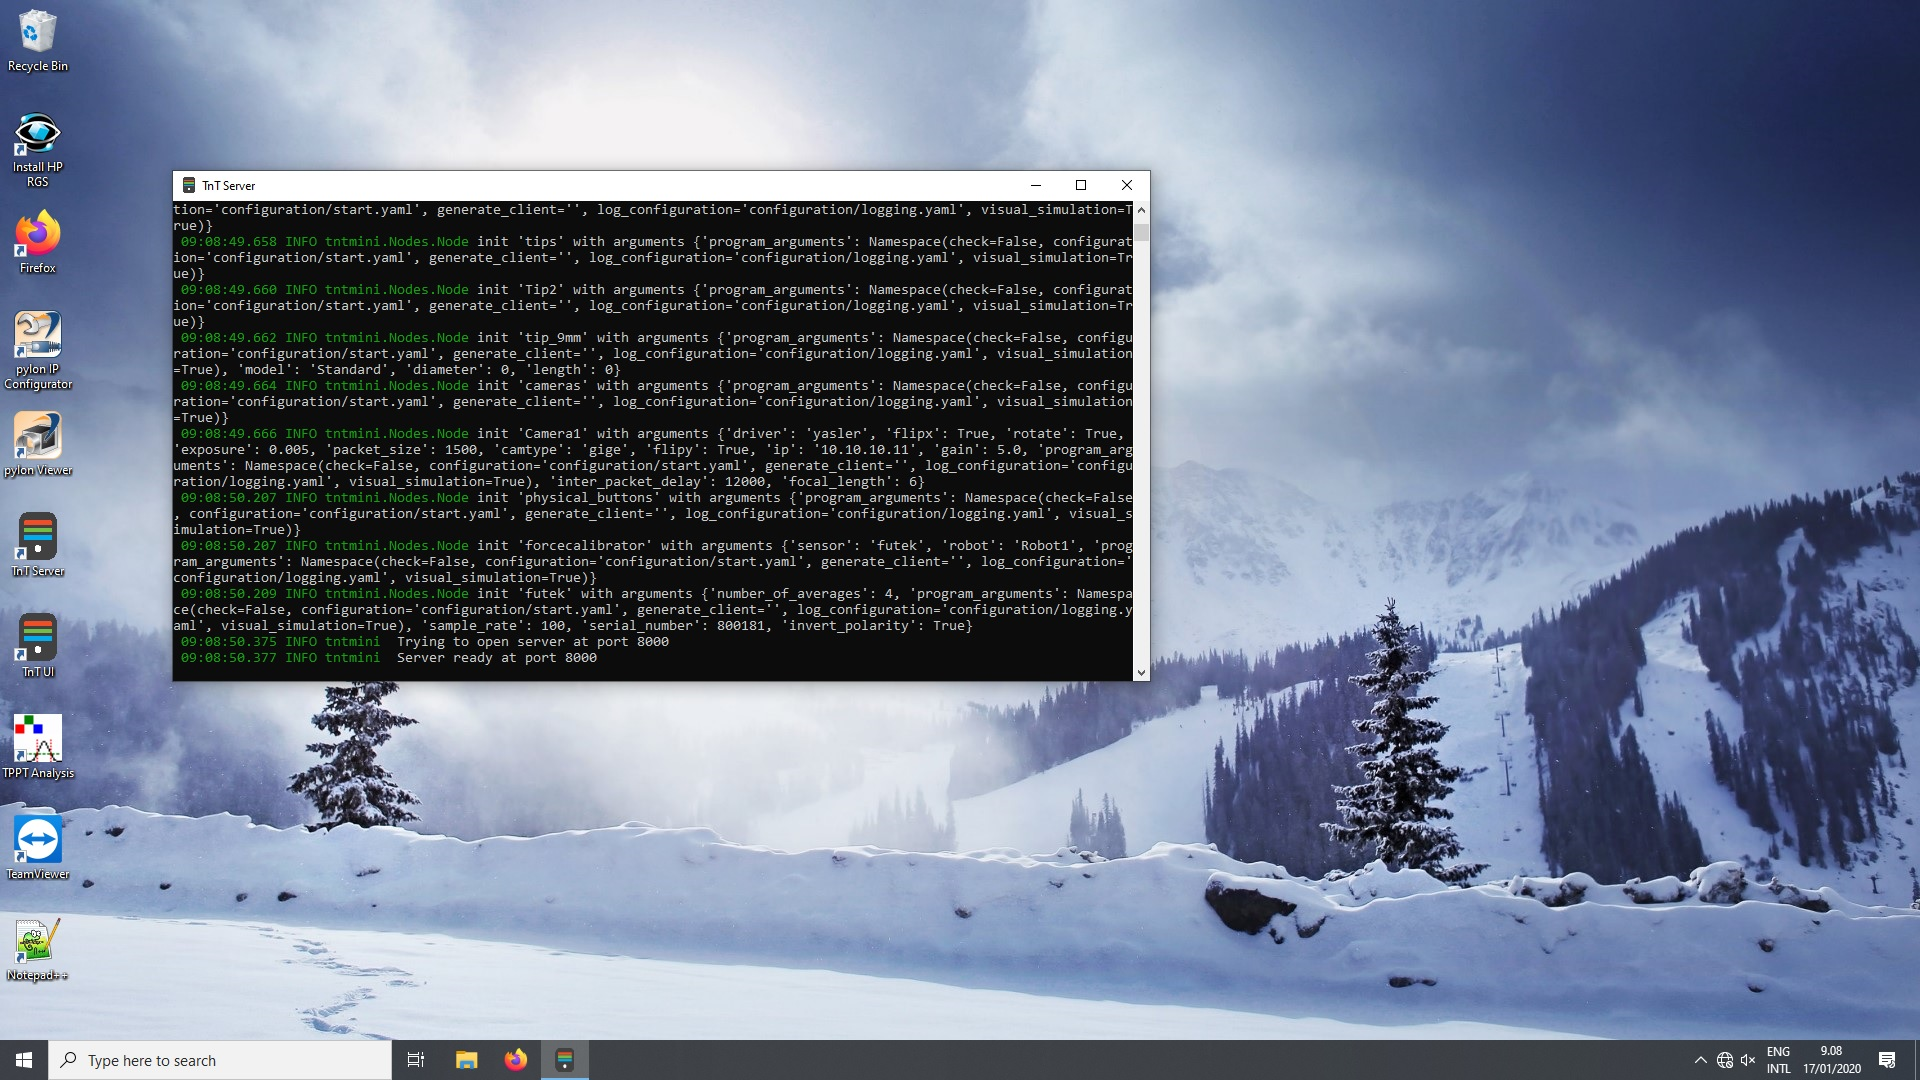
\includegraphics[width=0.7\linewidth]{server_start.jpg}
	\caption{PC after successful server initialization.}
	\label{fig:server_start}
\end{figure}

During a successful start sequence, the robot should home all the axes. This is done every time even though the robot might already be in the home position.

\subsection{Command-line arguments}

Following command-line arguments can be passed to \tntServerExecutable :

\begin{tabular}{ll}
 \texttt{--configuration=[path]} & Path to configuration file. \\
 & Default values is \texttt{"configuration/start.yaml"}. \\ 
\texttt{--configuration-ip=[ip]} & IP address of FTP server where configuration file can be obtained. \\ 
 & Default value is \texttt{"192.168.127.254".}\\
 \texttt{--fetch-configuration} & Fetch configuration file via FTP and save locally as file specified \\
  & by \texttt{--configuration}. Default value is \texttt{false}.\\
 \texttt{--push-configuration} & Push file specified by \texttt{--configuration} to FTP server. \\
  & Default value is \texttt{false}.\\
  \texttt{--log-configuration=[path]} & Path to logging configuration file. \\
  & Default value is \texttt{"configuration/logging.yaml"}.\\
  \texttt{--visual-simulation} & Use visual simulation if simulator is configured?\\
  & Default value is \texttt{true}.\\
  \texttt{--generate-client=[path]} & Generate TnT Client using provided path to client config file.\\
  & Not used by default.
\end{tabular} 

\section{Motion control and safety}

TnT Server is able to plan robot motion in 3D space for multi-axis robots. The robot axes are run synchronously to execute a planned trajectory. User can set the linear speed and acceleration of the robot effector that is used in the motion planning. Due to safety regulations, the software clamps the given speed to \textbf{250 mm/s}. Using speed higher than that requires special safety equipment which is not part of standard delivery. The acceleration specified by user is not limited by software but the individual robot axes have some limited acceleration which limit the effector acceleration.

\warningbox{Using high acceleration such as over 600 mm/s$^2$ requires a heavy-duty table for the robot to avoid wobbling followed by decreased system accuracy.}

The maximum speed and acceleration of individual axes of the robot are limited by several factors such as maximum current draw and voltage and varies between robots. After the trajectory has been planned with given effector speed and acceleration, the resulting axis speeds and accelerations are evaluated. If the maximum speed or acceleration of axes are violated, the duration of the trajectory is scaled so that then motion can be executed within axis capabilities. In this case a warning message is printed to TnT Server log and the motion is executed using smaller speed and acceleration that what user specified.

With synchro finger robot the rotation of azimuth axis while keeping effector stationary often involves x and y axis motion with very high acceleration even if the rotation is fairly slow. Hence, it is common that when azimuth rotation is involved, the software needs to slow down the motion from what user specified.

\warningbox{Even though the effector speed is clamped to 250 mm/s, the axes can move faster during motion if rotary axes are involved in synchronous motion with prismatic axes. Often the y-axis carries a lot of weight so user must be aware.}

\section{Simulator}

TnT Server can be run as simulator in the absence of physical robot. The simulator can be run in visual mode where the robot 3D model is used to visualize the motion or it can be run in non-visual mode where server just simulates the motion numerically and no visual feedback is given.

\warningbox{Simulator is currently intended mostly for development use so the usability is limited and setup is somewhat tricky.}

\subsection{Setting up simulator}

To run simulator with visualization, copy the directory containing required model STL files under

\texttt{\tntServerFolder/tntserver/web/model/}

For synchro robot, there should be a directory named \texttt{synchro\_asvcf}. The model files are not part of normal TnT Server build. They are provided separately if this has been approved as part of the delivery.

To start the server in simulation mode, the \texttt{start.yaml} configuration file under \texttt{\tntServerFolder/configuration/} must have following text at the beginning of the file:

\begin{lstlisting}
- name: tnt
  cls: TnT.TnT
  parent:
  connection:
  
- name: fileserver
  cls: NodeFileServer
  parent: tnt
  arguments:
    path: web
    port: 8010
  connection: tnt

- name: simulator
  cls: NodeSimulator
  parent: tnt
  connection: tnt
\end{lstlisting}

In normal configuration file there only exists the \texttt{tnt} part.

Additionally for node \texttt{Robot1} the value of argument \texttt{simulator} must be set \texttt{true} and value of \texttt{host} must be set to \texttt{127.0.0.1}. For node \texttt{Camera1} the value of argument \texttt{driver} must be set to \texttt{simulator}.

To illustrate only the relevant parts of the configuration file, it should look like following:

\begin{lstlisting}
- name: Robot1
  cls: Synchro.Robot
  parent: robots
  connection: Robot1_base
  arguments:
    host: 127.0.0.1
    port: 4001
    simulator: true
    
- name: Camera1
  cls: TnT.Camera
  parent: cameras
  connection: camera_mount
  arguments:
    driver: simulator
\end{lstlisting}

\subsection{Running numerical simulator}

To run simulator without visualization, TnT Server should be launched with following command:
\begin{lstlisting}
"TnT Server" --visual-simulation=false
\end{lstlisting}

This can be useful for testing that e.g. script execution works without errors without having to wait for the visualization to load.

\subsection{Running visual simulator}

When TnT Server is launched after the configuration changes without additional flags, the visualization should open in browser window and look something like in Figure \ref{fig:simulator}.

\begin{figure}[h]
	\centering
	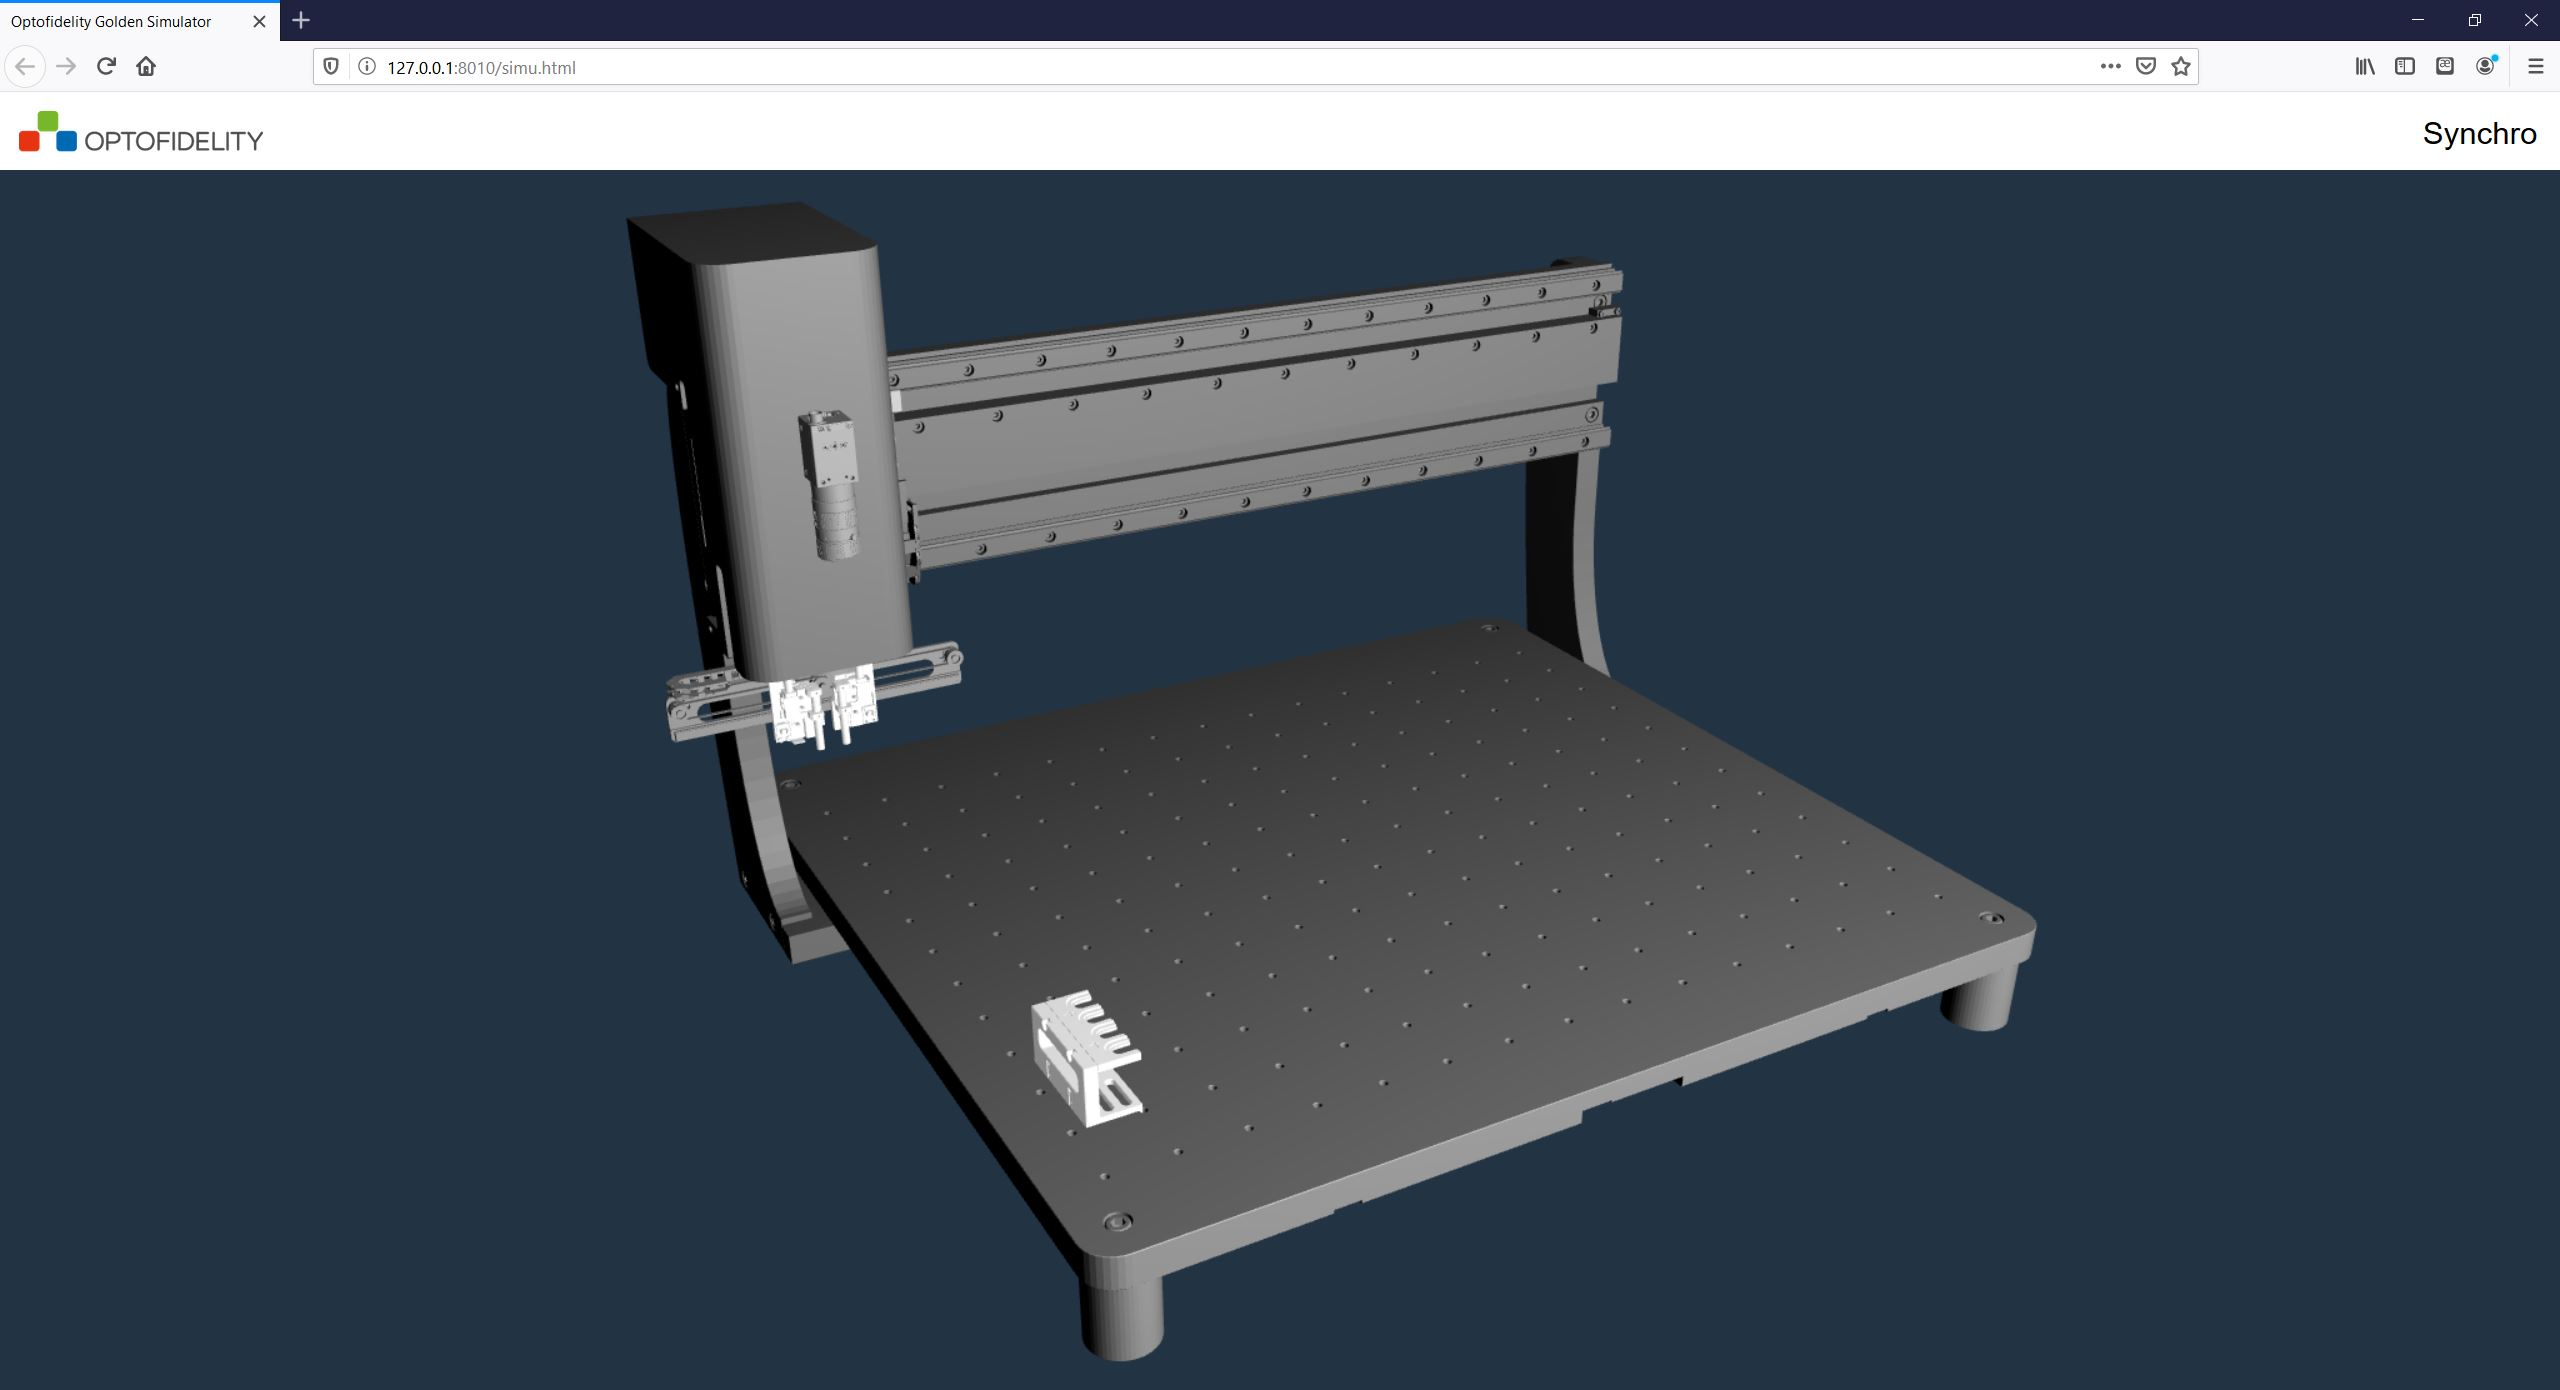
\includegraphics[width=0.7\linewidth]{simulator.jpg}
	\caption{Robot simulator visualization in browser window.}
	\label{fig:simulator}
\end{figure}

\notebox{Sometimes the browser will keep on loading the model for a long time. It may help if you stop the page loading and then refresh it.}

\notebox{The browser window must remain visible in the Windows workspace for the simulation to work. Otherwise motion commands will block forever.}

The view can be controlled by dragging cursor over it. Following controls apply:

\begin{itemize}
\item Left mouse button: rotate view
\item Right mouse button: pan view
\item Mouse wheel: zoom view
\end{itemize}


\subsection{Adding visual content to simulator}

To show a rectangular image object in simulator workspace, add following at the end of the configuration file

\begin{lstlisting}
- name: my_image_object
  cls: NodeSimulatorObject
  parent: ws
  arguments:
    enabled: true
    type: texture
    ppmm: 20
    position: [200, 250, 0, 0, 0, 0]
    image: my_image_file.png
    width: 50
    height: 100
    simulator_parent_object: table
  connection: ws
\end{lstlisting}

The arguments are as follows:

\begin{itemize}
\item \texttt{enabled}: Show object or not.
\item \texttt{type}: Type of simulator object. Value \texttt{texture} is image based texture.
\item \texttt{ppmm}: Pixels per millimeter. Affects the scaling of the object in the simulation workspace.
\item \texttt{position}: List of values \texttt{[pos\_x, pos\_y, pos\_z, euler\_x, euler\_y, euler\_z]}.
\item \texttt{image}: Path to image file relative to server installation directory.
\item \texttt{width}: Width of rectangle in workspace in mm.
\item \texttt{height}: Height of rectangle in workspace in mm.
\item \texttt{simulator\_parent\_object}: Name of parent to which is object is attached to.
\end{itemize}

You can define multiple objects as long as they have different names.

\section{Server troubleshooting}
In this section we have collected the most common issues encountered by our customers. In case you cannot find solution from here, please contact OptoFidelity support. More information about support can be found from Part \ref{part:support}.

\subsection{The terminal window opened during server start is suddenly closed by itself}

To see the error message that appears just before the terminal window shutdown, the user should run the "TnT Server.exe" directly as instructed in Section \ref{sec:server_start}. When the server is run directly in terminal, the window is not closed and the error message remains visible. Usually this type or error is caused by license issues (error related to HASP and bad marshal data). In that case, please make sure that the license file is in the correct place as instructed in Section \ref{sec:server_installation}.

\subsection{Robot does not home itself during start-up}
\label{subsec:robot_not_moving}
This is usually caused by one of the three situations:
\begin{enumerate}
	\item The robot is not powered. To check this make sure that all the cables are plugged in and that the control box switch is in position 1. You should also be able to hear the humming sound of the cooling fan. Additionally when the robot is not powered, you will be seeing error message in server log about attempting to connect an IP address and failing in setting socket properties.
	\item The button next to the emergency stop has not been pushed after the latest start up. If this is the case, the button backlight should be on and you can just press the button. In this case, the log will seem normal at first but when scrolling the terminal window a bit up, you will be able to see error messages about failing robot initialization
	\item Robot is not connected to PC. For this one should check all the Ethernet cables of the installation.
\end{enumerate}

\subsection{Robot fails to reach commanded position}
\label{subsec:robot_positioning_fails}
The robot may be unable to reach a commanded position or the attained position does not exactly match the commanded one. This can happen for a few reasons:
\begin{enumerate}
	\item The position is outside the robot reach, i.e. the movement range limits for one or more joints may be exceeded.
	\item The robot does not have enough degrees of freedom to achieve both the commanded position and orientation. This may occur with e.g. 5-axis robots that have only two rotating joints. Try to position all DUTs parallel to the robot base plate as much as possible to minimize this issue.
\end{enumerate}

\subsection{Issues with camera}
\label{subsec:camera_issues}
These issues are usually found while using the UI. The first thing to check is that the camera is initialized successfully. This can be seen by scrolling up the server terminal window and ensuring that no error messages are there about camera initialization. On the contrary, you should see a log message about successful camera initialization. If there are errors, check that all the Ethernet cables are connected. If there is no initialization message whatsoever, check the configuration file "\tntRootPath\tntServerFolder/configuration/start.yaml" for any camera settings. If none are found, contact OptoFidelity support.


\chapter{TnT UI}
\label{ch:ui}

TnT UI (Touch and Test User Interface) provides a graphical interface for doing following things:

\begin{itemize}
	\item Move the robot
	\item Control camera and view camera image
	\item Calibrate the system
	\item Position tips and DUTs
	\item Position physical buttons
	\item Run Touch Panel Performance Test scripts (if TPPT feature is included)
	\item Create test sequences (if Sequence Generator is included)
	\item Teach icons (if HSUF is included)
	\item Perform User Interface Performance measurements with High speed camera. (if HSUP feature is included)
\end{itemize}

In addition to this user manual, UI also has separate helps embedded in the different views and tooltips in use. The helps can be opened by clicking the white question mark inside a blue circle and tooltip texts appear automatically as tips are hovered on top of the input field. 

\section{Installing/re-installing TnT UI}
\label{sec:ui_installation}
Installation can be done by running the installation package. It launches a wizard that will help the user through the installation process. To run the UI a dedicated HASP USB encryption dongle has to be connected to the measurement PC. 

\subsection{Windows}
A valid license text file has to be available with the following path: "\tntLicensePath".

In case the user wants to re-install the UI, the following procedure should be followed in order to keep the configuration unchanged:
\begin{enumerate}
	\item \label{itm:ui_first} Go to the folder "\tntRootPath"  and create a back-up of existing "\tntUIFolder" folder by renaming the folder as "TnT UI 2020-01-02" where the date is the backup date.
	\item Run installation package as usual (the installer will create a new "\tntUIFolder" folder)
	\item Go to the old folder that you renamed in step \ref{itm:ui_first} and there to the "configuration". In that folder you should have "logging.yaml" and "start.yaml". Copy those and replace the files in respective folder created during installation.
\end{enumerate}

\subsection{Macos}

A valid license text file has to be available with the following path: "\tntLicensePathMacos".

The installer is a shell script with embedded data and can be ran from command-line. Once executed, the installer will prompt user to continue installing the package.
%
\begin{enumerate}
	\item Run the installation script from any location. The installer will create a backup of existing installation and copy new files under "\tntRootPathMacos\tntUIFolder". 
	\item The configuration directory is automatically copied from the latest backup to the new location by the installer.
\end{enumerate}

\section{Starting up}

\begin{figure}[h]
	\centering
	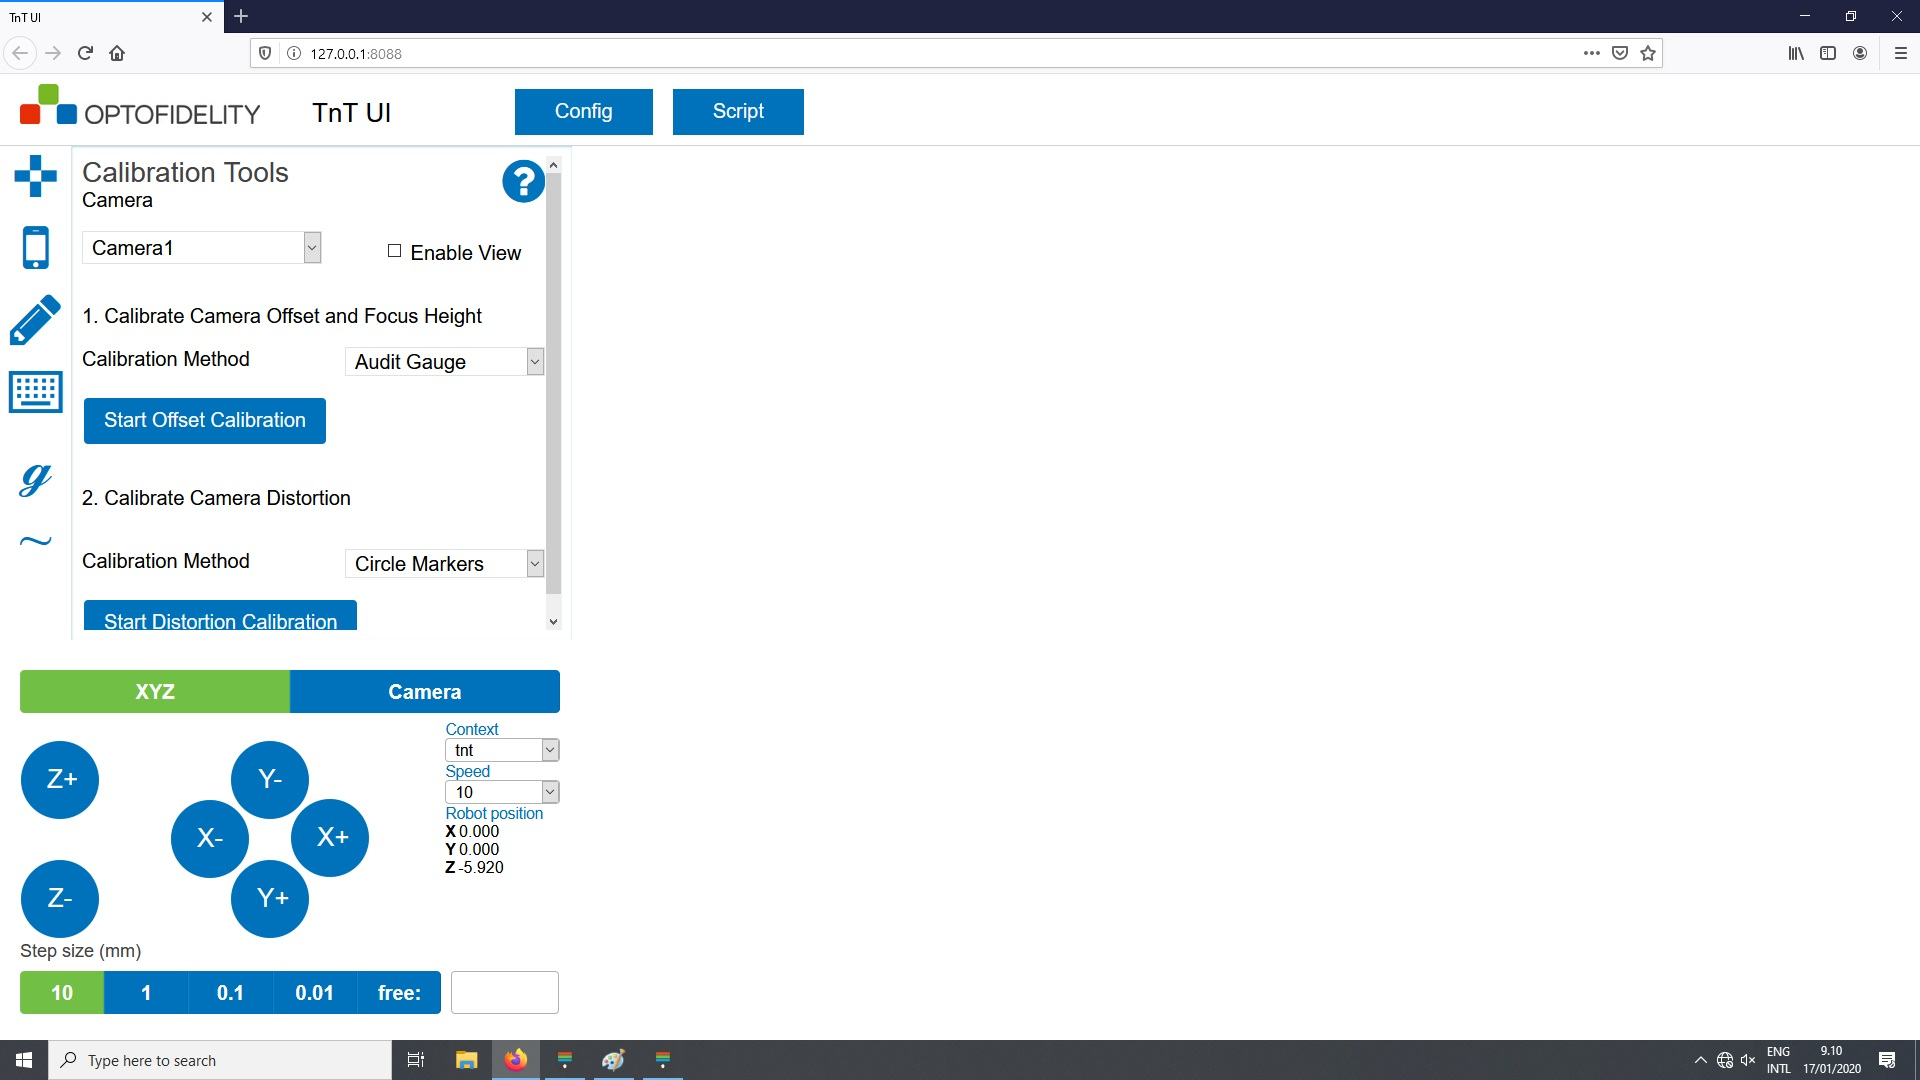
\includegraphics[width=0.7\linewidth]{ui_start.jpg}
	\caption{PC after successful UI initialization.}
	\label{fig:ui_start}
\end{figure}

Before starting UI, please make sure that the server has successfully been started. The UI can be started by double clicking the icon on the desktop. It is also possible to run the "\tntUIExecutable" directly. It can be found from the folder "\tntRootPath\tntUIFolder". It should first initialize a new terminal window and then open web browser (if not yet open) and show UI in address http://127.0.0.1:8088/. Please refer to Figure \ref{fig:ui_start} to see how PC should look like after successful UI initialization.

\section{Camera calibration}

\begin{figure}[h]
	\centering
	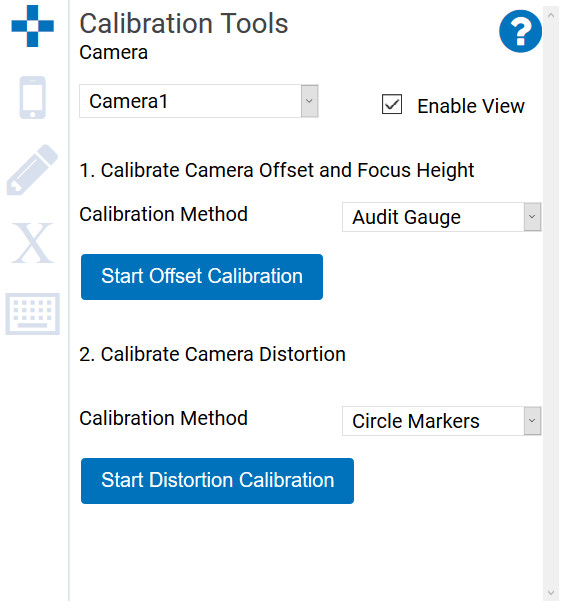
\includegraphics[width=0.4\linewidth]{ui_camera_calib.jpg}
	\caption{Camera calibration view in TnT UI.}
	\label{fig:ui_camera_calib}
\end{figure}

TnT UI Config page has a view for camera calibrations as shown in Figure \ref{fig:ui_camera_calib}. These must be performed before camera can be used in any actual operations such as moving robot from camera image, positioning DUTs using camera or performing functional testing.

Camera calibrations are done during delivery bring up by Optofidelity engineers. User may need to repeat the calibrations in case anything related to camera changes. This could be change in camera focus distance or change of camera objective.

\input{from_ui_repo/camera}


\section{Position DUTs}

This section contains instructions for positioning DUTs with the TnT UI. The UI Configs page has DUTs view for DUT positioning as shown in Figure \ref{fig:ui_duts}.

\begin{figure}[h]
	\centering
	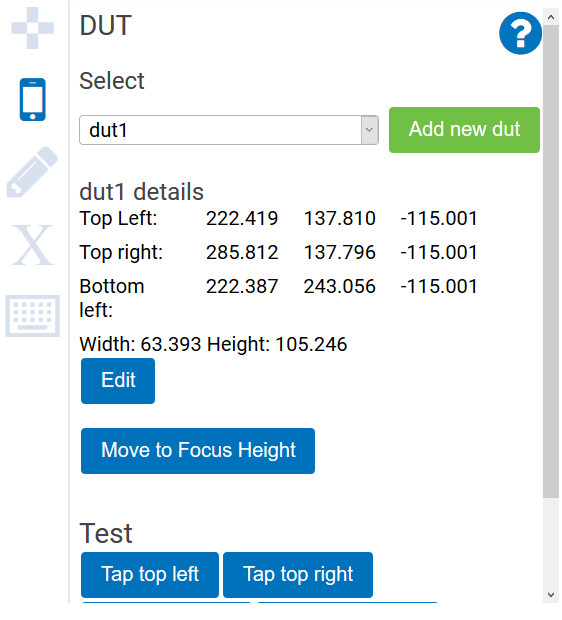
\includegraphics[width=0.4\linewidth]{ui_duts.jpg}
	\caption{DUT positioning view in TnT UI.}
	\label{fig:ui_duts}
\end{figure}

\input{from_ui_repo/duts}
 
\section{SVG shapes for a DUT}
For non rectangular DUTs the TnT software suite offers a possibility to define the shape as an SVG image. The SVG can be created using any suitable software, for example Inkscape. The SVG is added in the DUT edit pane and which stores it in "\svgFilePath".

A rough guide to SVG drawing with Inkscape can be found from Appendix \ref{app:inkscape_guide}.

\subsection{SVG shape requirements}
\label{sec:svg_shape_requirements}
In the SVG file, two regions need to be defined as paths:
\begin{enumerate}
	\item \texttt{analysis\_region}: This is the region to be tested.
	\item \texttt{bounding\_box}: This is the smallest rectangle that contains the whole analysis\_region. 
\end{enumerate}

It is important that both two regions are named exactly as above and that both of them are paths (not, for example, rectangles or circles). Also, both paths need to belong into same group, the name of the group does not matter. The size of the regions must be the same as the DUT size. Please see figure \ref{fig:svg_example} for reference. 

\begin{figure}[h]
	\centering
	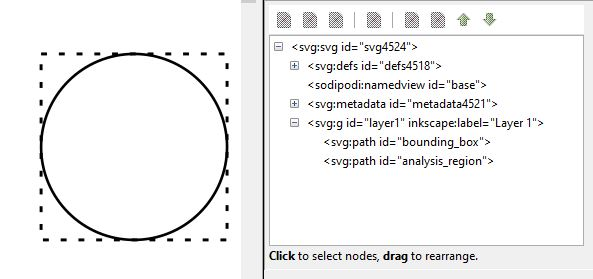
\includegraphics[width=0.7\linewidth]{svg_example.jpg}
	\caption{Example of SVG shape for a round DUT in Inkscape. The solid line shows the analysis\_region and the dashed line the bounding\_box.}
	\label{fig:svg_example}
\end{figure}

\warningbox{If the size of SVG shape does not match with actual DUT size, the TPPT test patterns might be missing lines and points in the edge areas.}

\subsection{The usage of SVG shapes}
The main usage of SVG shapes is to filter lines and points in TPPT scripts so that the robot does not try to touch areas outside the non-rectangular DUTs. Please see Figure \ref{fig:patterns_svg_filtered} for reference.  You can find example SVG (EmulatorRound.svg) from server resources folder in the server installation.

\begin{figure}[h]
	\centering
	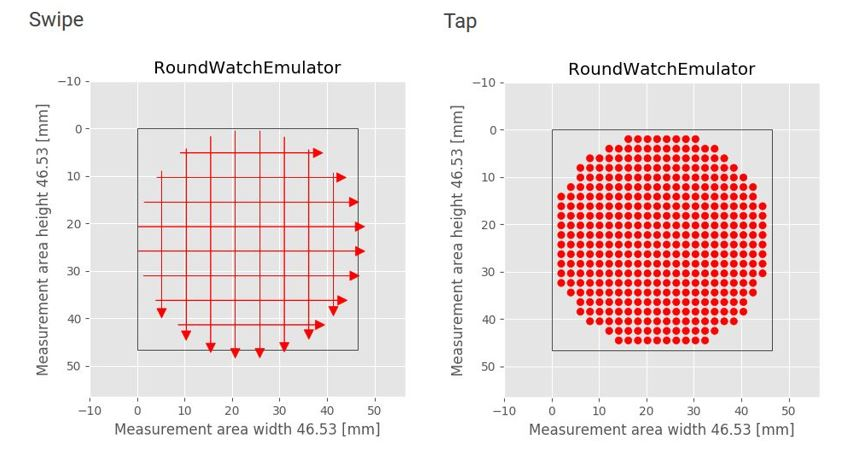
\includegraphics[width=0.7\linewidth]{patterns_svg_filtered.jpg}
	\caption{Examples of swipe and tap test grids for a round DUT}
	\label{fig:patterns_svg_filtered}
\end{figure}

In addition, the positioning image in the automatic DUT positioning is affected by SVG shapes and the image looks different depending on whether the DUT has an SVG shape defined or not. If there is no SVG defined for the DUT, the algorithm uses generic parameters for drawing the positioning image (such as ppmm). If the SVG shape is defined, the algorithm can calculate the exact parameters. However, for most cases, the automatic positioning works similarly with and without an SVG image.

\section{Tips}

\begin{figure}[h]
	\centering
	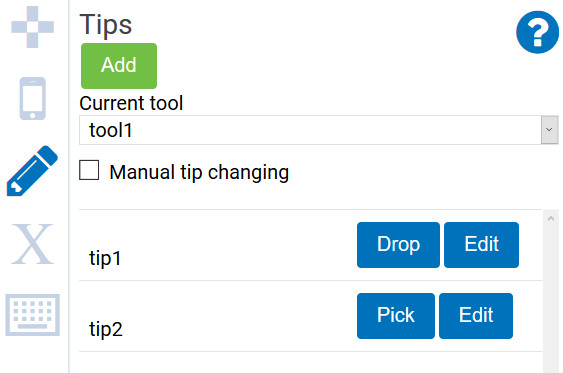
\includegraphics[width=0.4\linewidth]{ui_tips.jpg}
	\caption{Tips view in TnT UI.}
	\label{fig:ui_tips}
\end{figure}

Tip can be added, deleted and attached/detached to robot from TnT UI Config page in Tips view as shown in Figure \ref{fig:ui_tips}.

\input{from_ui_repo/tips}

\section{Icon teaching}
\label{sec:ui_icon_teaching}

\begin{figure}[!h]
	\centering
	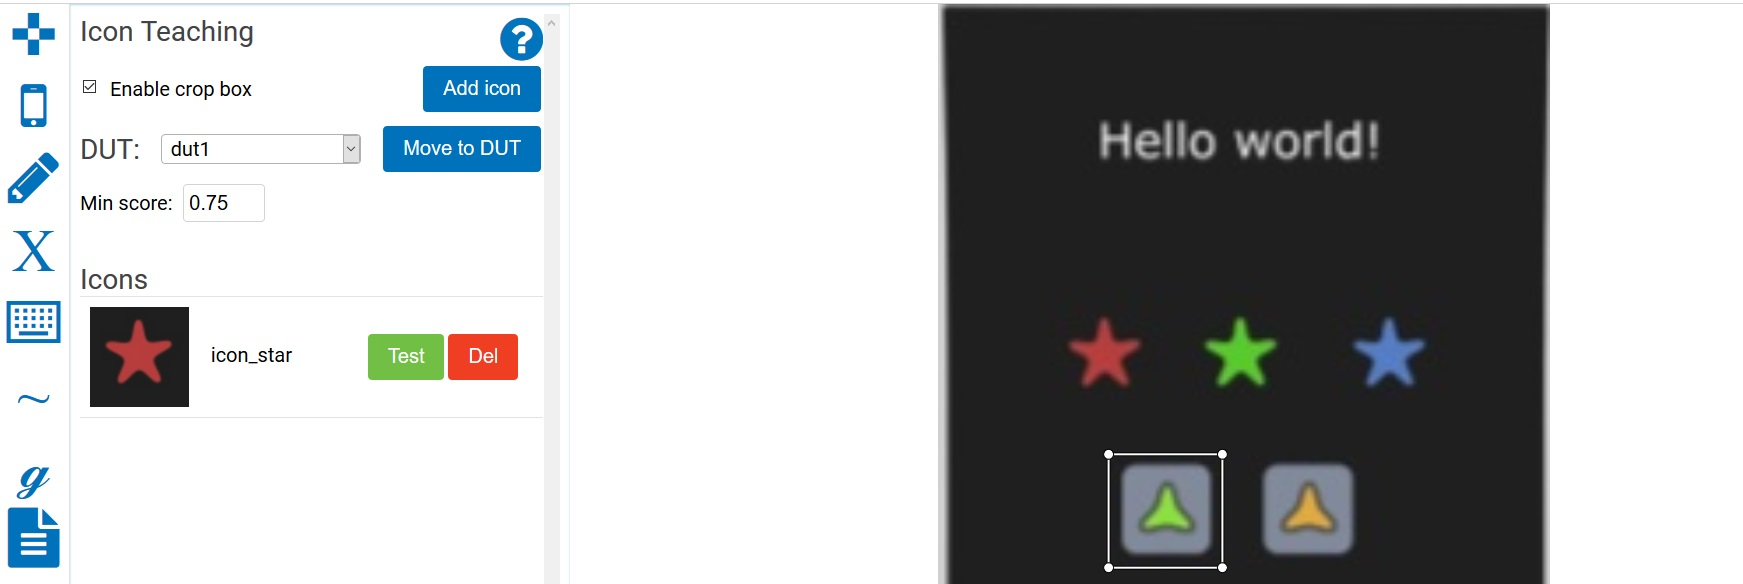
\includegraphics[width=\linewidth]{ui_icon_teaching.jpg}
	\caption{Icon teaching view in TnT UI. On the left side user can create, delete and test icons. On the right user can see the DUT in camera view and adjust crop box to define new icons.}
	\label{fig:ui_icon_teaching}
\end{figure}

TnT UI has "Icon teaching" view under "Config" page where user can teach icon models by using camera view and a crop box. This is shown in Figure \ref{fig:ui_icon_teaching}. The cropped image and icon shape model are stored in TnT Server under \texttt{data/icons} directory so that they can be later used via TnT Client to build functional testing scripts. Icons can also be created from image data in Python scripts using TnT Client.

\input{from_ui_repo/icon_teaching.tex}

\section{Physical buttons}

Physical buttons can be added, deleted and tested in TnT UI config page in Physical buttons view.

\input{from_ui_repo/phys_button}

\section{Force calibration}
\label{sec:force_calibration}

TnT UI Config page has Force calibration view as shown in Figure \ref{fig:ui_force_calib} to calibrate voicecoil based force actuator.

\begin{figure}[h]
	\centering
	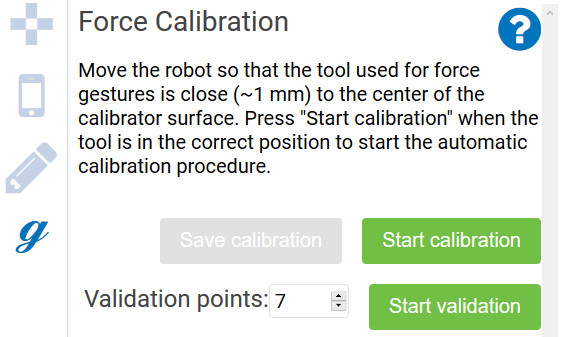
\includegraphics[width=0.4\linewidth]{ui_force_calib.jpg}
	\caption{Force calibration view in TnT UI.}
	\label{fig:ui_force_calib}
\end{figure}

\input{from_ui_repo/force_voice_coil}

\input{from_ui_repo/force_closed_loop}

\section{IO}

TnT UI Config page has IO (Input and Output) view as shown in Figure \ref{fig:ui_io}.

\begin{figure}[h]
	\centering
	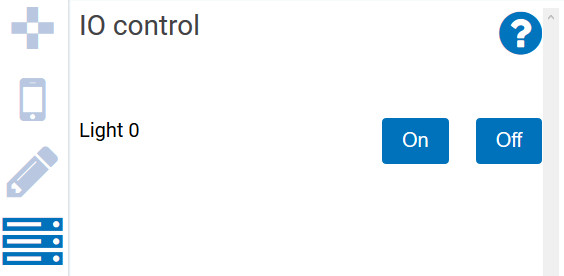
\includegraphics[width=0.4\linewidth]{ui_io.jpg}
	\caption{IO view in TnT UI.}
	\label{fig:ui_io}
\end{figure}

\input{from_ui_repo/io}

\section{Sequence generator}

\input{from_ui_repo/sequence_generator}

\section{UI troubleshooting}
In this section we have collected the most common issues encountered by our customers. In case you cannot find solution from here, please contact OptoFidelity support. More information about support can be found from Part \ref{part:support}.

\subsection{Common notes}
Many of the issues that are found when using UI are originating from server. The following list will provide you with links to the server troubleshooting:
\begin{itemize}
	\item Robot not moving, please refer to Section \ref{subsec:robot_not_moving}
	\item Camera image not shown, please refer to Section \ref{subsec:camera_issues}
\end{itemize}

\subsection{Camera distortion calibration fails}
 This can be caused by various reasons. Ensure that the entire chess pattern target is visible in the camera view. Adjust the exposure and/or gain until the image is clear, sharp, and with good contrast. The chess pattern should be plain black and white, without shades or reflections. It might be necessary to adjust the room lighting or use something to shadow the reflections away.

\subsection{Audit gauge lit inlet is not found automatically}
The reason for this is usually in camera settings or lighting conditions. Try to adjust camera exposure and/or switch off lights in the room.

\subsection{Automatic DUT positioning: cannot find blobs}
The reason for this is usually in camera settings or lighting conditions. Try to adjust camera exposure and/or switch off lights in the room. Also the brightness of the DUT screen might affect. 

\subsection{Automatic DUT positioning: cannot connect to DUT}
Please check the following things and try to go back to another view and then come back. A successful DUT connection is also shown in server terminal log messages (please note that the DUT name in log differs from the one you have given):
\begin{itemize}
	\item Check that the DUT is connected to the correct WiFi network.
	\item Check that the IP address is correct in the DUT app.
	\item Check that the DUT name is the same in the UI and DUT app.
\end{itemize}

\subsection{Adding SVG: The SVG dimensions do not match the DUT dimensions}
First check that the SVG is drawn correctly. If you have used Inkscape for drawing the DUT, please check also that the dimensions are shown as geometrical dimensions and not as visual dimensions. This can be done by going to "Edit"->"Preferences"->"Tools" and making sure that the "Geometric bounding box" is selected.

\chapter{OptoTouch DUT applications}
In order to communicate with phones or tablets, a specific DUT application needs to be used. This chapter discusses different DUT applications and their usage.

\section{OptoTouch Android}
OptoTouch Android implements three different functionalities: pen-to-ink (P2I) testing, watchdog (WD) testing, and touch testing. Additionally, it is needed for accurate DUT positioning with both manual and automatic methods. Currently, the latest version of the app cannot be found from app store but it is delivered as APK (android installation package) with the projects.

\tipbox{If touch testing is going to be done, the app should be opened in \emph{pinned mode} if possible. This prevents accidentally swiping any menus open that might prevent the app to function properly.}

\notebox{Remember that the DUT name must be \emph{exactly} the same in the server and the DUT application.}

\begin{wrapfigure}[20]{r}{0.3\linewidth}
	\centering
	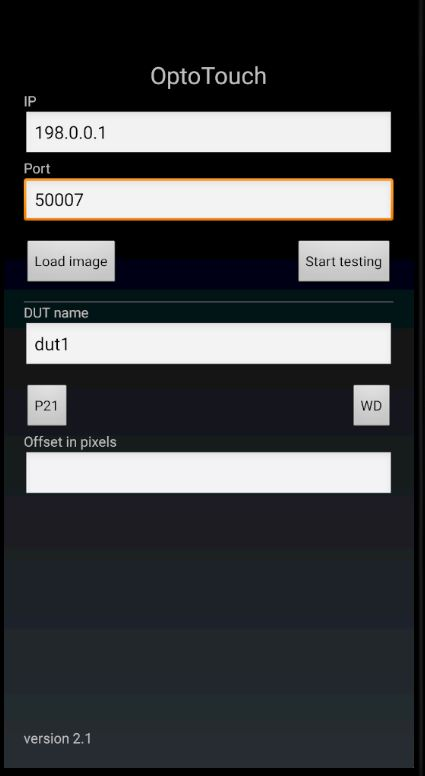
\includegraphics[width=0.8\linewidth]{OptoTouch_Android_main_view.JPG}
	\caption{Main view of OptoTouch Android application.}
	\label{fig:optotouch_android_main}
\end{wrapfigure}

% This text needs to be refined
When app is launched, the main window opens (Fig \ref{fig:optotouch_android_main}). All the functionality can be accessed from the main window. The fields are as follows from top down and right to left:
\begin{itemize}
	\item \texttt{IP:} IP address of the PC the the app is connected. See Subsection \ref{subsec:touch_testing} for more details.
	\item \texttt{Port:} The port to which the app is connected in the PC. See Subsection \ref{subsec:touch_testing} for more details.
	\item \texttt{Load image:} Opens a dialog box for loading an image from DUT memory and shows it on the screen.
	\item \texttt{Start testing:} Connects the DUT to PC for touch testing and automatic positioning. See Subsections \ref{subsec:touch_testing}, \ref{subsec:dut_positioning_features}, and \ref{subsec:communication_with_server} for more details.
	\item \texttt{DUT name:} The name of the DUT given in TnT server. See Subsection \ref{subsec:touch_testing} for more details.
	\item \texttt{P2I:} Opens pen-to-ink measurement view. For more information see \ref{subsec:P2I}
	\item \texttt{WD:} Opens watchdog measurement view. For more information see \ref{subsec:WD}
	\item \texttt{Offset in pixels (deprecated):} Moves the lit corner pixels closer to the screen center in y-axis direction with given amount of pixels. This is a legacy feature for positioning round corner DUTs and not supported in the newer versions of TnT.
\end{itemize}

\subsection{Touch testing}
\label{subsec:touch_testing}
The touch testing view is shown in Figure \ref{fig:touch_testing}. In the upper right corner the device resolution is shown. Below the page header user can see the socket connection statuses. For more information about the socket communication refer to Subsection \ref{subsec:communication_with_server}.

\begin{figure}[h]
	\centering
	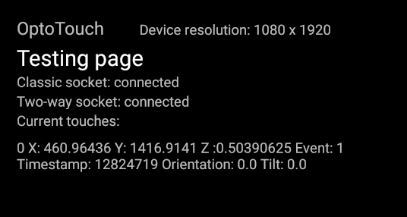
\includegraphics[width=0.7\linewidth]{OptoTouch_Android_touch_testing.jpg}
	\caption{Touch testing view.}
	\label{fig:touch_testing}
\end{figure}

The touch test page also shows the most recent collected touch event data. This information is mainly for debug purposes. The reading showed in the image \ref{fig:touch_testing} tells the following:
\begin{itemize}
	\item \texttt{0:} Touch id given by the operating system to the detected touch. 
	\item \texttt{X:460.96436:} X-coordinate in pixels.
	\item \texttt{Y:1416.9141:} Y-coordinate in pixels.
	\item \texttt{Z:0.50390625:} The pressure number given by the operating system. The exact definition depends on the device and the driver.
	\item \texttt{Event:} The type of touch action that is detected (0 is action down, 1 is action up, and 2 is action move. Basically swipe is something like 0-2-2-2-2-2-2-1)
	\item \texttt{Timestamp:} Androids system uptime in milliseconds.
	\item \texttt{Orientation:} Stylus orientation.
	\item \texttt{Tilt:} Stylus tilt.
\end{itemize}


\subsection{Pen-to-Ink (P2I) testing}
\label{subsec:P2I}
Note that P2I testing requires a HSUP license and special hardware equipment that are not included in a standard delivery.

In the P2I view, the app shows a blank white screen and as the screen is touched, a black line is drawn. When launching this view the user can set the amount of touches that are shown by the black line. The P2I measurement uses high-speed camera to get video image as the robot draws the line and then a machine vision algorithm calculates the latency between finger movement and the end of the drawn line. Refer to Section \ref{sec:HSUP} for more details. 

\subsection{Watchdog (WD) testing}
\label{subsec:WD}
Note that WD testing requires an HSUP license and special hardware equipment that are not included in a standard delivery.

In the WD view, a blank black screen is show and as the screen is touched a white rectangle is shown in the upper right corner of the screen. If the robot finger is equipped with a trigger and a high-speed camera is used, it is possible to measure the touch latency with this view.

\subsection{DUT positioning features}
\label{subsec:dut_positioning_features}
The application supports two modes of positioning:
\begin{enumerate}
	\item \texttt{Manual positioning:} The app main screen has the corner pixels lit with different color than the background. This helps the user focus the positioning camera exactly to the screen corners.
	\item \texttt{Automatic positioning: } Automatic positioning shows a special image on DUT screen that is then recognized with machine vision and used to positioning the DUT. In order to use the automatic positioning, the app has to be in Touch testing mode and two-way socket has to be connected.
\end{enumerate}

\subsection{Communication with server}
\label{subsec:communication_with_server}
The communication between app and server goes through two sockets:
\begin{enumerate}
	\item \texttt{Classic socket:} The app sends constantly all the touch data through this socket and server either collects it or not. On the server side, the classic socket is only opened after TPPT scripts are loaded. On the app side, the classic socket requires the Two-Way socket to be connected. Not having classic socket connection does not prevent the usage of Two-Way socket for e.g. automatic positioning.
	\item \texttt{Two-way socket:} This socket is used for bi-directional communication. Server sends requests and the app replies. This socket is used, for example, to fetch device resolution and send positioning image to the app.
\end{enumerate}


Communication with server is established when the Touch testing mode is entered. The test page shows the statuses of both sockets (see Figure \ref{fig:touch_testing}). The statuses are only updated when the touch testing mode is entered. If the connection is lost it will not reconnect. 

The two parameters (IP address and port) need to be correct in order to have a working connection. The IP address is the one of the measurement PC in the network that connects PC and DUT. The port is basically always 50007 but can be changed. If you need to get the connection through a different port contact OptoFidelity support (more details for that in \ref{part:support})

There are three options to connect the DUT to the server PC:
\begin{enumerate}
	\item \texttt{WiFi:} Connect measurement PC and DUT in the same WiFi network and set the IP address in the app to be the one of the PC in the network. It is also possible to connect the PC directly to the WiFi router with Ethernet cable.
	\item \texttt{USB with tethering:} Connect DUT with USB cable to the measurement PC and enable DUT's network tethering via USB. (DUT does not need to be connected to a network for this.) Then set the IP address in the app to be the one of the PC in the tethered network.  
	\item \texttt{USB with adb (android debug bridge):} Connect DUT to PC via abd and run the following commands.
	\begin{lstlisting}
	> adb reverse tcp:50007 tcp:50007
	> adb reverse tcp:50008 tcp:50008
	\end{lstlisting}
	In the app, set the IP address to be 127.0.0.1.
\end{enumerate}


\section{DUT application troubleshooting}
In this section we have collected the most common issues encountered by our customers. In case you cannot find solution from here contact OptoFidelity support. More information about support can be found from Section \ref{part:support}.

\subsection{Two-way socket not working}
Check that the following things are set correctly:
\begin{itemize}
	\item Check that TnT Server has initialized correctly.
	\item If WiFi connection to PC is used, make sure that PC and DUT are in the same WiFi network or that the PC is connected to the router with Ethernet cable.
	\item Check that the IP address is correct. It is always the PC's address in the network that is used to connect the devices.
	\item Check that the DUT object has been created in TnT Server via e.g. TnT UI and that the DUT name is \emph{exactly} the same in TnT server and DUT app. Also check for accidental whitespace characters.
	\item Check that firewall is not blocking the IP address or port. Try disabling firewall if feasible (the PC should preferably be disconnect from Internet before the disabling). If this fixes the issue, the Firewall settings can then be modified to allow the traffic.
\end{itemize}

\subsection{Classic socket not working}
Check that the Two-way socket is connected and that the TPPT scripts are loaded.

\subsection{App shows that socket is connected but communication is not working}
The socket information is not updated after initialization. Go back in the app by using the DUT's return functionality and tap "Start testing" to get the updated error messages.

\subsection{Connection not working when using USB tethering}
Sometimes when using USB tethering the connection might not work if the ethernet adapter is in DHCP mode. In this case it might help to set a static IP address.
\chapter{Gestures}
Gestures are configurable robot movements, which mimic the human interactions with a touch panel. The available gestures depend on the robot model in use.

Gestures are executed via Python scripts using TnT Client Python package. Each gesture is a function that takes a varying number of parameters and the function execution returns when the motion is complete. See TnT Client reference manual for detailed description of the available parameters.

\warningbox{The software has very little parameter range validation and there is no collision detection in motion planning. Be very careful when performing gestures with given parameters and make sure the DUT is correctly positioned. It is always best to use low robot speed and acceleration when performing gestures for the first time or when changing parameters.}

\begin{figure}[h]
	\centering
	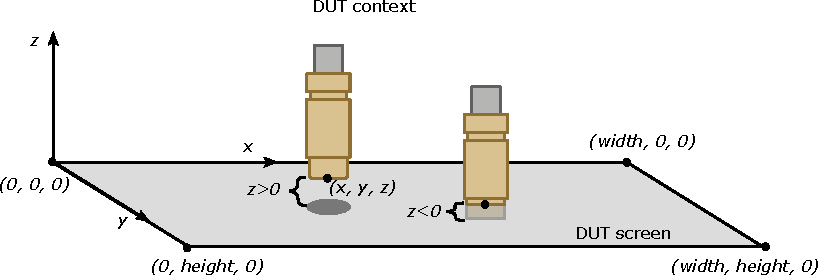
\includegraphics{dut_context.pdf}
	\caption{Illustration of DUT context. The x, y and z direction vectors define the DUT orientation in the embedding workspace.}
	\label{fig:dut_context}
\end{figure}

All gestures have a few common parameters. These are \emph{x}, \emph{y} and \emph{z} coordinates which determine the starting position of the gesture in DUT context. DUT context is a coordinate system where x and y define the "top left" corner of typical display where also the panel reports display coordinate (0, 0). The z-coordinate is zero at the DUT surface and increases upwards from the surface. This is illustrated in Figure \ref{fig:dut_context}. Robot will always first move to the given (x ,y, z) position before the actual gesture is performed. Typically the \emph{z} parameter can be omitted, in which case the DUT's \emph{base distance} is used as the z-coordinate. By default the base distance is 10 mm but it can be changed for each DUT by the user using TnT UI or TnT Client. Robot will move to the starting position using straight path from current position. This may cause collision if there are obstacles along this way. For this reason there is a gesture called \emph{jump} which safely moves robot over a DUT by going first to the maximum height. See section below for more details.

\begin{figure}[h]
	\centering
	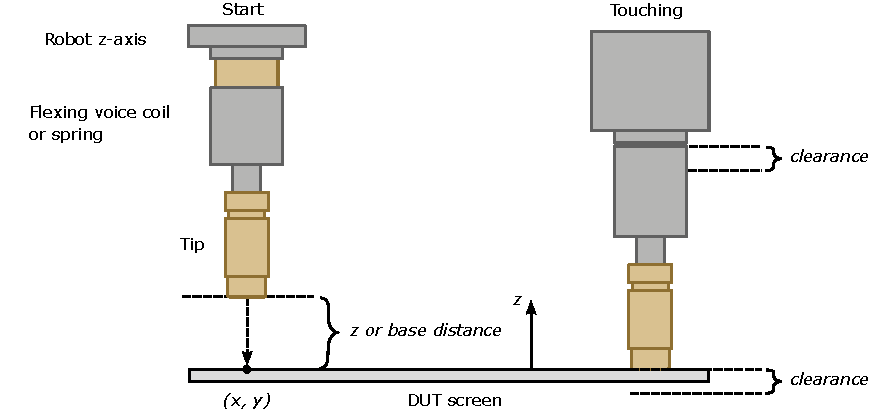
\includegraphics{gesture.pdf}
	\caption{Illustration of typical gesture motion and parameters.}
	\label{fig:gesture}
\end{figure}

Most gestures also have parameter \emph{clearance}, which is the z-coordinate in DUT context when the robot is touching the DUT. Clearance 0 will just barely touch the DUT surface while clearance -1 mm causes robot to press against the DUT when robot tries to move the effector 1 mm below the DUT surface. Most robot effectors have a spring or active voice coil which will flex during such motion. This is illustrated in Figure \ref{fig:gesture}. There is a limited amount of flex in the robot so user must be careful to position the DUT correctly and providing reasonable clearance value. Usually it is not advisable to make clearance more negative than -1 mm.

Most basic gestures also take \emph{azimuth} and \emph{tilt} parameters which are angles in degrees in the DUT context. These determine the orientation of the robot effector when the gesture motion is executed. Some robot models lack rotary joints to actually go to given orientation. In such case the parameter values are omitted by the trajectory planner.

Gesture motion takes into account the length of the tip currently attached to the robot tool head so that the effector touches the DUT surface in the same way with different tips. Usually a tip will make the tool roughly 13 mm longer than without tip. Tips can be changed automatically or manually but it is crucially important that the SW book-keeping of currently attached tip matches with the physical world. If for example user manually adds a tip to the robot but the software still thinks there is no tip attached, there is a risk of collision when gesture motion is performed.

Most parameters that affect gesture motion are given as parameters to gesture functions. However speed and acceleration are robot states which must be set using the robot API.


\section{One-Finger gestures}
This section describes the available gestures if the robot has one or more effectors.

\subsection{Jump}

Jump is used to move the robot effector over designated DUT from current position \emph{safely}. Given that direct route from current position over the DUT may be blocked by obstacles, the safest thing in general is to first go to maximum z-coordinate in the workspace context.

Jump will first move from current position to given \emph{jump\_height} if that position is higher than current position. If not, then current position is used as starting point. If jump heigh is not given, robot will rise to the highest possible position. This is the recommended way. After that, robot will move over the given DUT x, y -coordinates and finally go down to given DUT z-coordinate. Jump gesture is illustrated in Figure \ref{fig:tap_jump}

\notebox{It is always best to first jump over DUT e.g. to DUT coordinates (0, 0, 10) before executing any other gestures. Other gestures will just move from current location to the start of the gesture along straight path which poses risk of collision}.

\begin{figure}[h]
	\centering
	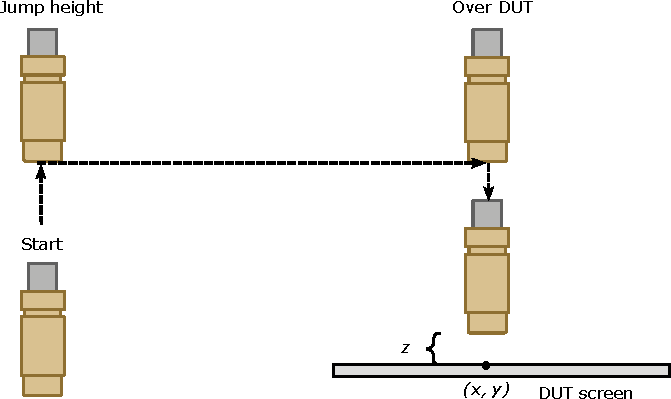
\includegraphics{jump.pdf}
	\caption{Illustration of the jump gesture.}
	\label{fig:tap_jump}
\end{figure}

Jumping over DUT top left corner can be performed with following Python script:

\begin{lstlisting}[language=Python]
from tntclient.tnt_client import TnTClient
client = TnTClient()
dut = client.dut("dut1")
dut.jump(x=0, y=0, z=10)
\end{lstlisting}

\subsection{Tap} 

During a tap gesture the robot first moves over the desired position on DUT at specified z-coordinate or base distance. After that the DUT taps the spot on DUT and returns back to the base distance. The tap duration i.e. how long the tip is in the lowest position can be adjusted. Please refer to Figure \ref{fig:tap_gesture} for illustration.

\begin{figure}[h]
	\centering
	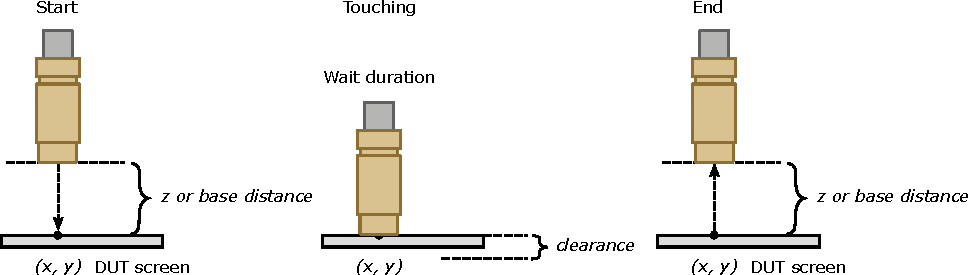
\includegraphics{Tap.pdf}
	\caption{Illustration of the tap gesture.}
	\label{fig:tap_gesture}
\end{figure}

Tap may be performed with the z-axis or by voice coil if robot has such device. Voice coil has a limited movement range so depending on the value of given z-coordinate or DUT base distance, robot may or may not need to first move the z-axis to get to the voice coil operation range. Voice coil has much higher maximum speed and acceleration than the z-axis so if tapping performance is important, user should use z-coordinate or base distance where the robot does not need to use the z-axis when performing consecutive taps.

Tapping DUT top left corner can be performed with following Python script:

\begin{lstlisting}[language=Python]
from tntclient.tnt_client import TnTClient
client = TnTClient()
dut = client.dut("dut1")
dut.tap(x=0, y=0, clearance=-1)
\end{lstlisting}

\subsection{Double tap}

Double tap is similar to tap gesture except that it taps the DUT surface two times. User can specify additional parameter \emph{interval} which is the time the robot waits at lifted position between the two taps. Note that the interval does not take into account the time it takes to move the finger up from the first tap and the time it takes to move the finger down for the second tap. 
Double tap is illustrated in Figure \ref{fig:double_tap_gesture}.

\begin{figure}[h]
	\centering
	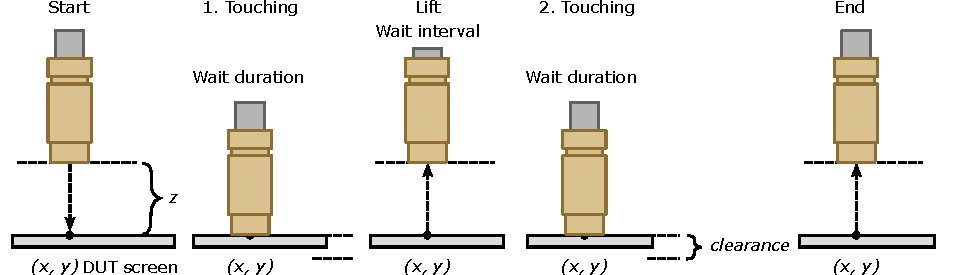
\includegraphics{double_tap.pdf}
	\caption{Illustration of the double tap gesture.}
	\label{fig:double_tap_gesture}
\end{figure}

Double tapping the DUT top left corner with duration 1 s and interval 2 s can be performed with following Python script:

\begin{lstlisting}[language=Python]
from tntclient.tnt_client import TnTClient
client = TnTClient()
dut = client.dut("dut1")
dut.double_tap(x=0, y=0, clearance=-1, duration=1.0, interval=2.0)
\end{lstlisting}

\subsection{Multi tap}

Multi tap is a gesture that performs taps at multiple locations. User provides a list of points where each point is (x, y) position in DUT context where tap is performed. The same could be achieved with multiple calls to the normal tap gesture, but there is certain latency between execution of each tap due to trajectory calculations. If user wants to perform multiples taps consecutively as quickly as possible then multi tap is suitable.

Multi tap also takes parameter \emph{lift} which tells how high effector is lifted between taps.

Multi tapping the DUT at the four corners can be performed with following Python script:

\begin{lstlisting}[language=Python]
from tntclient.tnt_client import TnTClient
client = TnTClient()
dut = client.dut("dut1")
points = [TnTDutPoint(0, 0), TnTDutPoint(dut.width, 0), 
TnTDutPoint(dut.width, dut.height), TnTDutPoint(0, dut.height)]
dut.multi_tap(points=points, lift=2, clearance=-0.5)
\end{lstlisting}

\subsection{Watchdog tap}

Watchdog tap is basically the same as the tap gesture except that it is intended to be used with latency measurements which require a trigger signal from the exact time when the effector touches the DUT surface. There can be different triggering mechanisms but if the robot has voice coil, then the voice coil encoder changes are used as trigger. For this reason, watchdog tap z-motion is always done with the z-axis. Watchdog tap has \emph{trigger\_direction} parameter which can be used to determine whether trigger is signalled from "touch start" or "touch end".

Watchdog tapping the DUT top left corner with trigger signalled from touch start can be  performed with following Python script:

\begin{lstlisting}[language=Python]
from tntclient.tnt_client import TnTClient
client = TnTClient()
dut = client.dut("dut1")
dut.watchdog_tap(x=0, y=0, clearance=-1, trigger_direction="TOUCH_START")
\end{lstlisting}

\subsection{Spin tap}

Spin tap is the same as the tap gesture except that the effector spins around its axis during tap motion. User provides two angle parameter \emph{azimuth1} and \emph{azimuth2} which determine the spin angle when the effector starts to move down and when it reaches the clearance height, respectively. There is also additional boolean parameter \emph{spin\_at\_contact}. If set to true, the rotation happens only after the effector has reached the clearance height.

Spin tap can only be used with robots that have azimuth rotary joint.

Spin tapping the DUT top left corner with rotation of 90 degrees can be  performed with following Python script:

\begin{lstlisting}[language=Python]
from tntclient.tnt_client import TnTClient
client = TnTClient()
dut = client.dut("dut1")
dut.spin_tap(x=0, y=0, azimuth1=0, azimuth2=90, clearance=-1)
\end{lstlisting}

\subsection{Swipe} 
Swipe gesture consists of three separate parts: acceleration, swipe, and deceleration. The acceleration and deceleration are quarter circle arcs of specified radius. The greater the radius the more certain it is that the tip achieves the desired swipe speed (\textit{line drawing speed}) before it touches the DUT screen. Swipe motion is illustrated in Figure \ref{fig:swipe_gesture}a.

\begin{figure}[h]
	\centering
	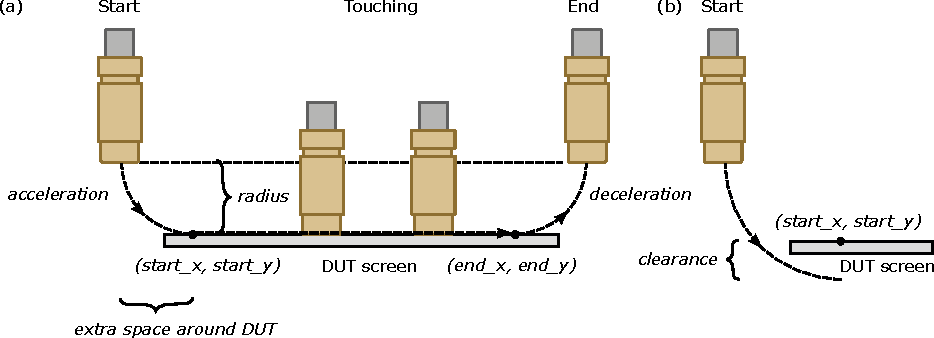
\includegraphics{Swipe.pdf}
	\caption{(a) Illustration of the swipe gesture. (b) Illustration of swipe arc motion when using negative clearance.}
	\label{fig:swipe_gesture}
\end{figure}

\warningbox{Robot may collide with DUT edges during swipe when using negative clearance parameter. Please read this section carefully before using swipe.}

Please note, that due to the arcs the DUT has to be positioned in such a way that the robot can move around it as indicated in Figure \ref{fig:swipe_gesture}a. Occasionally the screen might have high edges and the tip can hit them if the radius is too large. In this case, the user should use zero clearance and use smaller radius. If this does not work then drag gesture might be more appropriate (see Section \ref{sec:drag}). User should notice that the arc is formed towards the start point at the clearance height. Thus if clearance is negative and swipe is started at the very edge of the DUT, there is a risk of collision. This risk is pronounced when using large swipe radius or narrow  tip. This hazard is illustrated in Figure \ref{fig:swipe_gesture}b. It is good practice to start with small clearance such as -0.5 mm and test if it provides sufficient contact with the DUT screen. Sometimes the screens are not perfectly flat which may necessitate the use of more negative clearance values. Then it is best to reduce the swipe radius. Usually 6 mm radius is safe when using tip of diameter 10 mm and clearance -0.5 mm.

The swipe radius gives the robot room to accelerate to target speed so that during touch, the robot speed could be constant. The appropriate radius depends on several factors. Firstly, it may be limited by the collision risk i.e. if swipe starts at the very edge of the DUT and the tip is narrow, user may need to use radius of 6 mm or less. With robot that has voice coil, the arc motion is performed with voice coil which usually has movement range of roughly 9 mm. This also limits swipe arc radius.

The required swipe radius to achieve given speed depends mostly on the acceleration capability of each axis. The slowest axis sets the limit. Usually z axis and voice coil have very high maximum acceleration. Roughly 9000 mm/s$^2$ and 30000 mm/s$^2$ respectively. The x axis can typically reach acceleration of 3000 mm/s$^2$. Typically the y-axis is the slowest, reaching roughly 900 mm/s$^2$. Reaching swipe speed 250 mm/s requires roughly 25 mm swipe radius if acceleration is limited by the y-axis. Due to the difference in the axis accelerations, swipes can be done faster along robot x-axis than along y-axis.

%TODO: Add table and formulas for determining correct radius for different situations.

Swiping across DUT horizontally through the midpoint can be performed with following Python script:

\begin{lstlisting}[language=Python]
from tntclient.tnt_client import TnTClient
client = TnTClient()
dut = client.dut("dut1")
dut.swipe(x1=0, y1=dut.height/2, x2=dut.width, y2=dut.height/2, clearance=0, radius=6)
\end{lstlisting}

\subsection{\label{sec:drag}Drag}
Drag gesture is like swipe but without acceleration and deceleration parts. The tip goes first on top of the line starting point at the base distance. Then it goes directly down, draws the line, stops, and moves back up. With drag the speed might differ a lot during the line movement. However, is some cases with DUT with high/elevated edges or combinations with force measurements, drag is the only feasible option. Please refer to Figure \ref{fig:drag_gesture} for illustration.

\begin{figure}[h]
	\centering
	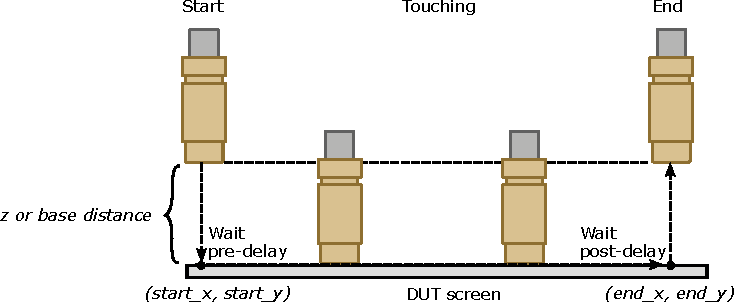
\includegraphics{Drag.pdf}
	\caption{Illustration of the drag gesture.}
	\label{fig:drag_gesture}
\end{figure}

Unlike swipe, drag allows user to specify pre-delay and post-delay to make robot wait until motion along DUT surface starts and until finger lifts off the surface at the end position.

Performing drag across DUT horizontally through the midpoint can be done with following Python script:

\begin{lstlisting}[language=Python]
from tntclient.tnt_client import TnTClient
client = TnTClient()
dut = client.dut("dut1")
dut.drag(x1=0, y1=dut.height/2, x2=dut.width, y2=dut.height/2, clearance=0)
\end{lstlisting}

\subsection{Multiswipe}

% TODO: Gesture should be renamed Multidrag to match other naming.

Multiswipe is the same as the drag gesture except that the robot performs given number of back-and-forth dragging movements on the DUT surface before lifting up. In addition to normal drag parameters, user specifies integer parameter \emph{n} to indicate how many drag movements are performed on the DUT. Value n=1 corresponds to normal drag gesture. Parameter n=2 moves effector from (x1, y1) to (x2, y2) and then back to (x1, y1) and then effector lifts up.

Making a multiswipe across DUT surface can be performed with following Python script:

\begin{lstlisting}[language=Python]
from tntclient.tnt_client import TnTClient
client = TnTClient()
dut = client.dut("dut1")
dut.multiswipe(x1=0, y1=dut.height/2, x2=dut.width, y2=dut.height/2, clearance=0, n=3)
\end{lstlisting}

\subsection{Circle}

In circle gesture the robot moves a circle path on the DUT surface. The given \emph{x}, \emph{y} coordinates define the starting point of the circle which is by default the right edge of the circle. User can specify the radius \emph{r} of the circle and the number of revolutions \emph{n}. The circle is by default done counter-clockwise but user can also set boolean parameter \emph{clockwise} to perform circle in clockwise direction. It is also possible to set parameter \emph{angle} to start the circle at some other point on the circle. The circle gesture is illustrated in Figure \ref{fig:circle_gesture}

\begin{figure}[h]
	\centering
	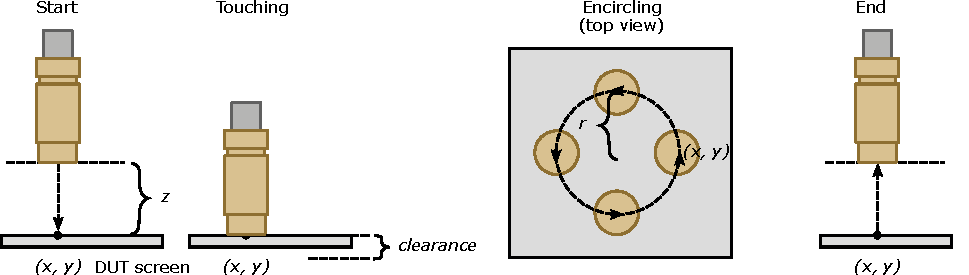
\includegraphics{circle.pdf}
	\caption{Illustration of the circle gesture.}
	\label{fig:circle_gesture}
\end{figure}


Performing circle gesture of radius 30 mm over two revolutions can be done with following Python script:

\begin{lstlisting}[language=Python]
from tntclient.tnt_client import TnTClient
client = TnTClient()
dut = client.dut("dut1")
dut.circle(x=0, y=0, r=30, n=2)
\end{lstlisting}

\subsection{Path}

In path gesture the robot effector moves on DUT through given list of (x, y, z) points along a polyline. Robot will accelerate and decelerate when going from one point to the next so that robot is at full stop at each point. Note that at each point, user can also specify \emph{z} coordinate in the DUT context so that it is possible to lift finger off the DUT surface during path motion. The path gesture is illustrated in Figure \ref{fig:path_gesture}.

\begin{figure}[h]
	\centering
	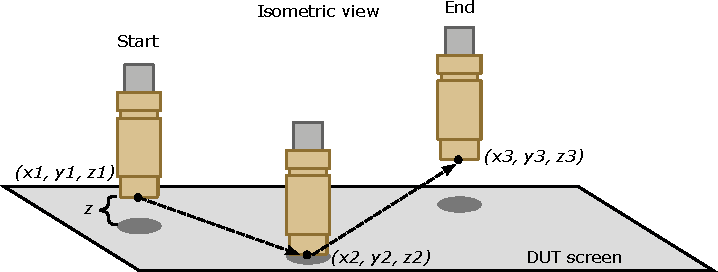
\includegraphics{path.pdf}
	\caption{Illustration of the path gesture.}
	\label{fig:path_gesture}
\end{figure}

Performing path gesture through points (0, 0, 10), (0, 0, 0) and (20, 20, 0) can be done with following Python script:

\begin{lstlisting}[language=Python]
from tntclient.tnt_client import TnTClient
client = TnTClient()
dut = client.dut("dut1")
points = [TnTDutPoint(0, 0, 10), TnTDutPoint(0, 0, 0), TnTDutPoint(20, 20, 0)]
dut.path(points=points)
\end{lstlisting}

\subsection{Smooth path}

Smooth path is the same as the path gesture except that the path connecting the given points is a third-degree spline that interpolates the given points. Unlike path gesture, the effector does not stop at the given points. It will accelerate to the set speed and travel at that constant speed along the spline path and finally decelerate to stop at the final point. The smooth path gesture is illustrated in Figure \ref{fig:smooth_path_gesture}.

\begin{figure}[h]
	\centering
	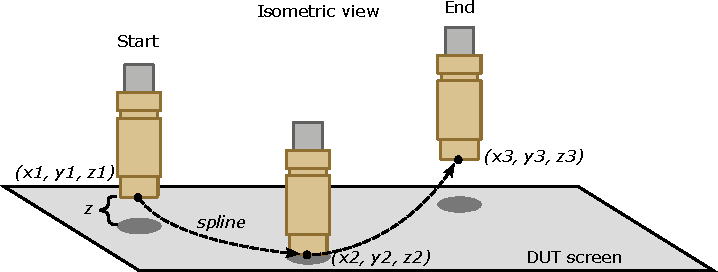
\includegraphics{smooth_path.pdf}
	\caption{Illustration of the smooth path gesture.}
	\label{fig:smooth_path_gesture}
\end{figure}

\warningbox{If the z-coordinates of the points are not the same, the spline path can go to unexpected z-values due to the way spline interpolation works. Path planner tries to detect such unintentional points and raise an error.}

Performing a smooth path gesture through points (0, 0, 0), (20, 0, 0) and (20, 20, 0) can be done with following Python script:

\begin{lstlisting}[language=Python]
from tntclient.tnt_client import TnTClient
client = TnTClient()
dut = client.dut("dut1")
points = [TnTDutPoint(0, 0, 0), TnTDutPoint(20, 0, 0), TnTDutPoint(20, 20, 0)]
dut.smooth_path(points=points)
\end{lstlisting}

\section{Force gestures}

Force gestures are movements on DUT where robot applies given amount of force on the DUT. In standard robots equipped with voice coil the force is generated by moving the effector against DUT with the voice coil until target force is reached. The force is then applied in the direction of the voice coil axis which should typically be close to the normal direction of the DUT plane.

There are two ways to produce force with voice coil: \emph{open loop force control} and \emph{closed loop force control}. Two-finger Synchro robots support only open loop force control. One finger force actuator robots support either open loop or closed loop force control, depending on usage, and selected HW options.

Open loop control is based on the observation that the current draw of the axis is proportional to force. Hence we can construct a look-up table of current-force values by pressing against a reference scale. Then for given target force, the maximum current draw of the axis is set to corresponding value from the table and the effector is pressed against DUT until the current saturates. The look-up table is calibrated once as part of robot setup and then used by gestures later.

% TODO: Here it would be nice to show some plots of curret vs force and also a plot to illustrate the accuracy of open and closed loop force.

Closed loop control is based on active force feedback coupled to the voice coil motion controller. Usually \emph{loadcell} integrated to the axis is used as such feedback device.  Software can then set the axis to move until given force is reached according to the force feedback. The specified force can further be calibrated against a scale to produce a force-force look-up table.

Closed loop force is more accurate than open loop force but it requires dedicated hardware, and is slower to perform due to feedback based active adjustment.

% TODO: Any other characteristics of open loop / closed loop to mention here?

Force calibrations are performed as part of robot delivery using OptoFidelity Force audit and calibration block accessory. User can also perform the calibrations using the Force calibration view in TnT UI in case the calibration becomes invalid for some reason such as change of a hardware part. See Section \ref{sec:force_calibration} for more details.

In the force gesture API force is expressed in \emph{grams of force} denoted gF. It can be converted to Newtons by 1000 gF = 9.80665 N.

\subsection{Press}

Press gesture is similar to tap except that the z motion is planned so that given amount of force is applied on the DUT. User provides parameter \emph{force} to specify how many grams of force is applied on the DUT.

\begin{figure}[h]
	\centering
	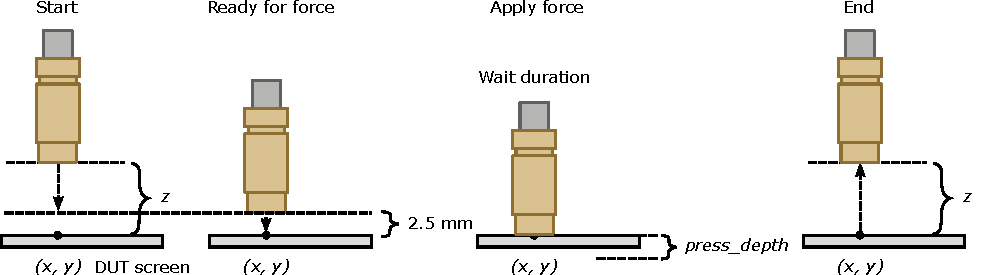
\includegraphics{open_loop_press.pdf}
	\caption{Illustration of the open loop press gesture.}
	\label{fig:open_loop_press_gesture}
\end{figure}

When using open loop force system, user can specify parameter \emph{press\_depth} which is the z-coordinate in DUT context where the effector is attempted to be moved using position control mode. Once the effector hits the DUT surface the voice coil current draw starts to increase until it saturates to the value corresponding to the specified force. The default value of press\_depth is -1 which should normally be sufficient. This parameter has only effect in open loop force mode. Before voice coil is moved, the z-axis is moved so that the effector z-coordinate in DUT context is 2.5 mm. This is to guarantee that the voice coil current saturation works consistently. Open loop press gesture is illustrated in Figure \ref{fig:open_loop_press_gesture}.

\begin{figure}[h]
	\centering
	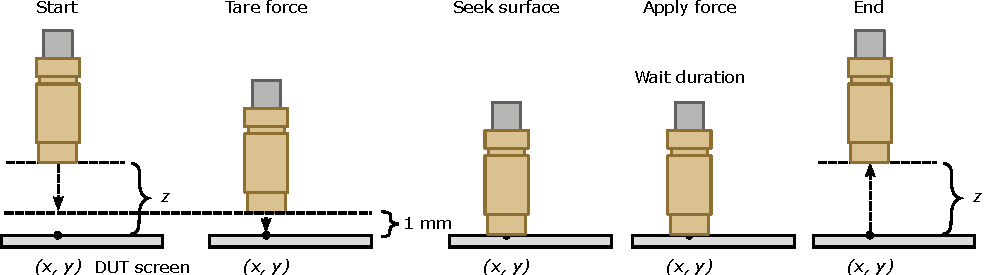
\includegraphics{closed_loop_press.pdf}
	\caption{Illustration of the closed loop press gesture.}
	\label{fig:closed_loop_press}
\end{figure}

When using closed loop force system, the press\_depth parameter is not used because the voice coil firmware is set to force control mode instead of position control. Before force application, the robot performs force tare where the force feedback is zeroed while the effector is not touching the DUT. After tare is complete, the effector is moved to close contact with the DUT surface. Then the voice coil is set to force control mode to apply the given force using closed loop control. The effector must be in contact with the surface when the mode is switched to force control to avoid significant initial overshoot in force. Closed loop press gesture is illustrated in Figure \ref{fig:closed_loop_press}.

Following script can be used to perform press against DUT at DUT xy-origin applying 500 grams of force:

\begin{lstlisting}[language=Python]
from tntclient.tnt_client import TnTClient
client = TnTClient()
dut = client.dut("dut1")
dut.press(x=0, y=0, z=10, force=500, press_depth=-1)
\end{lstlisting}

The API works the same with open and closed loop force except the latter ignores the press\_depth parameter.

\subsection{Drag force}

Drag force is similar to the drag gesture except that a specific force is applied on the DUT while the finger drags over the DUT surface. User provides parameter \emph{force} to specify how many grams of force is applied on the DUT. 

Considering the nature of drag force, there is no guarantee of the applied force being accurate throughout the gesture. During drag, the robot finger is moving along the surface, and for example changes in friction, or inconsistencies in the surface may affect the force momentarily. Generally drag force is more accurate with lower speeds, as the system has more time to adjust to changes.

\begin{figure}[h]
	\centering
	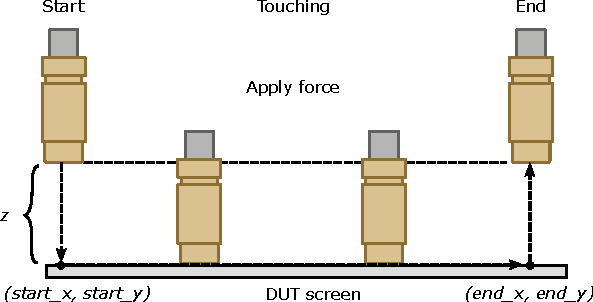
\includegraphics{drag_force_open_loop.pdf}
	\caption{Illustration of the open loop drag force gesture.}
	\label{fig:open_loop_drag_force}
\end{figure}

With open loop system the finger is attempted to be moved at clearance -2 mm while the voice coil current value saturates to the value that corresponds to given force. Open loop drag force gesture is illustrated in Figure \ref{fig:open_loop_drag_force}.

\begin{figure}[h]
	\centering
	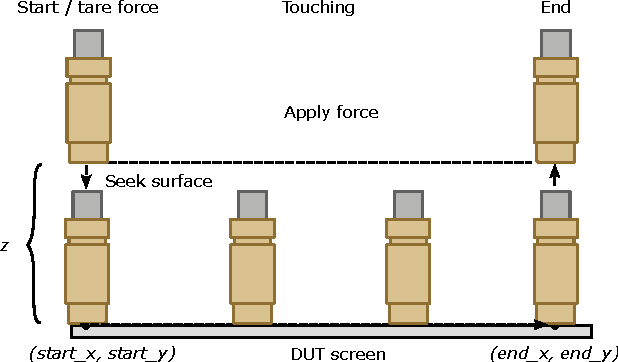
\includegraphics{drag_force_closed_loop.pdf}
	\caption{Illustration of the closed loop drag force gesture.}
	\label{fig:closed_loop_drag_force}
\end{figure}

With closed loop force, the robot first moves to base distance or given z-height and performs force tare. Then it will move the effector to touch the surface and change voice coil to force control mode. The effector will then perform normal drag motion in xy-direction while the voice coil axis applies force in closed force control loop. At the end of the drag, the control mode is changed back to position mode and the finger rises to base distance or given z-height. Closed loop drag force gesture is illustrated in Figure \ref{fig:closed_loop_drag_force}.

Following script can be used to perform drag force against DUT over DUT width applying 500 grams of force:

\begin{lstlisting}[language=Python]
from tntclient.tnt_client import TnTClient
client = TnTClient()
dut = client.dut("dut1")
dut.drag_force(x1=0, y1=dut.height/2, x2=dut.width, y2=dut.height/2, z=10, force=500)
\end{lstlisting}

The API works the same with open and closed loop force.

\section{Two-finger gestures}

This section describes the available gestures if the robot has at least two fingers. Usually these are performed with OptoFidelity Synchro tool which can rotate two fingers around the robot z-axis and the fingers can be synchronously separated along an axis that is perpendicular to the rotation axis.

\subsection{One-finger gestures with two-finger robot}

It is possible to use all the one-finger gestures with two-finger robot. With Synchro finger robot, it is possible to specify additional parameters to control how the gestures are performed. 

\begin{figure}[!h]
	\centering
	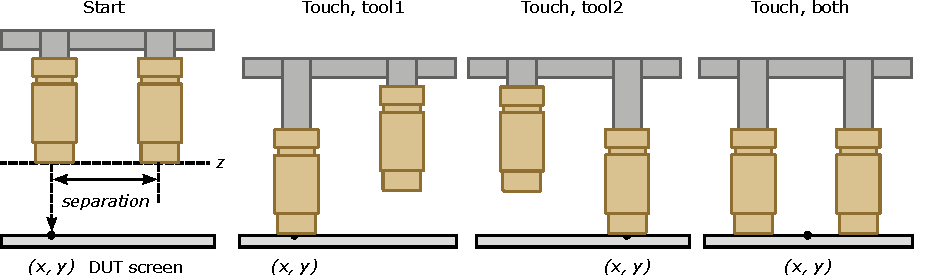
\includegraphics{two_finger_gestures.pdf}
	\caption{Illustration of one-finger gestures with two-finger robot. Notice where the target location (x,y) is in each case.}
	\label{fig:two_finger_gestures}
\end{figure}

User can give parameter \emph{separation} to specify what the finger axis-to-axis separation will be while the gesture is performed. This usually only matters if both finger effectors are used during the gesture. If the parameter is not given, a default separation value is used. This is normally the home separation.

With parameter \emph{tool\_name}, user can specify which finger is used to perform the gesture. Valid values are "tool1", "tool2" and "both". Default value is "tool1" corresponding to the default finger in the Synchro tool. With value "tool2" the second finger performs the tap motion and by default the second finger is moved over the specified location. With value "both" both fingers perform the gesture simultaneously (e.g. tap becomes two-finger tap). In that case the mid point between the two fingers is moved over the given tap location.

It is also possible to specify parameter \emph{kinematic\_name} to control which kinematics is used to plan the motion. Currently this is only implemented for the tap gesture. Valid values are "tool1", "tool2", "mid" and "synchro". This essentially means that user can control which point on the robot is moved to the location specified by the gesture coordinates. Value "tool1" moves the first finger, value "tool2" moves the second finger, value "mid" moves the mid point between the fingers and value "synchro" moves the mount point of the Synchro tool. This parameter makes it possible to e.g. tap with both fingers but let the tap location be specified with finger 1 instead of the mid point which is the default in the absence of \emph{kinematic\_name}. Figure \ref{fig:two_finger_kinematic_name} and the script below illustrate such use case.

\begin{figure}[!h]
	\centering
	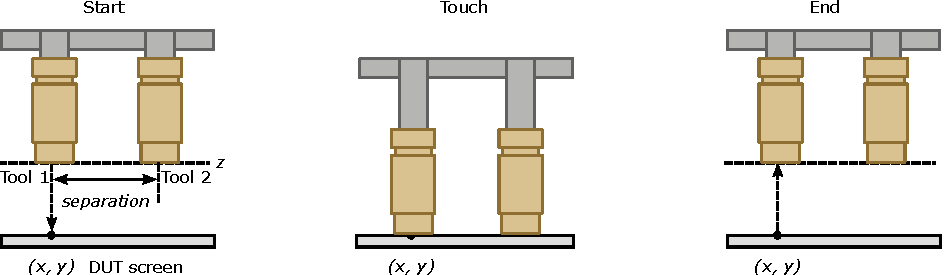
\includegraphics{two_finger_kinematic_name.pdf}
	\caption{Illustration of performing tap with \emph{kinematic\_name} "tool1" and \emph{tool\_name} "both".}
	\label{fig:two_finger_kinematic_name}
\end{figure}

\begin{lstlisting}[language=Python]
from tntclient.tnt_client import TnTClient
client = TnTClient()
dut = client.dut("dut1")
dut.tap(x=dut.width/2, y=dut.height/2, separation=60, tool_name="both", kinematic_name="tool1")
\end{lstlisting}

These gestures and parameters are illustrated in Figure \ref{fig:two_finger_gestures}.

\warningbox{When using two-finger gestures or one-finger gestures with the second or both fingers, make sure that both fingers have tip attached. Also the software book-keeping of attached tips must match reality. Otherwise there is risk of collision. See Figure \ref{fig:two_finger_collision} for illustration.}

\begin{figure}[!h]
	\centering
	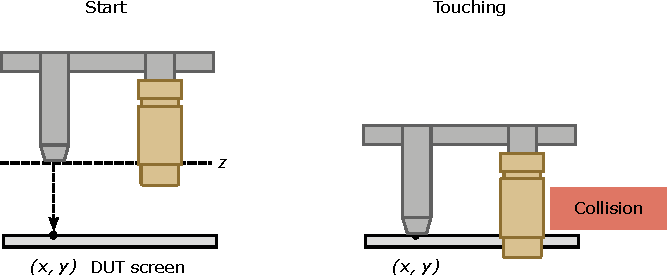
\includegraphics{two_finger_collision.pdf}
	\caption{Illustration of possible collision with two-finger robot if asymmetric tip configuration is used.}
	\label{fig:two_finger_collision}
\end{figure}

\subsection{Pinch}

In pinch gesture, the mid point between the two fingers is moved over given xy position so that both fingers are at specified z-coordinate or base distance. After that both fingers are moved at given clearance to touch the DUT surface. Then the fingers move from given start separation \emph{d1} to end separation \emph{d2}. Finally both fingers are lifted to the given z-position or base distance. Pinch gesture is illustrated in Figure \ref{fig:pinch}.

Notice that this gesture can perform \emph{pinch} and \emph{zoom} type motions depending on the given separation parameters.

\begin{figure}[h]
	\centering
	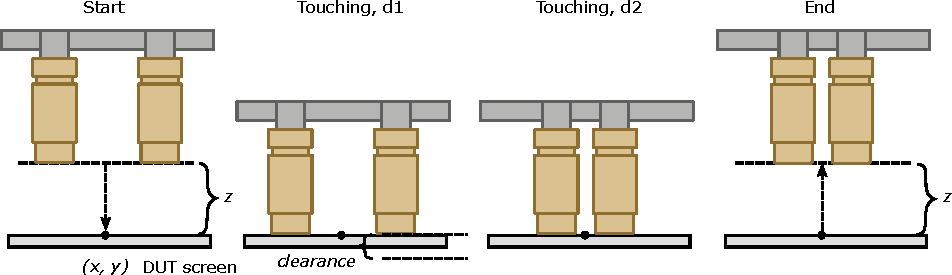
\includegraphics{pinch.pdf}
	\caption{Illustration of the pinch gesture.}
	\label{fig:pinch}
\end{figure}

Following script can be used to perform pinch over DUT from separation 60 mm to 30 mm at the center of DUT using azimuth angle 45 degrees:

\begin{lstlisting}[language=Python]
from tntclient.tnt_client import TnTClient
client = TnTClient()
dut = client.dut("dut1")
dut.pinch(x=dut.width/2, y=dut.height/2, d1=60, d2=30, azimuth=45)
\end{lstlisting}

\subsection{Rotate}

In rotate gesture, the mid point between the two fingers is moved over given xy position so that both fingers are at specified z-coordinate or base distance. After that both fingers are moved at given clearance to touch the DUT surface. Then the fingers rotate from given \emph{azimuth1} angle to \emph{azimuth2} angle. Finally both fingers are lifted to the given z-position or base distance. Rotate gesture is illustrated in Figure \ref{fig:rotate}. 

\begin{figure}[h]
	\centering
	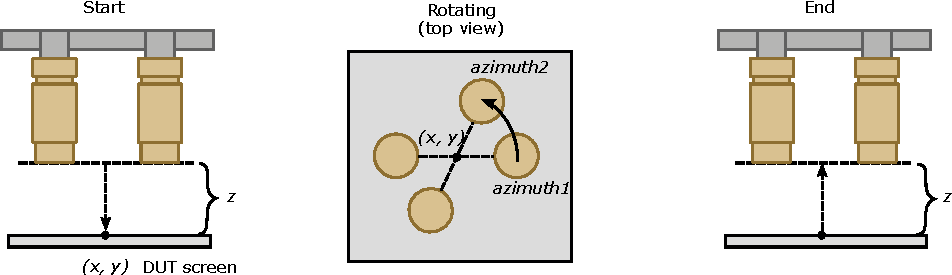
\includegraphics{rotate.pdf}
	\caption{Illustration of the rotate gesture.}
	\label{fig:rotate}
\end{figure}

Following script can be used to perform rotate gesture over DUT from azimuth angle 0 degrees to azimuth angle 90 degrees at the center of DUT using separation 60 mm:

\begin{lstlisting}[language=Python]
from tntclient.tnt_client import TnTClient
client = TnTClient()
dut = client.dut("dut1")
dut.rotate(x=dut.width/2, y=dut.height/2, azimuth1=0, azimuth2=90, separation=60)
\end{lstlisting}

\chapter{Additional robot functions}
This chapter describes additional model-dependent robot functionality that is not included in DUT gestures, for example.

\section{Surface probing}

The purpose of surface probing is to automatically detect the z-coordinate of any flat surface of interest within the robot workspace. It is particularly useful in DUT positioning. During the automatic sequence, the robot will move downwards towards the surface using the z-axis in discrete incremental steps. Surface contact is detected when the extended voice coil is pushed back sufficiently from the probing position. Once the surface has been found, the robot z-axis moves back up to the initial position and the voicecoil returns to its home position. Please see Figure~\ref{fig:surface_probing} for an illustration of the different phases.

Surface probing uses three parameters to configure the detection sequence. Parameter \emph{robot\_probing\_step} sets the size of movement when moving down step-by-step. The amount that the voicecoil actuator is extended from the neutral resting position is set with the parameter \emph{voicecoil\_probe\_position}. Finally, the required compression of the voicecoil for surface contact detection is set with \emph{surface\_detection\_threshold}.

Note, that the parameters must satisfy the conditions
\[ x_{pp} > x_{th} \text{ and } x_{ps} < 0.9 \cdot x_{pp} \text{,}\]

where $x_{pp}$ is \emph{voicecoil\_probe\_position}, $x_{th}$ is \emph{surface\_detection\_threshold} and $x_{ps}$ is \emph{robot\_probing\_step}. The detection criteria for surface contact is simply
\[\Delta x_{pp} > x_{th} \text{,}\]

where $\Delta x_{pp}$ is the change from the initial voicecoil probing position.

\warningbox{During probing there is a risk of collision with other robot workspace items. Make sure the extended probing finger is the first one to make contact and no other rigid non-compliant part of the robot accidentally collides with e.g. a finger tip rack.}

\notebox{Probing with a standard multifinger is not supported. However, custom tools that use similar dual-finger mounting as a multifinger can be used in probing, as long as the attached tool is completely rigid.}

\begin{figure}[htb]
	\centering
	\begin{overpic}[percent, tics=5]{surface_probe.pdf}
		\put(41, 43){$x_{pp}$}
		\put(65, 46){$x_{ps}$}
		\put(94, 29.5){$\Delta x_{pp}$}
		
	\end{overpic}
	\caption{Illustration of surface probing sequence in DUT positioning}
	\label{fig:surface_probing}
\end{figure}

To enable surface probing functionality and configure the parameters, add the following lines to the server configuration file and adjust the probing parameter values if needed:

\begin{lstlisting}
- name: surfaceprobe
  cls: NodeSurfaceProbe
  parent: ws
  connection: ws
  arguments:
    robot: Robot1
  properties:
    surface_probe_settings:
      robot_probing_step: 6
      voicecoil_probe_position: 9
      surface_detection_threshold: 0.5
\end{lstlisting}
\chapter{Human simulated performance testing (HSUP)}
\label{sec:HSUP}

Human simulated performance (HSUP) testing is used to measure the performance of smart devices in human-like operation. It uses high-speed camera to track visual changes in the display while the device is operated by a robot.

HSUP consists of three distinct measurement / analysis types: Watchdog, scroll performance analysis (SPA) and pen-to-ink (P2I) analysis. These are described in more detail in sections below.

\begin{figure}[!h]
	\centering
	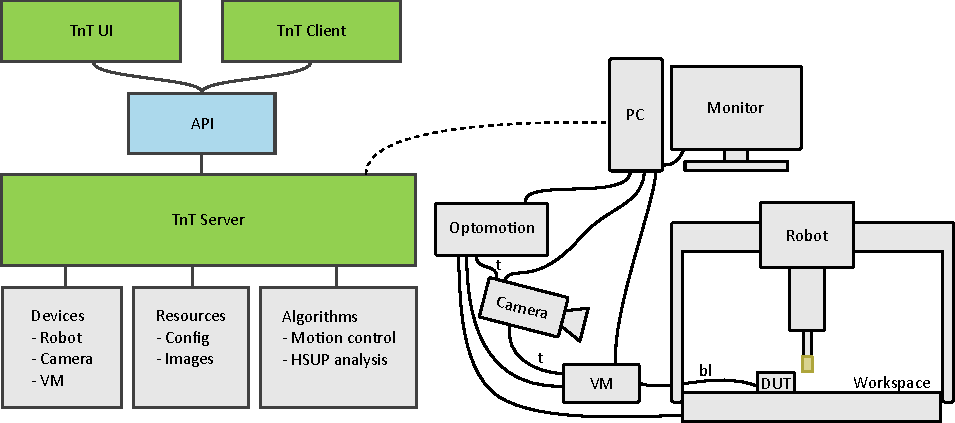
\includegraphics{hsup_sw}
	\caption{HSUP software components and hardware. Trigger signals are denoted by \texttt{t} and backlight synchronization signal is denoted by \texttt{bl}. The boxes under TnT Server denote the parts in server that are relevant for HSUP.}
	\label{fig:hsup_sw}
\end{figure}

The software components and hardware setup is illustrated in Figure \ref{fig:hsup_sw}. In HSUP, an external high speed camera is used to track changes on the DUT when robot performs some gesture. TnT Client or TnT UI are used to request an HSUP measurement and analysis. TnT server then commands the robot to perform the motion and collects any images received from the camera. The images are analyzed and stored to image database on the disk and the analysis results are stored to memory. The results can then be obtained from the server as a separate request once the measurement and analysis are complete. It is also possible to request server to analyze the stored images later.

TnT UI provides an HSUP page to set various camera parameters and quickly test the measurements. To get the measurements to work correctly for the first time, some amount of experimentation with the parameters is usually required. The obtained parameters can be saved to a configuration file and used later in scripts via TnT Client. The HSUP page cannot currently be used to command robot movements for HSUP measurements. Instead user must use TnT Client or the Sequence generator page to specify the required movements.

In HSUP the camera capture process is not triggered by software but instead direct hardware triggering is used to get exact timing between motion and image capture. There are two alternative ways to implement the triggering based on whether also synchronization to DUT backlight is required: 1) No backlight synchronization. Optomotion triggers the camera based on voice coil axis encoder change. 2) Backlight synchronization is required. OptoFidelity proprietary Video Multimeter (VM) is used to trigger the camera. Triggering is based on signal from voice coil encoder and a backlight sensor that is attached to the DUT screen. TnT Server is connected also to VM to set triggering parameters.

\section{HSUP in TnT UI}

HSUP measurement and analysis can be performed using TnT UI. It has "HSUP" page which contains controls for each measurement type as shown in Figure \ref{fig:ui_hsup}.

\begin{figure}[h]
	\centering
	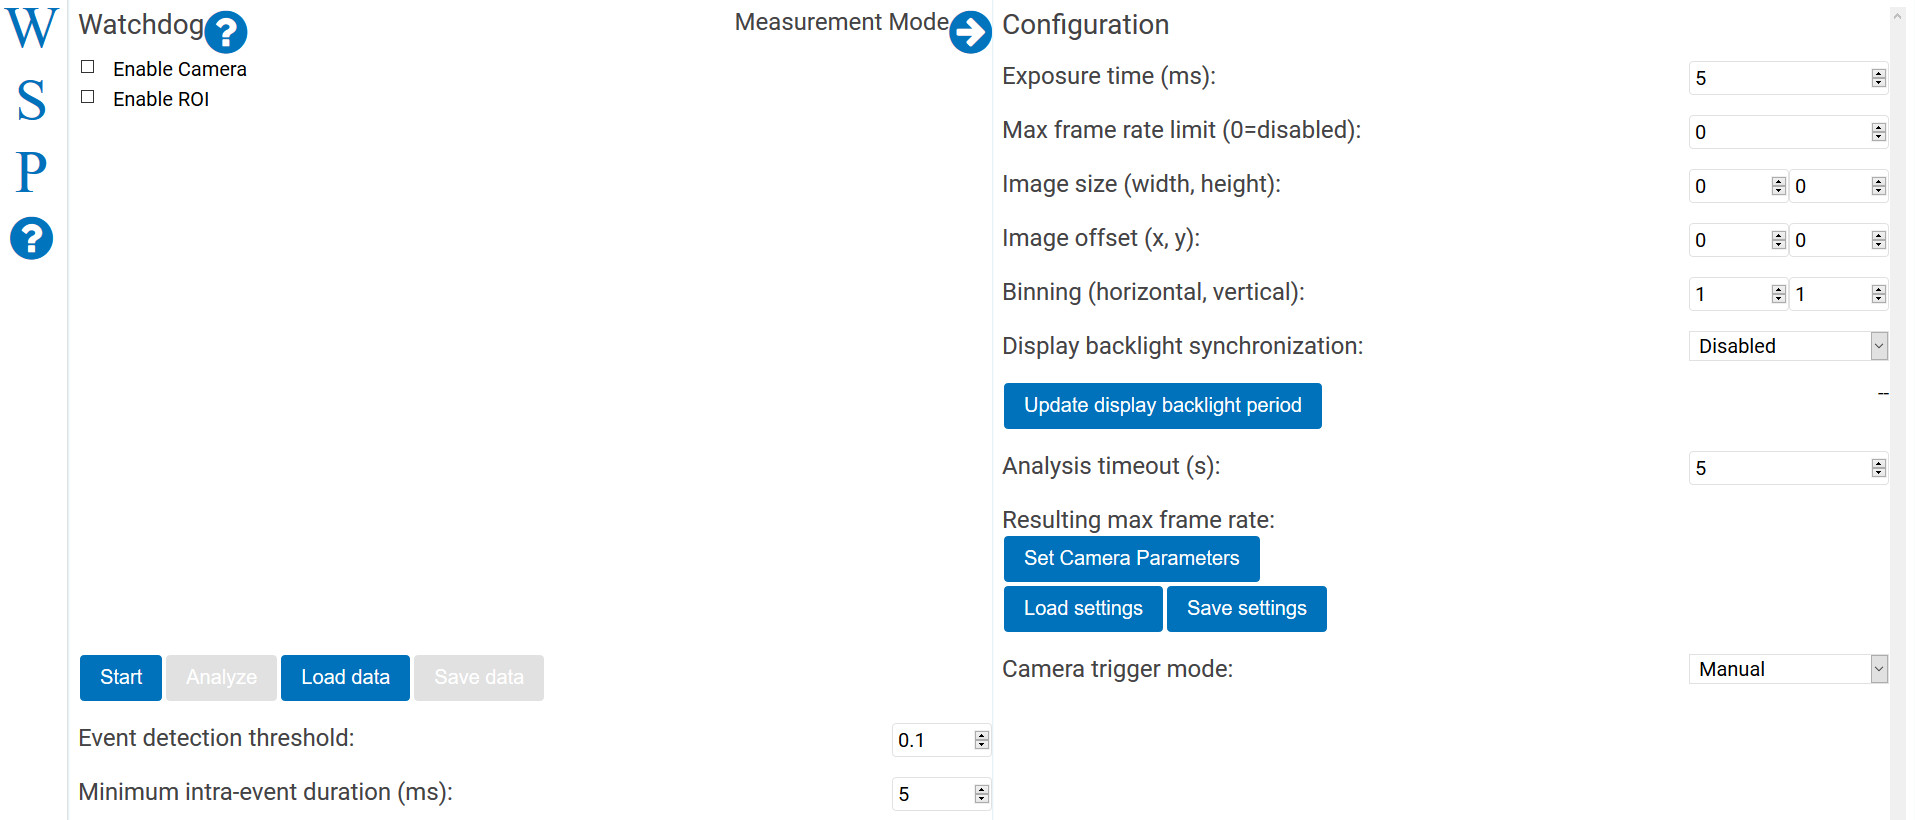
\includegraphics[width=0.9\linewidth]{ui_hsup.jpg}
	\caption{HSUP page in TnT UI.}
	\label{fig:ui_hsup}
\end{figure}

\input{from_ui_repo/hsup_common}

\input{from_ui_repo/hsup_watchdog}

\input{from_ui_repo/hsup_spa}

\input{from_ui_repo/hsup_p2i}

\section{HSUP via TnT Client}

HSUP measurements and analysis can also be run from Python scripts by use of TnT Client. See the TnT Client API reference guide for more details and the example script in the client Python package.

\importantbox{If you are using HSUP via Client, make sure that the HSUP camera is not open in TnT UI. Having the camera open in more than one instance might interfere with script execution.}
\chapter{Human simulated functional testing (HSUF)}

Human simulated functional testing (HSUF) consists of use of camera to detect icons or perform optical character recognition (OCR) and then use
robot to perform movements according to detection results. A typical use case is to find an icon on DUT screen with camera and then perform tap gesture on detected location of the icon.

\importantbox{If you are using HSUF via TnT Client, make sure that the camera is not open in TnT UI. Having the camera open in more than one instance might interfere with Client script execution.}

\section{Screenshots}

When user performs OCR or icon detection via TnT Client, the robot will move the camera over the designated DUT so that the DUT center appears at the center of the camera and the DUT surface is at the focal point of the camera. In case the DUT is rotated with respect to the camera view, the image is automatically rotated in software and cropped so that the DUT appears upright. This image is referred to as the \emph{screenshot}. See Figure \ref{fig:screenshot} for illustration.

\begin{figure}[h]
	\centering
	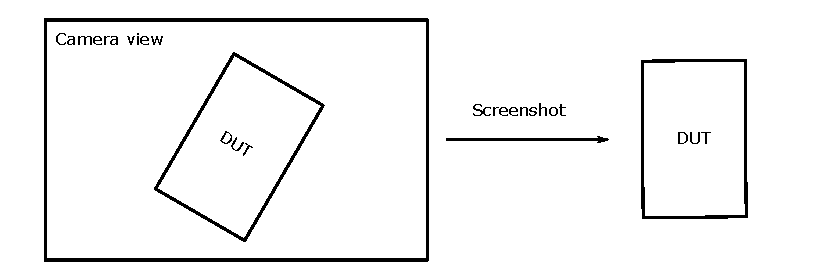
\includegraphics[width=\linewidth]{screenshot.pdf}
	\caption{Taking a screenshot of DUT with camera.}
	\label{fig:screenshot}
\end{figure}

In usual robot systems the positioning camera is attached to the z-axis of the robot and cannot rotate. Nevertheless DUTs in the workspace don't have to be aligned in any specific way in order to do functional testing due to aforementioned image transformation. 

OCR and icon detection is then applied on the screenshot image. See the docstring \texttt{TnTDutClient} \texttt{.screenshot()} for detailed description of the available parameters.

Note that the DUT must fit within the camera view in order to effectively perform functional testing. The system does not automatically try to scan over large DUT to find objects although it is possible for user to implement such behaviour by using specific offset parameters in TnT Client. In typical configuration where the camera is fixed to the robot z-axis, the robot must move between each detection and gesture which takes some amount of time. If the robot has a rotating tool, it is automatically rotated away from the camera view when taking a screenshot.

User can use TnT Client to take a screenshot of a DUT. The image is stored in TnT Server and can then be accessed via the client to perform additional tasks. User can perform OCR and icon detection on the image, do image manipulation such as cropping and color inversion or implement custom detection algorithms. Note that usually cameras have a limited capture frequency depending on resolution, connection interface and cost. Often the frame rate is as low as 5 frames per second so implementing e.g. blink detection might not be possible even though the API makes it possible in theory. Some cameras support hardware binning which can be used to downscale the camera image and hence improve the frame rate.

\section{Optical character recognition}
TnT Server implements OCR by relying on third-party libraries. These are implemented as \emph{drivers} so that user
can select appropriate OCR driver for specific use cases. Some drivers perform better that others in different use cases.
Currently following drivers are supported:
%
\begin{itemize}
\item ABBYY
\item Tesseract
\end{itemize}

ABBYY requires a commercial license, which is included in functional tester (HSUF) deliveries by default, unless agreed otherwise. Tesseract uses an open source license.

OCR can only be used via TnT Client API to create user specific test scripts. There are two APIs for finding text: \texttt{TnTDUTClient.search{\_}text()} and \texttt{TnTImageClient.search{\_}text()}. The first API method takes a screenshot as described above, saves the image file and perform OCR on the image. The OCR results i.e. the detected locations of text objects are returned in mm units in DUT context. These results can then be directly used in gesture API to perform e.g. a tap gesture on the detected location. The latter API method can be used on an existing image resource to find text on the image.

All provided OCR drivers are sensitive to defects in the image. These defects are basically anything other than text including
noise, reflections from the screen, background images, moire etc. The drivers tend to perform poorly without any filtering.
For example Tesseract is designed to find dark text on light background. If the opposite is true for the target image, user should invert the colors before performing OCR. In order to apply filtering, the \texttt{TnTDUTClient.search{\_}text()} has filter parameter that
can be used to specify an existing image filter script before OCR is performed. With \texttt{TnTImageClient.search{\_}text()}, user can
first call \texttt{TnTImageClient.filter()}. This is what also \texttt{TnTDUTClient.search{\_}text()} calls under the hood if filter parameter is given.

The filters are Python files located under \texttt{data/image{\_}filters} directory under TnT Server installation. The filter parameter
of \texttt{TnTDUTClient.search{\_}text()} is the name of a file in that directory without extension ".py". For example:

\begin{lstlisting}[language=Python]
dut = TnTDUTClient("mydut")
results = dut.search_text("Hello world!", filter="ocr")
\end{lstlisting}

The rationale that filters are stored under such location is as follows: \texttt{data} is considered to be customer specific. If
a new version of TnT Server is installed, the data directory is always retained from previous installation. The image processing
scripts may change in future revisions as we discover better ways to improve filtering for OCR. However, any changes may
break existing customer test cases as they might perform worse in specific scenarios. This approach by default retains compatibility.

When performing OCR, following things should be considered:

\begin{itemize}
\item There should be no significant reflections from the DUT visible in the camera image over the text to be detected. Even changes in background gradient due to reflections can affect the results.
\item The camera exposure and gain should be adjusted so that the text is not over nor under exposed.
\item If possible, the image should be cropped so that there is not much additional content in the image. Especially ABBYY gets confused by additional graphics and might not find anything until the image is cropped around the text.
\item Tesseract is designed to find dark text over white background. Invert image colors if this is not true for the original image. Most often in smart device testing the colors need to be inverted.
\item Text should appear upright in the screenshot image. Rotated text is usually not detected.
\item ABBYY does not give a score for the detected results. If no text pattern is provided for OCR, the score will be 1.0 for all found results. If pattern is given, it is matched against ABBYY results and a score is computed based on this matching.
\item Both ABBYY and Tesseract can fail to detect text in some circumstances. Sometimes it is necessary for user to write trial-and-error heuristics on top of the provided API to perform well in the user specific test cases.
\item The OCR drivers have certain limits for the size of text in pixels. Tesseract can usually only recognize characters of height 10 px - 30 px. User may need to rescale screenshots if the text size falls out of this range.
\item Background image behind the text may reduce the reliability of OCR.
\end{itemize}

\section{Icon teaching}

Icon teaching is usually done manually by cropping images from camera view using TnT UI. See Section \ref{sec:ui_icon_teaching} for more information.

It is also possible to teach icons from existing image files using Python and TnT Client.

\section{Icon detection}

TnT Server implements icon detection based on third-party Halcon software package. Halcon requires a commercial license, which is included in functional tester (HSUF) deliveries by default, unless agreed otherwise.

The icon detection has actually two distinct parts: 1) Icon teaching and 2) icon detection. 

The first part is done before-hand. An image is converted into a shape model which is then stored and used in the actual icon detection. The parameters used in the shape model generation affect how well the icon will be detected in various circumstances. For example how many different scalings and rotations of the icon can be detected. Currently these parameters are fixed according to our experience on icon detection in smart device functional testing.

The second part consists of taking an image (usually with a camera attached to the robot) and detecting an icon using the existing shape model. The second part can only be performed via Python scripts using TnT Client. See \texttt{TnTDutClient.find\_objects()} and its docstring for the possbile parameters that can be used in icon detection. This method works similar to the OCR counterpart i.e. it takes a screenshot and then detects icon from the resulting image. To detect icons directly from existing image, see \texttt{TnTImageClient.find\_objects()}. See also example scripts under \texttt{tntclient/examples} in the TnT Client Python package.

Icon detection tends to be very sensitive to differences between the image that was used to teach the icon and then the image where the icon is attempted to be found. Following things should be considered:

\begin{itemize}
\item Use the same camera exposure and gain when teaching the icons and when detecting the icons. This is not enforced by default so user must provide \texttt{exposure} and \texttt{gain} parameters to the icon detection API.
\item Teaching icons from ideal reference images is possible via TnT Client but it might not work in detection if the icon appears differently scaled and colored in the camera image during detection.
\item Make sure that the lighting conditions in the test area are the same when teaching icons and when detecting icons.
\item There should be no significant reflections from the DUT visible in the camera image when detecting icons.
\item Icon taught in upright orientation might not be detected with good confidence if it appears rotated in the screenshot.
\item If icon appears on the camera image at different scale than in the taught model, it might not be recognized. Usually icons sizes 1x and 2x of the taught icon are found with good confidence.
\item Cropping screenshot around icon to be detected may also help in case the icon is not detected from the entire image.
\end{itemize}

\subsection{Colored icon detection}

Halcon builds a contour shape model of the icon which does not consider color in any way. By default, icon detection does not take the color into account. However the original icon image is also stored in addition to the shape model and this can be used to take color into account. The idea is that once the icon shape is found with Halcon, a color comparison algorithm is used to weight the Halcon score based on the color similarity. Hence it is possible to distinguish icons that have the same shape but different color.

In order to enable color comparison, TnT Server configuration file must have color comparison method specified:

\begin{lstlisting}[language=Python]
- name: halcon
  cls: TnT.Detector
  parent: detectors
  connection: detectors
  arguments:
    driver: Halcon
    color_cmp_method: template
    color_cmp_params:
      threshold: 0.2
\end{lstlisting}

Comparing the color between two images is not always simple. Therefore there are multiple color comparison methods available. The best one should be selected based on particular use case. Possible methods are \texttt{template}, \texttt{histogram} and \texttt{moments}. For each method certain parameters can be given to adjust the behavior of the algorithm. Each method accepts \texttt{threshold} parameter in range [0, 1] which clamps intensity below threshold to zero. This can be effective to remove colored dark background gradient from biasing the color comparison.

\chapter{Touch panel performance testing (TPPT)}

In touch panel performance testing (TPPT) robot is used to measure the performance of individual touch panels or touch panels integrated to smart devices. Robot performs gestures such as tap and swipe on prescribed positions on the touch panel and the reported coordinates are compared to the accurately known robot coordinates.

Test parameters and test execution are defined by TPPT scripts which are run via TnT UI that provides graphical interface for setting parameters and viewing test progress. Test parameters and results are saved to SQL database (normally SQLite file). The database can then be loaded by TPPT Analysis software which calculates various metrics from the data and presents pass / fail results based on given criteria. Figure \ref{fig:tppt_sw} illustrates the relation between different software components in TPPT.

\begin{figure}[!h]
	\centering
	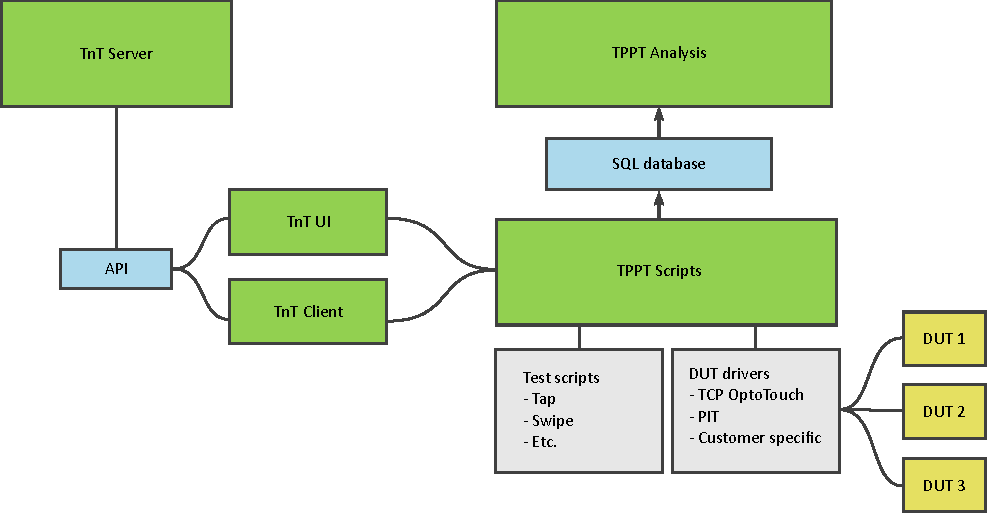
\includegraphics{tppt_sw.pdf}
	\caption{TPPT software overview.}
	\label{fig:tppt_sw}
\end{figure}

\section{TPPT scripts}

TPPT Scripts are Python files that are executed by TnT UI. The UI is used to set script parameters and to control and visualize the script execution.

\subsection{Test script structure}

TnT UI can be used to load and run test scripts. The UI provides an environment where user can give inputs to the test script and the script can easily update its progress, status, indicators etc. It offers a good control over the test scripts.

The scripts define a Context class that is instantiated when the UI loads the scripts. This context consists of all data required to run test cases including TnT Client object, settings, DUT information, tip information, test cases, database session and device driver objects.

Test scripts define a node hierarchy that is visible to the UI as a hierarchy of graphical widgets such as numeric inputs and checkboxes. Each node can define a list of Control objects, which define initial values and valid value ranges for corresponding widgets that are displayed by the UI.

\begin{figure}[!h]
	\centering
	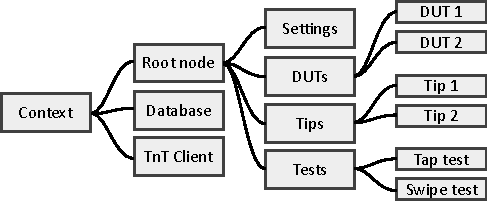
\includegraphics{tppt_node_tree.pdf}
	\caption{TPPT script structure. Each box represents a Python class object.}
	\label{fig:tppt_node_tree}
\end{figure}

The default script implementation divides nodes under Settings, DUTs, Tips and Tests nodes. Each DUT and tip is then also a node under DUTs node and Tips node respectively. Test cases are also defined as nodes under Tests node. The structure is illustrated in Figure \ref{fig:tppt_node_tree}.

Test cases are special TestStep nodes in the sense that they must implement \texttt{execute()} method that is called when the test is to be executed. The test case node class initialization is responsible for defining the controls that show up as widgets in the UI when the script is loaded.

The default script implementation implements \texttt{execute()} method in Context class that loops through all tips, DUTs and test cases that are enabled by the UI. However, utilizing the existing nodes and by writing new ones, it is possible to construct more versatile test sequences that are represented by more complex tree structure.

\subsection{Script context}

Scripts define Context class that stores all necessary data and state for running test sequences. The UI creates an instance of this class when the script is loaded and the class exposes methods for communicating information
between UI and scripts.

Script developer can easily extend and modify the widgets shown in the UI. The parameters member of Context class is a list of key-value pairs that appear in the UI as text input boxes. In the default implementation there are parameters Program, Manufacturer, Version, Operator, Serial and Notes. The values of these parameters are saved to the database.

Script developer can also easily expose button widgets in the UI by adding items to callables member of the Context class. These items are tuples (function, label) where function is a function object defined by script and label is a string used to label the button in UI.

The context object is passed down to test case initialization so that test execution can access the context resources such TnT Client object. Context also exposes indicators member, which can be used by test cases to update test progress in the UI. Indicators basically constitute an HTML element. For a more graphical progress indication, context exposes \texttt{add\_dut\_point(x, y, from\_taplike, expected)} method that can be used by a test case to visualize a touch event and expected points for tap like tests. Expected lines for swipe like tests can be visualized with \texttt{draw\_dut\_expected\_line(start\_x, start\_y, end\_x, end\_y)} method that is also exposed by context.

\subsection{Test case development}

Test cases are nodes in the tree hierarchy. They are classes that inherit the TestStep class. Test case class must define \texttt{execute()} method that is called when test case is executed once sequence is started from the UI and the test case has been enabled. Test case must also implement \texttt{visualize\_grid(dut)} method that returns \texttt{GridVisContainer} object. This method is called when UI is commanded to show points and lines that robot will execute.

Example test case:

\begin{lstlisting}[language=Python]
class MyTestCase(TestStep):

	def __init__(self, context):
		super().__init(“My test case”)
		
		# Show number input field in UI for this test case node
		self.controls.NumPoints = 5
		self.controls.info[“NumPoints”] = {“label”: “Number of points to tap”}

	def execute(self):
		# Add statements to drive robot, collect touch events and save data

	def visualize_grid(self, dut):
		return GridVisContainer(self.__class__.__name__, (dut.width, dut.height), 
		self.create_grid(dut), dut.name)
\end{lstlisting}

\input{from_ui_repo/script.tex}

\section{TPPT analysis}

TPPT Analysis is a standalone application with a web UI. It loads SQL database file produced by execution of TPPT scripts and analyses the results stored therein. Sections below give a detailed description of how to use TPPT Analysis and what kind of results are calculated from the data.

\subsection{Installation}

Installation can be done by running the installation package.

It is required that TPPT scripts are installed before TPPT Analysis can be successfully executed. TPPT Analysis requires configuration file and SQL database file from TPPT script installation.

\subsection{Windows}

The installer is a self-contained exe file which launches a wizard that will help the user through the installation process.

In case the user wants to re-install TPPT Analysis, the following procedure should be followed:
%
\begin{enumerate}
	\item Go to the folder "\tntRootPath" and create a back-up of existing "\tntTPPTAnalysisFolder" folder by renaming the folder as "TPPT Analysis 2020-01-02" where the date is the backup date.
	\item Run installation package as usual (the installer will create a new "\tntTPPTAnalysisFolder" folder).
\end{enumerate}

\subsection{Using TPPT analysis}

\begin{figure}[!h]
	\centering
	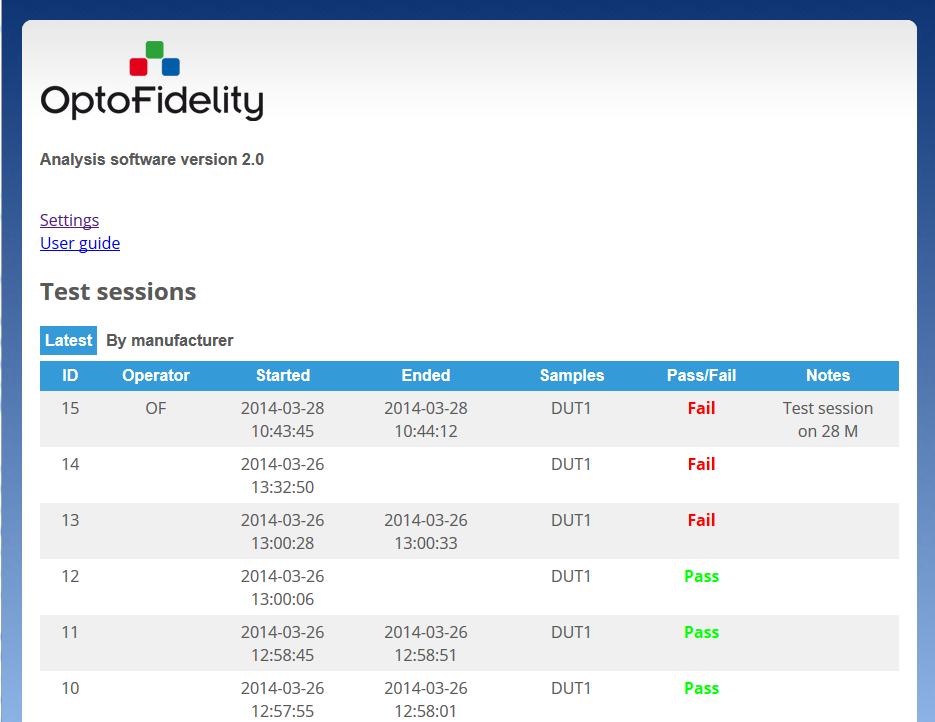
\includegraphics[width=12cm]{tppt_analysis_main_view.png}
	\caption{Analysis SW main view.}
	\label{fig:tppt_analysis_main_view}
\end{figure}

To start the analysis software, use shortcut located on desktop or navigate to \texttt{\tntRootPath\tntTPPTAnalysisFolder} and click on the icon named \texttt{\tntTPPTAnalysisExecutable}. This opens a command line prompt and a web browser. The command line prompt shows the status of the application and the browser shows the main view.

\subsubsection{Main view}

The main view is illustrated in Figure \ref{fig:tppt_analysis_main_view}. It shows the test sessions currently in the database and has two different views:
\begin{enumerate}
\item Most recent test sessions (Figure \ref{fig:tppt_analysis_recent_sessions})
\item Hierarchical tree of test sessions (Figure \ref{fig:tppt_analysis_session_hierarchy})
\end{enumerate}

\begin{figure}[!h]
	\centering
	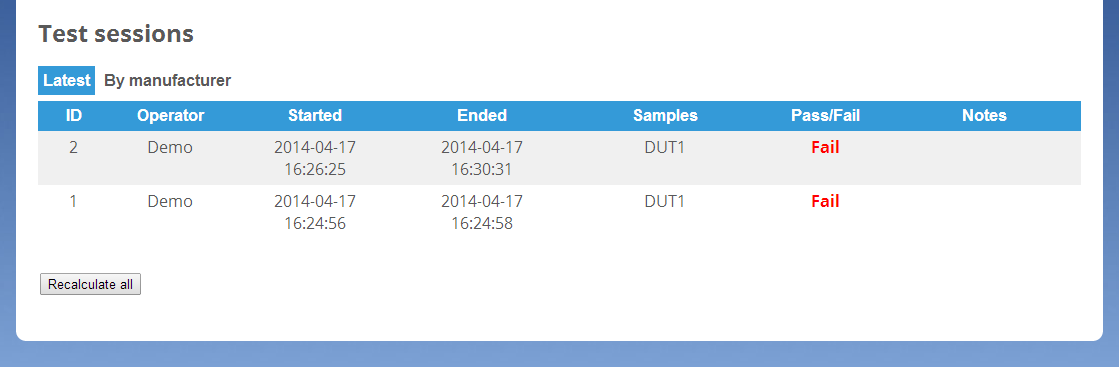
\includegraphics[width=12cm]{tppt_analysis_recent_sessions.png}
	\caption{Most recent test sessions.}
	\label{fig:tppt_analysis_recent_sessions}
\end{figure}

In addition the main view has links to global settings (see Settings view below) and recalculate all –button.

\begin{figure}[!h]
	\centering
	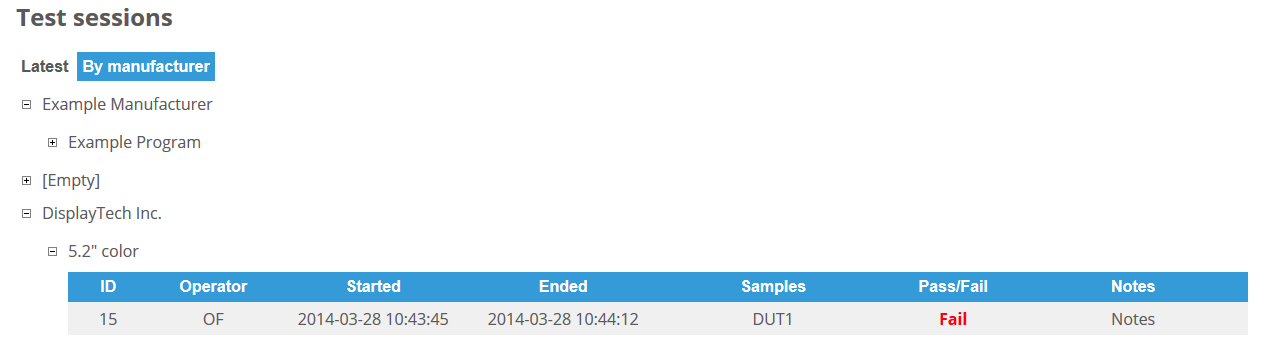
\includegraphics[width=12cm]{tppt_analysis_session_hierarchy.png}
	\caption{Hierarchical view of test sessions.}
	\label{fig:tppt_analysis_session_hierarchy}
\end{figure}

The hierarchical view shows the test sessions categorized by DUT information: Manufacturer name and Program name. The showing of the contents can be toggled by clicking the manufacturer or program name.
If there's incorrect information in the tree, like misspelled manufacturer name, that information can be corrected in DUT settings (see DUT settings view below).

\subsubsection{\label{sec:settings_view}Settings view}

In the settings view the global acceptance limits of the tests can be changed. Changing a test limit results in re-calculation of all test verdicts. 
The settings view can be accessed from the main view under the link 'Settings' as shown in Figure \ref{fig:tppt_analysis_settings_navigation}.

\begin{figure}[!h]
	\centering
	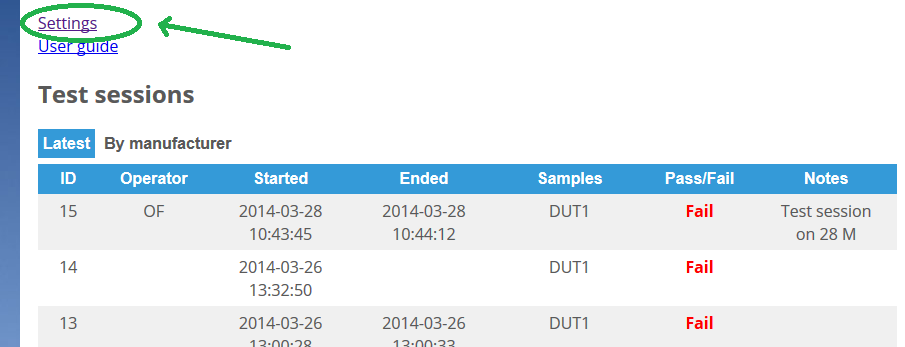
\includegraphics[width=12cm]{tppt_analysis_settings_navigation.png}
	\caption{Settings view navigation.}
	\label{fig:tppt_analysis_settings_navigation}
\end{figure}

The settings are divided to categories based on the tests they are used in ans shown in Figure \ref{fig:tppt_analysis_settings_view}. For each setting the description and the value is shown. The value can be changed by typing a new value to the field. Invalid values are marked with red field background.

\begin{figure}[!h]
	\centering
	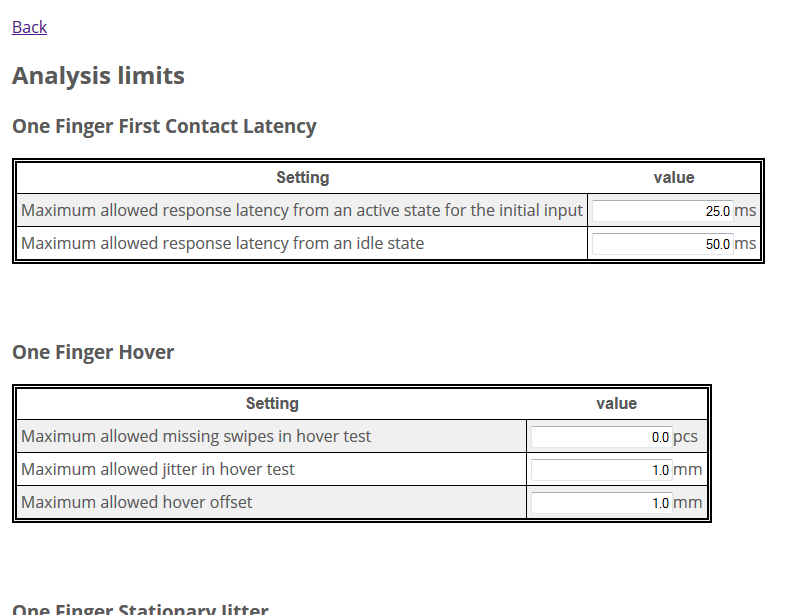
\includegraphics[width=12cm]{tppt_analysis_settings_view.png}
	\caption{Settings view.}
	\label{fig:tppt_analysis_settings_view}
\end{figure}

The save button saves the values to the database. At that time all the analysis results are recalculated, which can be a lengthy operation if there are many measurements in the database.

The descriptions of the individual tests are given in sections below starting at Section \ref{sec:one_finger_tap_test}.
Settings should not be changed when there is a test session running. In the worst case it can introduce errors to the TPPT test run.

\begin{figure}[!h]
	\centering
	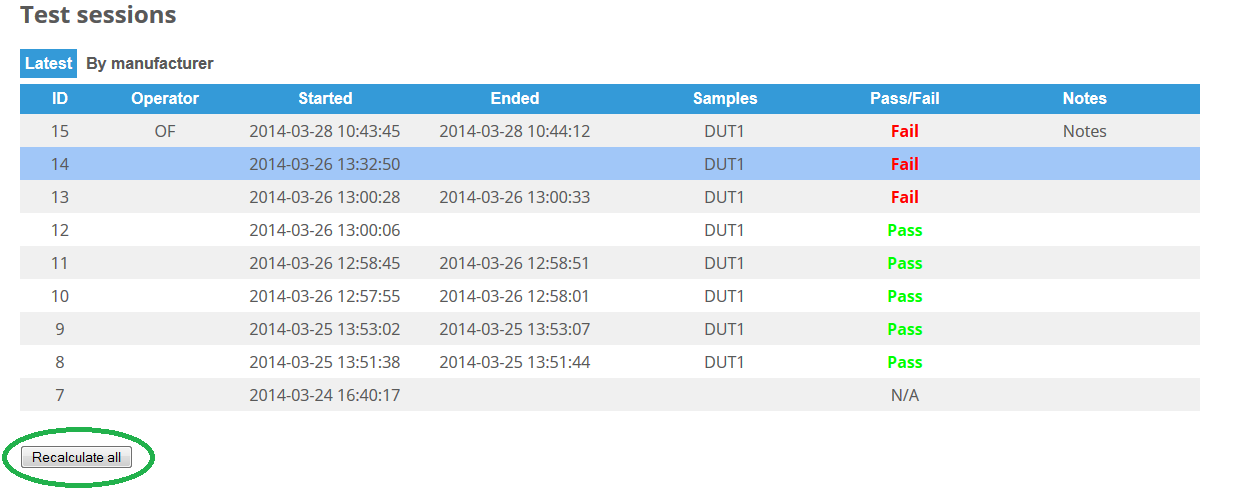
\includegraphics[width=12cm]{tppt_analysis_recalculate_all.png}
	\caption{Recalculate all.}
	\label{fig:tppt_analysis_recalculate_all}
\end{figure}

The recalculate all button (see Figure \ref{fig:tppt_analysis_recalculate_all}) recalculates all the analysis results in the database. This can take some time if there are many test sessions in the database.

\warningbox{Recalculate all should not be run when there is a test session running. In the worst case it can introduce errors to the TPPT test run and result in incorrect verdicts. If user ends up in this situation, then the results can be recalculated correctly by running Recalculate all when no tests are running.}

\subsubsection{Test session overview}

\begin{figure}[!h]
	\centering
	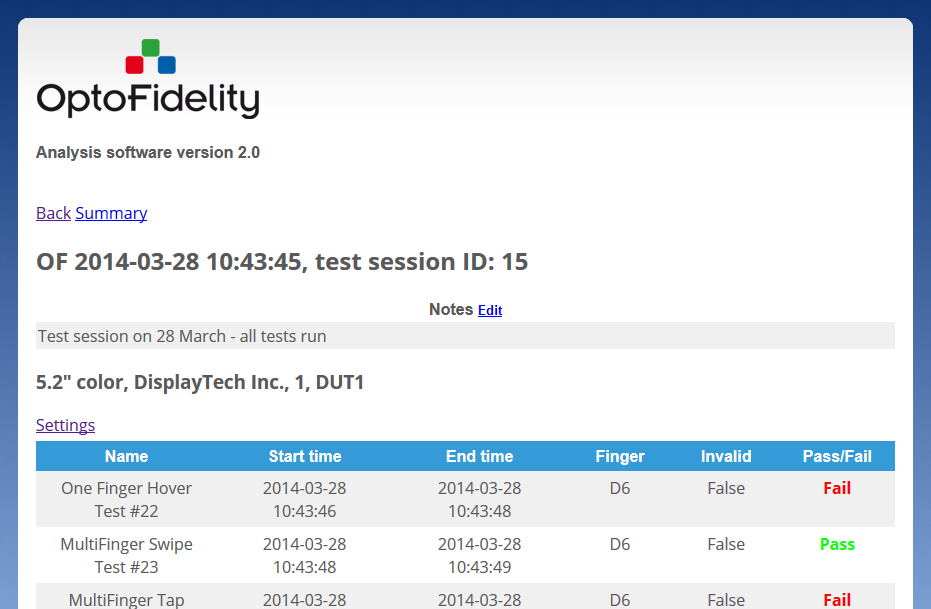
\includegraphics[width=12cm]{tppt_analysis_session_overview.png}
	\caption{Test session overview.}
	\label{fig:tppt_analysis_session_overview}
\end{figure}

The test session page can be opened by clicking a test session in the main view. The test session view shows the individual test results in a single test run. This is illustrated in Figure \ref{fig:tppt_analysis_session_overview}.
If multiple DUT functionality is enabled, the test results are grouped by DUT. Below the DUT information is link to the DUT settings (see Section \ref{sec:tppt_analysis_test_analysis})

\begin{figure}[!h]
	\centering
	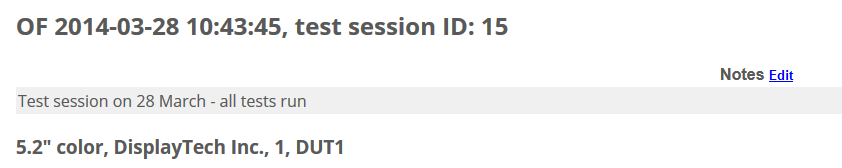
\includegraphics[width=12cm]{tppt_analysis_session_notes.png}
	\caption{Session notes.}
	\label{fig:tppt_analysis_session_notes}
\end{figure}

\begin{figure}[!h]
	\centering
	
\includegraphics[width=12cm]{tppt_analysis_session_notes_empty.png}
	\caption{Empty session notes with edit button.}
	\label{fig:tppt_analysis_session_notes_empty}
\end{figure}

At the top of the page the session notes are shown. The first words of the notes are shown also in the main page. The notes can be edited by selecting 'edit', after which the notes can be edited in the text field. The edited notes must be saved by selecting 'save'. Note editing is illustrated in Figures \ref{fig:tppt_analysis_session_notes} and \ref{fig:tppt_analysis_session_notes_empty}.

\subsubsection{DUT settings view}

\begin{figure}[!h]
	\centering
	\subfloat[DUT settings view]{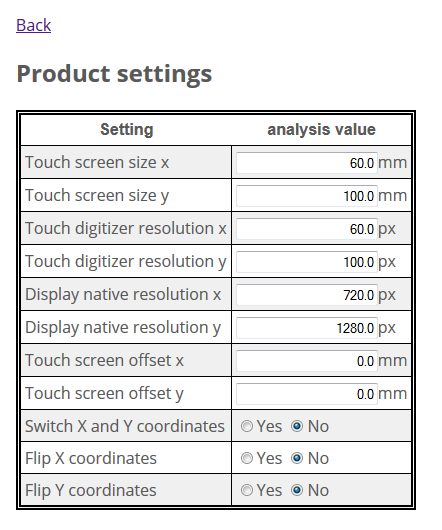
\includegraphics[width=4cm]{tppt_analysis_dut_settings_view.png}\label{fig:tppt_analysis_dut_settings_view}}
	\qquad
	\subfloat[DUT properties and save button]{\includegraphics[width=4cm]{tppt_analysis_dut_properties.png}\label{fig:tppt_analysis_dut_properties}}
	\caption{DUT settings.}
\end{figure}

The DUT settings control the characteristics of the DUT. The settings are separate for each DUT and test session. See Figure \ref{fig:tppt_analysis_dut_settings_view}. The different settings are the following:

\textbf{Touch screen size x}: width of the touch screen in millimeters.

\textbf{Touch screen size y}: height of the touch screen in millimeters.

\textbf{Touch digitizer resolution x}: touch digitizer resolution in direction of width of the screen in pixels.

\textbf{Touch digitizer resolution y}: touch digitizer resolution in direction of height of the screen in pixels.

\textbf{Display native resolution x}: display native resolution in direction of width of the screen in pixels.

\textbf{Display native resolution y}: display native resolution in direction of height of the screen in pixels.

\textbf{Touch screen offset x}: Offset of the actual panel top left from the taught top left corner of the panel in millimeters.

\textbf{Touch screen offset y}: Offset of the actual panel top left from the taught top left corner of the panel in millimeters.

\textbf{Switch X and Y coordinates}: If selected, the X and Y coordinates are exchanged. Switch X and Y-coordinates switch is used before Flip X and Y settings.

\textbf{Flip X coordinates}: Normally the positive X coordinate direction is right. If Flip X coordinates is selected, the direction is reversed (positive direction to left).

\textbf{Flip Y coordinates}: Normally the positive Y coordinate direction is down. If Flip Y coordinates is selected, the direction is reversed (positive direction up).

The Flip X, Flip Y, and Switch X and Y coordinates can be used to adjust to screen rotation. For example, if a typical display is rotated 90 degrees clockwise (positive X direction down, positive Y direction left), this can be adjusted by selecting Switch X and Y coordinates (positive Y direction down, positive X direction left) and Flip X coordinates (positive X direction right).

Below the test session related DUT settings are the DUT properties: Manufacturer name, program name, version, and Sample ID. See Figure \ref{fig:tppt_analysis_dut_properties}.

All the settings are saved by pressing 'Save all'. After the settings have been changed, the measurements in the test session are re-calculated to accommodate new settings.

\subsubsection{Test session summary}

Summary page lists all results of tests run in test session. Test session overview is in the top of the page. From each test item the general test results are shown. In order to view the detailed results, click the corresponding table row to open the full test report.

\warningbox{Test case verdict is calculated and stored to the database when test report is opened. If the test is still running, the verdict may be incorrect. This can be fixed by opening the test report again after the test is finished and the verdict can be correctly determined.}

\subsection{\label{sec:tppt_analysis_test_analysis}Common items in test reports}

\begin{figure}[!h]
	\centering
	\includegraphics[width=10cm]{tppt_analysis_common_items.png}
	\caption{Common items.}
	\label{fig:tppt_analysis_common_items}
\end{figure}

At the top of the test report page are the functions common to all test reports (see Figure \ref{fig:tppt_analysis_common_items}):

\textbf{Back}: Return to test session view.

\textbf{Analysis Home}: Return to main page

\textbf{Print}: Print the test report. 

\textbf{Load CSV}: Load the test item raw data as a CSV file.

\textbf{Note}: Use the print button in the test page rather than the browser’s print function. The print button is disabled when all the images in the report are not yet loaded.

When detailed plots (pictures) are shown in test reports, they can be toggled by the toggle buttons (see Figure \ref{fig:tppt_analysis_toggle_buttons}):

\begin{figure}[!h]
	\centering
	\includegraphics[width=10cm]{tppt_analysis_toggle_buttons.png}
	\caption{Toggle buttons.}
	\label{fig:tppt_analysis_toggle_buttons}
\end{figure}

\textbf{All}: Toggles the state of all detailed plots.

\textbf{Failed}: Toggles the state of failed plots

\textbf{Passed}: Toggles the state of passed plots

If some of the plots are manually opened and then toggle button is pressed, the plots are all either opened or closed, depending on the state of the detailed plots. The desired state can be achieved with at most two presses of the toggle button.

\subsection{\label{sec:one_finger_tap_test}One Finger Tap Test}

One Finger Tap Test report shows the results of the tap test. The tap test is used to measure the tap accuracy performance of the DUT.

\subsubsection{Settings}

The settings (see Section \ref{sec:settings_view}) related to the one finger tap test are:

\textbf{Maximum allowed positional error}: The distance from the point that the robot presses to the coordinates reported by the DUT.

\textbf{Maximum allowed missing inputs}: The maximum allowed amount of missing inputs in the test.

\textbf{Edge area distance from edge in Tap test}: The edge area width. The edge area can have different thresholds than rest of the DUT. If this setting is positive (larger than 0), the edge area analysis is enabled and the two following settings are in use:

\begin{enumerate}
\item \textbf{Maximum allowed positional error in edge area}: The maximum allowed positional error if the point that the robot presses resides in the edge area.
\item \textbf{Maximum allowed missing edge inputs}: The maximum allowed amount of missing inputs in the edge area in addition to the global value. Thus, if the global value is 1 and missing edge inputs value is 2, there can be at most 3 missing inputs in the edge area if none are missing in other parts of the DUT.
\end{enumerate}

\subsubsection{Report contents}

The detailed results are:

\textbf{Max accuracy error: Maximum accuracy error}. If edge area analysis is enabled, this is reported for both the edge area and for the rest of the display (center).

\textbf{Missing inputs}: Missing inputs in the test. If edge area analysis is in use, this is reported separately for the edge area and for the rest of the display (center).

\subsubsection{Preview images}

The first preview image illustrated in Figure \ref{fig:tppt_analysis_tap_preview} shows the overview of the DUT. Circles represent the robot points and the size of the circle is the size of the allowed area given by accuracy error. If the input is missing, the circle is drawn red. If the input is outside the allowed area, the position of the input is shown with red marker, otherwise a green marker is used.

\begin{figure}[!h]
	\subfloat[Preview]{\includegraphics[width=8cm]{tppt_analysis_tap_preview.png}\label{fig:tppt_analysis_tap_preview}}
	\subfloat[Scatter plot]{\includegraphics[width=8cm]{tppt_analysis_tap_scatter.png}\label{fig:tppt_analysis_tap_scatter}}
	\caption{Tap test.}
\end{figure}

The second image illustrated in Figure \ref{fig:tppt_analysis_tap_scatter} gives the scatter plot. It plots all the measurements in relation with the point that the robot has pressed (reference point). In the image the distribution of the tap error can be observed. The histograms on the sides show the distribution of the points on the axes. The unit in the histogram is one measured event, and the cumulative amount of events in each bar can be read from the scale of the respective histogram. If edge analysis is conducted, two acceptance circles are shown (see above).

The last image(s) give the same scatter information with limited display area. This is useful if there are erroneous measurements that are far from the reference point. With limited display area the points near the reference point can be viewed in more detail.

All the preview images can be viewed in higher resolution by clicking the preview image.

\subsection{One Finger Swipe Test}

The one finger swipe test report shows the results of the swipe test. The swipe test is used to measure the accuracy of the DUT, when the touch is in linear motion.

\subsubsection{Settings}

\begin{figure}[!h]
	\centering
	\includegraphics[width=14cm]{tppt_analysis_swipe_parameters.png}
	\caption{Swipe parameters.}
	\label{fig:tppt_analysis_swipe_parameters}
\end{figure}

The settings related to the one finger swipe test are:

\textbf{Maximum allowed offset}: The maximum allowed offset of swipe point perpendicular to the line that the robot has swiped (see Figure \ref{fig:tppt_analysis_swipe_parameters}). 

\textbf{Maximum allowed jitter}: Maximum allowed jitter in a swipe. Jitter is the peak-to-peak maximum movement perpendicular to the swipe line within a sliding window (see Figure \ref{fig:tppt_analysis_swipe_parameters} above). 

\textbf{Jitter search mask}: The width of window in mm along the swipe line in which the jitter is calculated. 

\textbf{Maximum amount of missing swipes}: A swipe is missing if no points are reported for a single swipe. If the number of missing swipes is more than the maximum amount, the test has failed.

\subsubsection{Report contents}

\begin{figure}[!h]
	\centering
	\includegraphics[width=10cm]{tppt_analysis_swipe_summary.png}
	\caption{Swipe test summary tables.}
	\label{fig:tppt_analysis_swipe_summary}
\end{figure}

The report shows the maximum offset measured in the test, maximum jitter and the amount of missing swipes. The summary table is shown in Figure \ref{fig:tppt_analysis_swipe_summary}. If these values are within configured limits, they are marked Pass. Total test verdict is Pass is all of these results are Pass. If any of them is Fail then test verdict is Fail. It is possible that maximum jitter or maximum offset are 'N/A' if there is insufficient data (less than two points per swipe). If either one is 'N/A', the test case verdict is 'N/A' if the number of missing swipes is less than the maximum allowed missing swipes. If there are more swipes missing than allowed, the test verdict is Fail regardless of jitter and offset verdicts.

Below the summary table in Figure \ref{fig:tppt_analysis_swipe_summary} there is another table showing the maximum deviation from fitted lines and the mean of maximum deviations from each fitted line. These two values don't have a verdict and hence don't directly affect the total test case verdict.

\subsubsection{Preview images}

\begin{figure}[!h]
	\centering
	\includegraphics[width=10cm]{tppt_analysis_swipe_preview.png}
	\caption{Main swipe test preview image.}
	\label{fig:tppt_analysis_swipe_preview}
\end{figure}

The main preview image illustrated in Figure \ref{fig:tppt_analysis_swipe_preview} shows the swipes and the measured points. The swipes are shown with gray arrows. The measured points are colored green or red based on their offset values – the values exceeding the maximum allowed offset are colored red. If maximum allowed jitter is exceeded, it is not shown on the preview image. A higher resolution version of the image is available by clicking the preview image on the report.

\begin{figure}[!h]
	\centering
	\includegraphics[width=10cm]{tppt_analysis_swipe_details.png}
	\caption{Swipe details.}
	\label{fig:tppt_analysis_swipe_details}
\end{figure}

In Figure \ref{fig:tppt_analysis_swipe_details} the detail table shows the maximum offset and jitter values for each individual swipe. The Pass / Fail value of a swipe is determined by the offset and jitter values and whether the swipe is missing. A swipe is missing if it has no measurement points. If a swipe has at least one point, it is not considered missing.

If the maximum offset within a swipe exceeds the configured limit, the individual swipe is Fail and also the total test verdict is Fail. If a swipe has no measurement points, the swipe offset verdict is 'N/A'. Value 'N/A' does not affect the maximum offset verdict of the entire test case, but it is treated as missing swipe.

If the maximum jitter within a swipe exceeds the configured limit, the individual swipe is Fail and also the total test verdict is Fail. If a swipe has less than two measurement values, the jitter value is 'N/A', as jitter calculation requires at least two measurement values. Value 'N/A' does not affect the maximum jitter verdict of the entire test case.

If a swipe is missing, the verdict of the individual swipe is Fail but the total test case verdict may still be Pass if the number of missing swipes does not exceed the configured limit and also offset and jitter are within limits. Hence it is possible that a test case with verdict Pass has individual swipes with verdict Fail.

The individual swipe plot images illustrated in Figure \ref{fig:tppt_analysis_swipe_details} show the measured swipe points on the left and the detailed analysis of the swipe on the right. The detailed analysis shows the offset for each point (blue) and the calculated jitter (red). The x-axis is measured along the robot swipe line. Vertical lines (gray) show the location of the measurement point in the X axis. 

\subsection{One Finger Stationary Jitter Test}

One finger stationary jitter report reports the results of the stationary jitter test. It is used to test the performance of the DUT when a single point is pressed and hold. Optimally the DUT should report a single coordinate consistently.

\subsubsection{Settings}

The one finger stationary jitter test has the following settings:

\textbf{Maximum allowed stationary jitter}: The maximum amount of jitter allowed for a single point.

\subsubsection{Report contents}

The stationary jitter reports the maximum measured stationary jitter in the test. In addition, the results for individual points pressed are measured.

The jitter is calculated from the first coordinate reported by the DUT. The jitter for each successive measurement value is the distance from the first reported point. The jitter reported for an individual tap is the maximum of jitters for individual points.

\subsubsection{Preview images}

\begin{figure}[!h]
	\centering
	\includegraphics[width=10cm]{tppt_analysis_stationary_jitter_details.png}
	\caption{Stationary jitter details.}
	\label{fig:tppt_analysis_stationary_jitter_details}
\end{figure}

The main preview image illustrated in Figure \ref{fig:tppt_analysis_stationary_jitter_details} shows the different points measured related to the DUT. Passed points (jitter value not exceeding threshold) are marked green, failed points are marked with red color. Note that the passed points are determined by the first input from the panel – the analysis does not take robot touch point into account when determining the pass/failure limits.

\subsection{One Finger Tap Repeatability Test}

The one finger tap repeatability report shows the results of the repeatability test. The tap repeatability test is used to measure the panel’s ability to report consistent coordinates when the same location of the panel is pressed repeatedly with the robot.

\subsubsection{Settings}

The settings related to the tap repeatability test are:

\textbf{Maximum tap repeatability error}: The maximum distance of the reported points either in x- or y-direction.

\subsubsection{Report contents}

The report shows the maximum repeatability errors in both x- and y-directions. The maximum errors reported may be from different measurement points. 

Individual measurement points are reported in a table with respective errors in x- and y-directions.

\subsubsection{Preview images}

The main preview image shows the passed and failed points located in the DUT. The point is passed if errors in both the x- and y-directions are less than equal to the maximum repeatability error.

\begin{figure}[!h]
	\centering
	\includegraphics[width=10cm]{tppt_analysis_tap_repeatability_details.png}
	\caption{One finger tap repeatability details.}
	\label{fig:tppt_analysis_tap_repeatability_details}
\end{figure}

The detailed images illustrated in Figure \ref{fig:tppt_analysis_tap_repeatability_details} show the location of the taps. The reference point shows the location that the robot has tapped. The inner box in the image shows the acceptance area of the measurements. The measurements outside the acceptance area are marked failed with red color. 

Note: the acceptance area is not an absolute definition, it is estimated from the measurement values. The pass/fail value is absolute, as it is calculated from peak-to-peak values of the measurements in both x- and y-directions.

\subsection{One Finger Stationary Reporting Rate Test}

The one finger stationary reporting rate test reports the results of the stationary reporting rate test. It measures the reporting frequency of the DUT.

Note: This test is platform-specific. Some platforms, like Android, do not report tap events if the tap is stationary. In those platforms the stationary reporting rate test is not applicable.

\subsubsection{Settings}

The settings related to the stationary reporting rate test are:

\textbf{Minimum allowed reporting rate}: The minimum reporting rate that is allowed. Measured in Herz (Hz).

\subsubsection{Report contents}

The report contains the minimum measured reporting rate for the test. The reporting rate is calculated from time intervals between reported coordinates from DUT. 

The detailed table shows the measured minimum and maximum reporting rate for each measured point. 

\subsubsection{Preview images}

The main preview image shows the measured points on the DUT, and marks the point passed (green) or failed (red) based on the minimum reporting rate for that specific point.

\begin{figure}[!h]
	\centering
	\includegraphics[width=10cm]{tppt_analysis_stationary_reporting_rate_details.png}
	\caption{Stationary reporting rate details.}
	\label{fig:tppt_analysis_stationary_reporting_rate_details}
\end{figure}

The detailed image illustrated in Figure \ref{fig:tppt_analysis_stationary_reporting_rate_details} shows the reporting rate for an individual tap. The X axis is the DUT event index, and the Y axis shows the delay from the previous event. The red line (if visible) shows the acceptance limit. Delays above the acceptance limit are considered failed. Note: the acceptance limit is the reciprocal of the minimum allowed reporting rate.

\subsection{One Finger Non-Stationary Reporting Rate Test}

The One finger non-stationary reporting rate test report shows the results for non-stationary reporting rate test.

Note: the applicability concerns for stationary reporting rate test do not apply for non-stationary reporting rate test.

\subsubsection{Settings}

The settings related to the stationary reporting rate test are:

\textbf{Minimum allowed reporting rate}: The minimum reporting rate that is allowed. Measured in Herz (Hz).

\subsubsection{Report contents}

The report contains the minimum measured reporting rate for the test. The reporting rate is calculated from time intervals between reported coordinates from DUT. Additionally the amount of missing lines (missing inputs) is reported.

The detailed table shows the measured minimum and maximum reporting rate for each measured point. 

\subsubsection{Preview images}

\begin{figure}[!h]
	\centering
	\includegraphics[width=10cm]{tppt_analysis_non_stationary_reporting_rate_preview.png}
	\caption{Non-stationary reporting rate preview.}
	\label{fig:tppt_analysis_non_stationary_reporting_rate_preview}
\end{figure}

The main preview image illustrated in Figure \ref{fig:tppt_analysis_non_stationary_reporting_rate_preview} shows the measured points on the DUT, and marks the point passed (green) or failed (red) based on the minimum reporting rate for that specific point. The arrows show the location and direction of robot movement.

The detailed preview image is the same than in stationary reporting rate test (see above).

\subsection{Two Finger Separation Test}

The separation test report shows the results for the separation test that is used to measure the DUTs ability to separate distinct fingers (effectors) based on their distance from each other.

\subsubsection{Settings}

The settings related to the separation test are:

\textbf{Maximum allowed finger separation distance (vertical and horizontal)}: The maximum distance in which the fingers are allowed to be interpreted as one input. If the DUT cannot detect distinct fingers with larger separation distances than the setting, the result is fail. This setting is used for horizontal and vertical finger alignments.

\textbf{Maximum allowed finger separation distance (diagonal)}: The maximum distance in which the fingers are allowed to be interpreted as one input in other directions than strictly horizontal or vertical.

\subsubsection{Report contents}

The first table lists the measured separation distances with the different separation angles. The distance measured is the first distance with which the different fingers are detected as separate fingers and all the successive tests with larger separation distances are also successful.

If the separation distance is larger than the maximum allowed setting for that angle, the measurement is marked as failed.

In the second table, all the different measurements with all angles and separation distances are listed. Individual measurement is marked as passed, if the different fingers could be detected. If an individual test fails with separation distance less or equal to maximum allowed setting, the failed test does not affect the overall result of the test.

\subsubsection{Preview images}

\begin{figure}[!h]
	\subfloat[Preview]{\includegraphics[width=8cm]{tppt_analysis_separation_preview.png}\label{fig:tppt_analysis_separation_preview}}
	\subfloat[Details]{\includegraphics[width=8cm]{tppt_analysis_separation_details.png}\label{fig:tppt_analysis_separation_details}}
	\caption{Separation test.}
\end{figure}

The first preview image of the separation test illustrated in Figure \ref {fig:tppt_analysis_separation_preview} shows the overall results for the test. It shows the individual robot positions, in which the fingers have been pressed. Each position is marked as passed or failed depending on the individual separation result.

The second image illustrated in Figure \ref{fig:tppt_analysis_separation_details} shows the analysis of the test results based on the actual detected finger events. The event positions detected as separate are marked with green color. The event positions that show only one finger id (fingers are detected as one), are marked with red color.

\begin{figure}[!h]
	\centering
	\includegraphics[width=10cm]{tppt_analysis_separation_details_2.png}
	\caption{Separation test details.}
	\label{fig:tppt_analysis_separation_details_2}
\end{figure}

The details image illustrated in Figure \ref{fig:tppt_analysis_separation_details_2} shows the received events from a single separation test with single angle and separation distance. The events are marked to the picture with red or green markers. The events having the same event id are connected by solid lines. The finger positions of the robot are marked with circles.

\subsection{Multifinger Tap Test}

Multifinger Tap Test report shows the results of the multifinger tap test. The multifinger tap test is used to measure the tap accuracy performance of the DUT when the DUT is operated with multiple fingers.

\subsubsection{Settings}

The settings related to the multifinger tap test are:

\textbf{Maximum allowed positional error}: The distance from the point that the robot presses to the coordinates reported by the DUT.

\textbf{Maximum allowed missing inputs}: The maximum allowed amount of missing inputs in the test.

Note: the edge area analysis is not supported in the current version of analysis software.

\subsubsection{Report contents}

The detailed results are:

\textbf{Max accuracy error}: Maximum accuracy error. 

\textbf{Missing inputs}: Missing inputs in the test. 

\textbf{Errors}: The errors detected while analyzing the images.

The detailed results table shows the results for individual taps. For each tap the number of fingers, errors, and maximum offset are reported. The individual test fails if the maximum offset is exceeded or there are errors in the test.

\subsubsection{Preview images}

\begin{figure}[!h]
	\subfloat[Preview]{\includegraphics[width=8cm]{tppt_analysis_multifinger_tap_preview.png}\label{fig:tppt_analysis_multifinger_tap_preview}}
	\subfloat[Details]{\includegraphics[width=8cm]{tppt_analysis_multifinger_tap_details.png}\label{fig:tppt_analysis_multifinger_tap_details}}
	\caption{Multifinger tap test.}
\end{figure}

The overview image illustrated in Figure \ref{fig:tppt_analysis_multifinger_tap_preview} shows the passed and failed mesurements on the DUT. Only the location of the first finger is reported. Thus, each point on the DUT corresponds to one tap with multifinger effector.

The detailed overview image illustrated in Figure \ref{fig:tppt_analysis_multifinger_tap_details} is similar to the overview image, but it shows additionally the all the fingers in the multifinger effector connected by a line. If the effector lines overlap, the resulting image may be difficult to interpret (see above). In these cases the detailed locations of the effector can be seen in the detailed images (see below).

\begin{figure}[!h]
	\subfloat[Scatter plot]{\includegraphics[width=8cm]{tppt_analysis_multifinger_tap_scatter.png}\label{fig:tppt_analysis_multifinger_tap_scatter}}
	\subfloat[Details]{\includegraphics[width=8cm]{tppt_analysis_multifinger_tap_details_2.png}\label{fig:tppt_analysis_multifinger_tap_details_2}}
	\caption{Multifinger tap test details.}
\end{figure}

The scatter plot illustrated in Figure \ref{fig:tppt_analysis_multifinger_tap_scatter} shows the tap locations for each of the taps and in each of the effector fingers. Only a limited version is shown, as the errors in the tap test quickly render the scatter plot non-usable.

The tap details image illustrated in Figure \ref{fig:tppt_analysis_multifinger_tap_details_2} shows one tap with multifinger effector along with the measured events from the DUT. The upper portion of the image shows the general results of the tap. The circles give the maximum position error related to the effector positions. If a point is failed, a red line connects the point to the effector position (see above). 

The small scatter diagrams show the individual finger results of the effector. For each finger, the amount of events is reported (n, e.g. for Finger 1 the amount of events is 100) and the finger id received in the event. 

Note: the finger ids can be used to detect errors. Generally the finger ids are distributed randomly between different effector fingers, but there should always be exactly one finger id per effector finger.

\subsection{Multifinger Swipe Test}

The multifinger swipe test report shows the results for the multifinger swipe test that is used to measure the performance of the DUT when it is used with multiple fingers in a swiping motion.

\subsubsection{Settings}

The settings related to the multifinger swipe test are:

\textbf{Maximum allowed offset}: The maximum allowed offset of swipe point perpendicular to the line that the robot has swiped (see Figure \ref{fig:tppt_analysis_swipe_parameters} above). 

\textbf{Maximum allowed jitter}: Maximum allowed jitter in a swipe. Jitter is the peak-to-peak maximum movement perpendicular to the swipe line (see Figure \ref{fig:tppt_analysis_swipe_parameters} above). 

\textbf{Jitter search mask}: The distance (or window) along the swipe line in which the jitter is calculated. 

\textbf{Maximum amount of missing swipes}: A swipe is missing if no points are reported for a single swipe. If the number of missing swipes is more than the maximum amount, the test has failed.

The values are the same than in the one finger swipe test.

\subsubsection{Report contents}

The first table reports the maximum offset and jitter in any of the swipes and the number of missing swipes. Additionally, the possible errors in the analysis are reported.

The detailed table gives the offset and jitter for each of the individual multifinger swipes.

\subsubsection{Preview images}

\begin{figure}[!h]
	\centering
	\includegraphics[width=10cm]{tppt_analysis_multifinger_swipe_preview.png}
	\caption{Multifinger swipe test preview.}
	\label{fig:tppt_analysis_multifinger_swipe_preview}
\end{figure}

The first preview image illustrated in Figure \ref{fig:tppt_analysis_multifinger_swipe_preview} shows the multifinger swipes on the DUT. All the swipes and all the fingers are plotted. The received events are shown with markers, green (passed) and red (failed) depending on the offset value of the event. The robot swipes are shown with arrows (hidden behind the markers in the example figure above).

\begin{figure}[!h]
	\centering
	\includegraphics[width=10cm]{tppt_analysis_multifinger_swipe_details.png}
	\caption{Multifinger swipe test details.}
	\label{fig:tppt_analysis_multifinger_swipe_details}
\end{figure}

The multifinger swipe details image illustrated in Figure \ref{fig:tppt_analysis_multifinger_swipe_details} gives the same information than the one finger swipe details image, but each of the fingers are plotted separately. For each of the fingers, the number of measurements and finger id received in the event is plotted.

\chapter{Python scripting}

One of the key features of the Touch testing solution is the API that allows users to create scripts that implement custom test cases. Scripting examples are given throughout this document in specific contexts but this chapter gives a more detailed overview of the scripting framework.

\section{Python programming language}

Python is nowadays one of the most popular programming languages in general due to its simple but powerful syntax and comprehensive package ecosystem. It especially thrives in data science and computing, hence OptoFidelity Touch primarily focuses on providing Python scripting support.

To execute Python code, a Python interpreter must be installed. It can be freely downloaded from \texttt{www.python.org} for various platforms. Usually macOS and Linux distributions have some Python version already installed. Python is always installed on Touch delivery PC.

A python script can be written in any text editor and saved to a file with extension \texttt{.py}. The script is then executed by running command \texttt{python myscript.py}.

A basic "hello world" example is implemented by following script:

\begin{lstlisting}[language=Python]
# This is a comment line in file helloworld.py and is omitted by the interpreter.

# Call built-in function print() to print a message to the standard output.
print("Hello world!")
\end{lstlisting}

Running the script should produce following output:

\begin{lstlisting}
> python helloworld.py
Hello world!
>
\end{lstlisting}

Python has a comprehensive standard set of packages that can be imported using the \texttt{import} statement. Following example illustrates importing the \texttt{time} package and use of for loop to print elapsing time:

\begin{lstlisting}[language=Python]
import time

# Call function time() from the time package.
start_time = time.time()

# Loop 5 times over and print elapsed time.
for i in range(5):
    elapsed_time = time.time() - start_time
    print("Elapsed time: {} seconds.".format(elapsed_time))
    
    # Wait for one second.
    time.sleep(1)
\end{lstlisting}

Notice that the block within the \texttt{for} loop is indented. Python uses indentation to designate code blocks. This is in contrast to many programming languages where white space has no meaning in code.

To learn more about the Python language, see resources at \texttt{www.python.org}.

\section{Installing TnT Client}

TnT Client is installed on the delivered PC by OptoFidelity and when new version of TnT Server is installed by support, also the client is updated. So there is normally no need for user to install the client except for e.g. learning purposes. It is possible to install the client before system delivery to get familiar with TnT Client. Note also that TnT Client can be installed to other computers than the delivery PC to run Python scripts remotely via network. This remote PC can then even have different operating system than the PC that controls the robot system.

\warningbox{Care must be taken if robot is operated remotely. Running commands remotely without visual contact to the robot and with no emergency stop at hand is inherently unsafe. It is always best to first test scripts locally.}

TnT Client is a python package which can be imported to Python scripts with following statement:

\begin{lstlisting}[language=Python]
import tntclient
\end{lstlisting}

once it has been installed to the system.

The package is compiled into a Python Wheel file \texttt{tntclient-5.3.0-py3-none-any.whl}. The version of the client matches the version of the TnT Server for which it was generated for. Generally when the server is updated to a new version, also the client should be updated.

TnT Client is currently supported by following systems:

\begin{itemize}
\item Python 3.5.1 and later
\item Windows, macOS, Linux
\item Any architecture (x86, x64)
\end{itemize}

Other Python versions and platforms may also work but have not been tested. The client Python package only depends on \texttt{requests} package that is found in the Pypi repository.

\section{Setting up and basic usage}

In order to execute Python scripts that use TnT Client, following must be done:

\begin{itemize}
\item TnT Server has successfully initialized.
\item Python interpreter has been installed to the system that executes the scripts.
\item TnT Client Python package is installed to the Python environment.
\item DUTs, tips and other resources have been created (with TnT UI) if required in scripting.
\end{itemize}

A simple script to test that the system is ready for executing scripts is to ask for the server version:

\begin{lstlisting}[language=Python]
import tntclient

client = tntclient.tnt_client.TnTClient()

version = client.version()

print(version)
\end{lstlisting}

This should print something like "5.3.0". In case of error, see the troubleshooting section.

By default the \texttt{TnTClient} object establishes connections to localhost which is appropriate when the scripts are run on the delivery PC. If the scripts are run on a remote PC that has network connection to the delivery PC, the client object must be given the IP address of the delivery PC. The port of TnT Server is by default 8000 but in case the network has port forwarding, the port must also be given. For example, if the IP address of the delivery PC is \texttt{192.168.1.1} then following client initialization should be used:

\begin{lstlisting}[language=Python]
import tntclient

client = tntclient.tnt_client.TnTClient(host="192.168.1.1", port=8000)
\end{lstlisting}

Each resource such as DUTs and tips are accessed by using specific client objects. To access e.g. DUT properties and functions, there is \texttt{TnTDUTClient} class. Objects of such class can be created directly but they require the server host information as parameter. The \texttt{TnTClient} object implements factory methods such as \texttt{dut()} to create resource specific client objects so that the host information is only required to be given to \texttt{TnTClient}. Following script illustrates this workflow:

\begin{lstlisting}[language=Python]
from tntclient.tnt_client import TnTClient

client = TnTClient(host="127.0.0.1", port=8000)

# Create TnTDUTClient object for "MyDUT" resource.
dut = client.dut("MyDUT")

# Print DUT width in mm.
print(dut.width)
\end{lstlisting}

The example also illustrates that it is normally only necessary to import the \texttt{TnTClient} class from the package.

Following client objects are generally available but only exposed in the client if supported by the delivered system:

\begin{lstlisting}[language=Python]
TnTAudioAnalyzerClient
TnTClient
TnTCameraClient
TnTDUTPositioningClient
TnTForceCalibrationClient
TnTHsupWatchdogClient
TnTHsupSpaClient
TnTHsupP2IClient
TnTIconClient
TnTImageClient
TnTMicrophoneClient
TnTMotherboardClient
TnTPhysicalButtonClient
TnTRobotClient
TnTSpeakerClient
TnTSurfaceProbeClient
TnTTipClient
\end{lstlisting}

The available properties and methods of each client are detailed in the separate TnT Client API Reference document which is automatically generated from the comment strings in the Python code.

\section{Examples}

A practical example script is a functional test script where robot is used to test that a mobile phone application starts successfully.

Following sequence is implemented:

\begin{enumerate}
\item Detect icon from DUT using the robot positioning camera.
\item Tap the location of the detected icon.
\item Detect text from DUT to verify that the application started.
\end{enumerate}

As prerequisite, there must be a DUT named "phone" and an icon named "appicon" in TnT Server resources. These can be created beforehand using TnT UI. It is also assumed than when the script starts, the icon is visible somewhere on the screen. Once the application has started, there should be text "Application" visible somewhere on the screen.

\begin{lstlisting}[language=Python]
from tntclient.tnt_client import TnTClient

client = TnTClient()

dut = client.dut("phone")

# It is usually a good idea to use jump() to move the robot over the DUT from current position.
dut.jump(x=0, y=0, z=10)

# Find icon with given minimum score.
response = dut.find_objects("appicon", min_score=0.9)
results = response["results"]

# At least one occurrence should be found.
if len(results) == 0:
    raise Exception("Did not find the icon.")
	
# Get the center x, y coordinates of the detected icon of highest score.
# Coordinates are in mm in the DUT context.
x, y = results[0]["centerX"], results[0]["centerY"]

# Tap the location of the icon with the robot.
dut.tap(x, y)

# Make 5 attempts to find the text to validate application start.
for _ in range(5):
    # Search text with given minimum score.
    response = dut.search_text("Application", min_score=0.9, language="English")
  
    results = response["results"]
  
    # If the text is found, print notification and break the loop.
    if len(results) > 0:
        print("Application started successfully.")
        break
    
else:
    raise Exception("Application did not start successfully.")
\end{lstlisting}

\tipbox{TnT Client Python package has more examples under the package's \texttt{examples} directory.}

\section{Error handling}

In Python, \textit{exceptions} are the standard way of handling errors. TnT Client defines a specific exception type \texttt{RequestError} that is raised whenever an error happens during a request by the client. Such error happens for example when the robot is attempted to be moved over workspace movement limits by any of the gestures or other robot motion commands.

Exceptions are used to handle "exceptional" or "unexpected" errors. It may also be considered an error from the script execution point of view if for example an icon is not found. However, in this type of situation an exception is not raised. Rather the return value of the request has an empty result list which the script may choose interpret as an error. Note that it is a possible use case that the script makes sure that an icon is \emph{not} found. Considering this, it is appropriate that exception is not used in this case.

Exceptions are handled in following way in Python:

\begin{lstlisting}[language=Python]
from tntclient.tnt_client import TnTClient

client = TnTClient()

robot = client.robot("Robot1")

try:
    # Move robot 200 mm along the workspace x-axis from current position.
    robot.move_relative(x=200)
except RequestError as e:
    print("Movement failed: {}.".format(str(e))
\end{lstlisting}

This would only handle errors of type \texttt{RequestError}. If some Python code on client side is expected to fail, the statement \texttt{except Exception as e} can be used to handle all exceptions.

Note that the script above only illustrates handling an error when trying to move over the known workspace limits. It should not be used to check if robot hit an obstacle in the workspace. Such movement can cause damage to the system so all movements ran from scripts must be known to be safe to perform regardless of exception handling.

\section{Scripting troubleshooting}

In this section we have collected the most common issues encountered by our customers. In case you cannot find solution from here, please contact OptoFidelity support. More information about support can be found from Chapter \ref{part:support}.

\subsection{Exception ConnectionError}

In case exception \texttt{requests.exceptions.ConnectionError} or \texttt{ConnectionRefusedError} is raised, make sure that TnT Server has initialized correctly and there are no errors in the server log.

Also make sure that the TnTClient object is created with correct host and port that are accessible in the network or localhost.

\chapter{Support}
\label{part:support}
In case you encounter issues, please check first the troubleshooting section of the given component. We have listed there the most common issues encountered by our customers. However, if you cannot find solution, you can always contact support@optofidelity.com. Our usual policy is to connect to the measurement PC remotely through TeamViewer and do all the installation etc. for you.

To speed up the issue investigation, please include the following items in the request message:
\begin{enumerate}
	\item Error log from \tntLogPath
	\item Description of how the error happened, so that we can try to reproduce it in our lab
	\item Information about possibilities to connect through TeamViewer (is the software running and PC connected to internet, when is the suitable time for you to connect etc. If the permanent access is not enabled in TeamViewer, please included the TeamViewer ID and password also)
\end{enumerate}

There is a script you can use to collect relevant information, that we can use for troubleshooting. This information contains software versions, logs and configurations as well as firmware versions of various robot components. They will be stored in a zip-folder in "C:/OptoFidelity" on Windows and "$\sim$/optofidelity" on Mac. Please add this zip-folder to the support request as an attachment. The script can be run by executing TnT Server with a special flag or from "System Information"-desktop icon (Windows only).

Examples of the script usage (1. default IPs, 2. non default IPs):
\begin{enumerate}
	\item \texttt{"Tnt Server.exe" --system-information}
	\item \texttt{"TnT Server.exe" --system-information --robot-ip=<address> \newline--configuration-ip=<address>}
\end{enumerate}

If not agreed otherwise, OptoFidelity Touch delivery has 12 a month warranty, and includes a 12 month Support and Service agreement, starting for the acceptance of the delivered system."

\begin{appendices}
\chapter{Quick guide to Inkscape}
\label{app:inkscape_guide}
Inkscape is a freely available tool for creating and modifying SVG images. In this tutorial, we'll show how to create an SVG shape for a DUT that has a round screen. For more detailed requirements of SVG shape, please refer to \ref{sec:svg_shape_requirements}. In case you encounter issues with the drawing, by googling one can usually find answers easily.

In the instructions there are references to Inkscape UI window. Please see Figure \ref{fig:inkscape_ui} for reference.

\begin{enumerate}
	\item Before starting the drawing we need to make sure that the dimensions we see are the actual dimensions of the shape. This can be done by going to "Edit"->"Preferences"->"Tools" and choose the "Geometric bounding box".
	\item Next we draw the screen shape. In this case it is a circle and can be easily drawn with a circle tool. It is important that the size is exactly correct. The dimensions can be adjusted in the upper tool panel. Name the screen shape \texttt{analysis\_region} in the lower right corner.
	\item Then it is time to draw a rectangle around the screen. It should fit the whole screen shape and nothing extra. You can check and adjust dimensions in the upper tool panel. The rectangle should be named \texttt{bounding\_box}. (The rectangle can also be drawn next to the screen shape and then aligned separately by going to "Object"->"Align and Distribute")
	\item In the end you should convert all the objects (e.g. circles, rectangles) to paths. This is done by selecting the object and the clicking "Path"->"Object to Path".
\end{enumerate}

\begin{figure}[h]
	\centering
	\includegraphics[width=0.7\linewidth]{inkscape_ui.jpg}
	\caption{A snapshot of the Inkscape UI with some highlights for the panels needed for successful SVG shape creation}
	\label{fig:inkscape_ui}
\end{figure}


% Kuva: screenshotti koko näytöstä, highlightaa dimensioitten säätöpaneeli ja paikka, jossa voi modata nimiä
\chapter{Panel Interface Tester (PIT) additional notes for first contact latency measurement}
This appendix compliments the PIT documentation included in TPPT deliveries. It is related to first contact latency measurement. Figure \ref{fig:pit_robot_setup} shows in more detail the HW parts of PIT setup.

\begin{figure}[!h]
	\centering
	\includegraphics[width=0.7\linewidth]{pit_robot_setup.jpg}
	\caption{PIT robot setup.}
	\label{fig:pit_robot_setup}
\end{figure}

\section{Triggering options}
To measure first contact latency, the information of when the tool tip touches the DUT screen is needed. This is done via triggering. There are two options for this:
\begin{enumerate}
	\item Trigger signal based on voice coil encoder movement when moving down to DUT with Z-axis. This is the current standard solution. System latency calibration not needed with this option.
	\item Optical port attached to the fingertip. This is a legacy option used in older robots with no voicecoil. Requests system latency calibration.
\end{enumerate}


\section{System latency calibration}
\notebox{If voice coil triggering is used, the system latency calibration is not needed. It is typically around 2ms. The values may vary in different measurements between 0ms and 4ms being mainly 1-2ms. I.e., the values are really stable.}

System latency means the latency of the robot test system from the touch of the tip/finger to the moment timestamp is recorded, which is done inside PIT.

System latency can be calibrated when running First Contact Latency test:
\begin{itemize}
	\item "Calibrate system latency" selection in UI and configuration "hide\_system\_latency\_calibration" whether this is visible in UI.
	\item When running the calibration, you need to have special calibration pad connected to PIT2 box (see Figure \ref{fig:pit_robot_setup})
		\begin{itemize}
			\item Calibration pad must be positioned as DUT with name "OF\_PIT\_LATENCY" in TnT Server.
			\item Make sure top-left corner of the "OF\_PIT\_LATENCY" is on the metal area of the calibration pad. Calibration procedure taps very close to top left. So you shouldn't make top-left into the edge of one of the small metal areas but rather a bit towards the center of that area.
			\item Positioning accuracy doesn't really matter. Make it rather smaller than bigger so that calibration procedure taps the pad correctly.
		\end{itemize}
	\item System latency calculation:
		\begin{itemize}
			\item System latency = trigger timestamp - calibration pad timestamp.
			\item 10 taps are made and median of these is considered as the system latency.
			\item Calibration pad timestamp means the moment when finger touches calibration pad. This is routed electrically to PIT2 box and hence considered very accurate and instant.
			\item There is a small chance finger trigger is coming first if calibration pad trigger requires small pressure towards the pad. This has not realized but it's theoretically possible.
		\end{itemize} 
\end{itemize}




\end{appendices}

\end{document}